% Improvements to the LaTeX "withesis" class, made by Burr Settles
% Intended mainly for writing a CS Department PhD thesis.
% Assumes compilation using pdflatex.


% differences between "official" print and online PDF versions:
%  - change documentclass command (below)
%  - uncomment out "singlespace" (below)
%  - comment out separator page that fixes TOC bug (withesis.cls, line 386)
%  - uncomment "hyperref" commands for hyperlinked PDF (below)

%=====================================================================
% Document Style
%=====================================================================

% \documentclass[12pt,twoside]{withesis}      % for online PDF
\documentclass[12pt]{withesis}              % for official version

\newenvironment{lyxgreyedout}{\textcolor[gray]{0.8}\bgroup}{\egroup}


% packages
\usepackage{times}
\usepackage{amssymb,amsmath} 
\usepackage{algorithm2e}
\usepackage{graphicx}   % for includegraphics
\usepackage{color}      % for "to do" command
\usepackage{natbib}     % preferred bibliography style
\usepackage{makeidx}    % to make the index
\usepackage{rotating}
\usepackage{multirow}
\usepackage{url}
\usepackage{verbatim}
\usepackage{epsfig}

% "hyperref" package for making section/citation references hyperlinks
% note: run "make clean" if swtiching from hyperref to non-hyperref, and
% vice versa, as they use different TOC file markups.

% \usepackage{hyperref}
% 
% \definecolor{links}{rgb}{0.5,0,0} 
% \definecolor{cites}{rgb}{0,0.5,0} 
% \definecolor{urls}{rgb}{0,0,0.5} 
% 
% \hypersetup{
%     bookmarks=true,         % show bookmarks bar?
%     pdftitle={A PhD Thesis},
%     pdfauthor={Buckingham M. Badger},
%     pdfkeywords={machine learning, badgers, beer},
%     pdfnewwindow=true,      % links in new window
%     colorlinks=true,       % false: boxed links; true: colored links
%     linkcolor=links,          % color of internal links
%     citecolor=cites,        % color of links to bibliography
%     % filecolor=black,      % color of file links
%     urlcolor=urls           % color of external links
% }


% my custom definitions
\usepackage{custom-defs}
\bibpunct{(}{)}{;}{a}{,}{,} % parens in citations instead of brackets for "natbib" style
\makeindex

%========================================================================
%  Draft Control Commands:
%========================================================================
\pagestyle{thesis}

%=======================================================================
% Remove the following lines if appendix tables or figures are present.
% The suppress writing the auxiliary information which appears in the
% list of tables or list of figures.

\noappendixtables                % Don't have appendix tables
\noappendixfigures               % Don't have appendix figures

%=======================================================================
% End of Preamble, start of document
\begin{document}
% \singlespace                    % toggle single- or double-spaced version
% prelude.tex
%   - titlepage
%   - dedication
%   - acknowledgments
%   - table of contents, list of tables and list of figures
%   - nomenclature
%   - abstract
%============================================================================

\clearpage\pagenumbering{roman}  % This makes the page numbers Roman (i, ii, etc)

% TITLE PAGE
\title{Practical Secure Function Evaluation}
\author{Louis P. Kruger}
\date{2010}
\dissertation
\department{Computer Sciences}
\maketitle

% COPYRIGHT PAGE
%   - To include a copyright page use \copyrightpage
\copyrightpage

% DEDICATION
%\begin{dedication}
%    \emph{For Mathis}
%\end{dedication}

%=============================================================================
% UMI ABSTRACT
%=============================================================================
% The UMI abstract should begin with the author and title in a standard format.
% After the author comes the advisor and university. After these lines comes
% a bunch of double spaced text to make up the standard abstract.
% After the abstract, the advisor's approval signature follows.
% This page is not numbered and is delivered seperately to the thesis office.
%=============================================================================

%% UMI ABSTRACT
% Noto:  choose to include UMI abstract
    % \pagestyle{empty}   % Turns off page numbering
    % \addtocounter{page}{-1} % Noto:  Subtract an ADDITIONAL page because my abstract goes two pages.
    % \advisorname{Mark Craven}
    % \advisortitle{Associate Professor}
    % \begin{umiabstract}
    %   Secure function evaluation is practical.

    % \end{umiabstract}
    % \pagestyle{thesis} % Turns page numbering back on

% REGULAR ABSTRACT
%\begin{abstract}
%    \singlespace
%    Secure function evaluation is practical.

%\end{abstract}
% ~\newpage

% ACKNOWLEDGMENTS
\begin{acknowledgments}
    \singlespace
    Many people have helped.  I would like to acknowledge them all.

\end{acknowledgments}

% CONTENTS, TABLES, FIGURES
\tableofcontents
\listoftables
\listoffigures

% NOMENCLATURE
%\begin{nomenclature}
%\renewcommand{\arraystretch}{1.5}
\noindent
\singlespace
\begin{tabular}{ll}

${\cal L}$ & Labeled data set \\
${\cal U}$ & Unabeled data set \\

$x,y$ & Input data point and corresponding label \\
${\bf x},{\bf y}$ & Input sequence and corresponding label sequence \\
${\cal X},y$ & Input bag (multiple-instance representation) and bag label \\

$\theta$ & Parameters in a learned model \\
$\ell$ & Objective function for training a model (\eg, log-likelihood) \\
% $P(Y|X)$ & The probability of $Y$ given $X$ \\

$\phi(\cdot)$ & Query selection strategy (\ie, measure of informativeness) \\

% $\log z$ & The logarithm of $z$ \\
% $\exp(z), e^z$ & The exponential function \\
% $\|\cdot\|$ & Euclidean length of a vector \\

$H(\cdot)$ & Entropy \\
$D(\cdot\|\cdot)$ & Kullback-Liebler (KL) divergence \\

% $\infty$ & Infinity \\

\end{tabular}

%\end{nomenclature}

\clearpage\pagenumbering{arabic} % This makes the page numbers Arabic (1, 2, etc)
% \pagenumbering{arabic} % This makes the page numbers Arabic (1, 2, etc)
   % title page, abstract, contents, etc.

%=======================================================================
% Chapter tex files
%%% LyX 1.6.5 created this file.  For more info, see http://www.lyx.org/.
%% Do not edit unless you really know what you are doing.
\documentclass[english]{article}
\usepackage[T1]{fontenc}
\usepackage[latin9]{inputenc}
\usepackage[letterpaper]{geometry}
\geometry{verbose,tmargin=1.1in,bmargin=1.1in,lmargin=1.1in,rmargin=1.1in}
\setlength{\parskip}{\medskipamount}
\setlength{\parindent}{0pt}
\usepackage{color}
\usepackage{verbatim}
\usepackage{graphicx}

\makeatletter

%%%%%%%%%%%%%%%%%%%%%%%%%%%%%% LyX specific LaTeX commands.
%% The greyedout annotation environment
\newenvironment{lyxgreyedout}{\textcolor[gray]{0.8}\bgroup}{\egroup}

%%%%%%%%%%%%%%%%%%%%%%%%%%%%%% Textclass specific LaTeX commands.
\newenvironment{lyxcode}
{\par\begin{list}{}{
\setlength{\rightmargin}{\leftmargin}
\setlength{\listparindent}{0pt}% needed for AMS classes
\raggedright
\setlength{\itemsep}{0pt}
\setlength{\parsep}{0pt}
\normalfont\ttfamily}%
 \item[]}
{\end{list}}

%%%%%%%%%%%%%%%%%%%%%%%%%%%%%% User specified LaTeX commands.
\linespread{1.2}

\makeatother

\usepackage{babel}

\begin{document}

\title{Optimization of Secure Function Evaluation\textit{\normalsize }\\
\textit{\normalsize Research Proposal for Ph.D Preliminary Exam}}


\author{Louis Kruger\\
University of Wisconsin Madison}

\maketitle
%
\begin{comment}
\tableofcontents{}
\end{comment}
{}


\chapter{Introduction}
\begin{quote}
%
\begin{comment}
\begin{quote}
As every man goes through life he fills in a number of forms for the
record, each containing a number of questions... There are thus hundreds
of little threads radiating from every man, millions of threads in
all. If these threads were suddenly to become visible, the whole sky
would look like a spider's web, and if they materialized as rubber
bands, buses; trams and even people would all lose the ability to
move, and the wind would be unable to carry torn-up newspapers or
autumn leaves along the streets of the city. They are not visible,
they are not material, but every man is constantly aware of their
existence.... Each man, permanently aware of his own invisible threads,
naturally develops a respect for the people who manipulate the threads.

--Alexander Solzhenitsyn, Cancer Ward, 1968.
\end{quote}

\end{comment}
{}
\end{quote}
Privacy and security are important concerns as computers increase
in power and the Internet continues to grow \cite{cra99,tur03}. Everyday
activities dealing with sensitive data are moving onto to the Internet,
such as credit card transactions, doctors accessing medical records,
and online banking. As a result, more data is stored on machines that
are connected to the Internet, directly or indirectly, then ever before.
Sadly, there are many all-too-common examples in the news of
privacy compromising activities such as phishing, data theft, and
identity theft. New techniques are needed to deal with the many threats
to privacy. In addition to the misuse of data, there can be other
consequences of privacy violations, such as serious legal penalties
for violation of HIPAA laws \cite{hippa}, which mandate strict privacy
requirements among health-care professionals.

Despite these many privacy concerns, there is also a conflicting desire
to perform useful computations with sensitive data. Data is not useful
unless it can be accessed and manipulated. Sometimes various parties
would like to collaborate on research involving this data. For
example, genetic data is the subject of much current research, but
it is considered private personal information. Researchers with access
to different patients' data may want to combine their information
resources in the search for new cures for diseases, without revealing
the actual sensitive information to the collaborating parties. Competing
businesses may want to jointly perform market research for mutual
benefit, without exposing their sensitive business data. Therefore,
the challenge
is how to balance these competing concerns, making data available
for desirable uses while preserving as much privacy as possible.  By
providing strong privacy guarentees, we enable new uses of sensitive data.

These concerns are not merely theoretical. In 2000, Ford Motor Explorer
SUVs had a well publicized problem with their Firestone tires, in
which the tire treads could fail under certain circumstances. At least
271 deaths resulted \cite{NYTFordFirestone}. The problem resulted
from the \emph{combination} of products: There were no problems with
the same tires in other vehicles, nor with Ford Explorers using other
tires. It has been suggested that the crisis could have been averted
using joint data-mining, however, due to business secrecy concerns,
such research could only have been done using privacy preserving methods
\cite{VaidyaClifton:2002}.

There have been several methods developed so far for preserving personal
privacy while permitting use of data. The most simple method, conceptually,
is to replace identifying information, such as the name, social security
number, and other sensitive data with random unique identifiers, and
then using the transformed data for computation. If it is necessary
to correlate the outputs of the computation with individuals, the
data owner can do this, but other parties presumably can not. However,
this method has been shown to be vulnerable to attacks that correlate
the transformed data with information available from external sources
to reconstruct the obfuscated data, thereby breaking the privacy protection
\cite{Malin04}. 

Another method for preserving privacy is known as \emph{secure multiparty
computation}\cite{Yao86}. This is a technique of performing computations on inputs
supplied by multiple parties while provably maintaining privacy guarantees.
If the computation is a function evaluation, then it is called \emph{secure
function evaluation}, or SFE. This is a technique which in theory can address
many of the privacy concerns we face. The inputs to
the function are partitioned among more than one party, and the function
is computed collaboratively while preserving the privacy of each participant's
individual inputs. In this case, privacy is considered preserved if
no party learns any information that would affect their estimate of
the probability distribution of another party's inputs, except for
that which can be calculated by the parties' own inputs and the output
of the joint function. In comparison with other methods, only secure
multiparty computation can be used to guarantee privacy when parties
collaborate on joint computation. %
\begin{comment}
%
\begin{lyxgreyedout}
Needs clarification
\end{lyxgreyedout}
 In other words, the entropy gain of each party is equivalent to the
entropy gain in an idealized protocol where a trusted third party
collects all the inputs, evaluates the function, and transmits only
the output to each party. Depending on the protocol, the guarantees
for some parties may be based on typical assumptions of computational
hardness, while the guarantees for other parties may be information
theoretic.
\end{comment}
{}

Although SFE has provable privacy guarantees, its implementation tends
to be very expensive for practical use in terms of time and space.
The space expense manifests itself in the large consumption of network
bandwidth used in the protocols, and the time expense comes from repeated
use of expensive cryptographic primitives, such as modular exponentiation.
These expenses explain why SFE has not been frequently used outside
of the academic literature, despite the fact that it was formally
introduced in the literature in the early 1980s \cite{Y82}. There has
been research in recent years to make SFE more practical. This research
falls into two categories: general and function specific. General
protocols allow any function expressed as a circuit computation to
be evaluated securely. The Fairplay system \cite{Fairplay} is a straightforward
implementation of the Yao protocol \cite{Yao86}, presented in section
\ref{sub:Garbled-Circuit-Method}, along with a supporting compiler
that allows secure functions to be written in a more familiar functional
programming notation. We showed
how \emph{Ordered Binary Decision Diagrams} (OBDD)  can be used to
produce a more efficient protocol for secure evaluation for certain
functions\cite{kruger06}. Function specific protocol design has produced secure protocols
which perform dramatically better than general protocols. Privacy-preserving data mining (PPDM) has been a major application driving
such research \cite{verykios04stateart}. Other protocols have been
developed for various classes of functions such as polynomial evaluation
\cite{naor99otope} and string alignment algorithms such as edit distance
\cite{kruger07}.  Moore's law has been a factor as well which benefits privacy-preserving protocols.
We have shown that in many
cases, the computation requirements of general protocols
can be adequate for practical use when performed on modern
CPUs \cite{kruger06,kruger10}.

We have researched ways to improve the efficiency and practicality
of privacy preserving protocols. Our work has investigated finding
efficient protocols for specific classes of functions; for example
one study analyzes several designs of a $k$-means clustering algorithm
\cite{kruger05}, and another discusses ways to design efficient protocols
for many kinds of dynamic programming problems \cite{kruger07}. We
have also investigated the use of alternate circuit representations
using OBDDs to improve the performance of general purpose protocols
and showed that they can be beneficial for certain functions \cite{kruger06}.
These works are discussed in section \ref{sec:Techniques}.
We also demonstrated a practical application of SFE as a new approach
to solving classic security problems with password authentication, using
SFE to model the hashing functions used in traditional password schemes.
\cite{kruger10}

Our thesis statement is this:  SFE can be used for practical purposes today,
enabling privacy-preserving computation to thrive in today's distributed
world. In the rest of this document, we will demonstrate this thesis through
practical examples of the use of SFE.  We will show how traditional algorithms
can be adapted to preserve privacy, such as in the case of K-means clustering
and privacy preserving genomic algorithms.  We will show how cryptographic
primitives suitable for real-time use can be developed by presenting an
oblivious transfer protocol based on the modular square roots.  We will
also show how traditional security problems can be solved using SFE,
by presenting a secure protocol for password authentication with strong
security guarentees and legacy interoperability that is better than other
authentication protocols in common use.




\section{Background and Related Work}


\subsection{Primitives \label{sub:Primitives}}


\subsubsection{Oblivious Transfer}

Oblivious transfer is a protocol originally proposed by Rabin \cite{Rabin81}.
Informally, a 1-out-of-n oblivious transfer, denoted as $OT_{n}^{1}$,
is a protocol between two parties, the Chooser and the Sender. The
Sender's inputs into the protocol are $n$ values $v_{1},...,v_{n}$.
The Chooser's input is an index $i$ such that $1\le i\le n$. As
a result of the protocol, the Chooser receives $v_{i}$, but does
not learn any additional information about the rest of the Sender's
values. The Sender learns nothing. 

The Naor-Pinkas OT protocol \cite{NaorPinkas99}, based on discrete
logarithms, is considered to be the most efficient OT protocol for
practical use today. The performance characteristics of this protocol
are discussed in section \ref{sub:Comparison-with-Naor-Pinkas}.


\subsubsection{Homomorphic Encryption}

Homomorphic Encryption is a class of public key encryption algorithms
that satisfies a homomorphism property. An additive homomorphic cipher
satisfies $E(a+b)=E(a)\oplus E(b)$ where $\oplus$ is an efficiently
computable operator that requires no secret information. Similarly,
a multiplicative homomorphic cipher satisfies $E(ab)=E(a)\otimes E(b)$.
Some of the most famous public key ciphers have the multiplicative
homomorphic property, including the Elgamal cipher \cite{elgamal85}
and the RSA cipher \cite{rivest83rsa}. The homomorphic properties
have traditionally been considered undesirable for general purpose
cryptography \cite{jmsw02}. %
\begin{comment}
mention Cramer-Shoup?
\end{comment}
{}Specifically, the malleability of ciphertexts can allow the adversary
to violate integrity constraints, and also make such ciphers insecure
against %
\begin{comment}
 because the homomorphic structure aids in cryptanalysis and allows
encrypted messages to be modified, violating integrity constraints.
\cite{jmsw02}. This leads to insecurity against
\end{comment}
{}\emph{adaptive chosen ciphertext} (CCA2) attacks \cite{bleichenbacher98chosen}.
However, homomorphic encryption schemes have also found use in novel
cryptographic applications such as secure voting \cite{benaloh94}. 
\begin{description}
\item [{Semantically~secure~additive~homomorphic~encryption.}] This
is a cipher which satisfies certain properties that are useful in
SFE protocols. Let $(G,E,D,M)$ be a public-key encryption scheme.
$E_{e}(m)$ and $D_{d}(c)$ are the encryption and decryption functions
for plaintext $m$ and ciphertext $c$, with respect to a public/private
key pair ($e,d)$. $G$ is a key generation function that can be used
to randomly generate $(e,d)$ pairs, and $M$ is the message space
respectively. \end{description}
\begin{itemize}
\item The encryption scheme is semantically secure \cite{Goldwasser:Micali}.
Informally, this means that the ciphertext leaks no useful information
about the plaintext even if the attacker has previously observed many
plaintext-ciphertext pairs on plaintexts of his choice. Formally,
let $P(m)$ be any efficently computable Boolean predicate $P(m)$.
WLOG, assume that $Pr[P(m)\mbox{ is true}]=p\ge0.5$ if $m$ is chosen
uniformly from $M$. For any $m$, the adversary, given $E(m)$ must
not be able to correctly compute $P(m)$ with probability $p+\epsilon$,
unless $\epsilon$ is negligible. With any semantically secure encryption
scheme, encrypting the same message twice will yield different ciphertexts
with high probability, so $E(m)$ must be a randomized one-to-many
function representing a set of possible ciphertexts that can be obtained
by encrypting $m$. Naturally, if $m_{1}\neq m_{2}$, then $E(m_{1})\cap E(m_{2})=\emptyset$
\item There exists a computable function $f$, computable without the private
key or other secret information, such that for all messages $m_{1}$,
$m_{2}$, and $c_{1}\in E(m_{1})$, $c_{2}\in E(m_{2})$, the following
property holds:\\
$f\left(c_{1},c_{2}\right)\in E(m_{1}+m_{2})$
\item There exists a computable function $g$ such that for all $m_{1}\in M$
and $\alpha\in M$, $c_{1}\in E(m)$ implies that $g(c_{1},\alpha)\in E(\alpha m_{1})$.
In addition, $g$ must be computable without using the private key
or other secret information. This property follows automatically from
the previous requirement, because it is always possible to define
$g$ in terms of $O(\log\alpha)$ invocations of the function $f$.
\end{itemize}
There are several encryption schemes that satisfy these properties,
of which Paillier's encryption scheme, based on composite residue
classes, is the most widely used \cite{Paillier99}. In the Paillier
cryptosystem, the message space is $m<n$, where $n=pq$ for $p$
and $q$ prime. The ciphertext space is $E(m)<n^{2}$. Let $g<n^{2}$
such that $g$ has order $n\alpha$. Using the public key $(g,n)$,
the encryption function $E(m)=g^{m}r^{n}\left(\mbox{mod }n^{2}\right)$,
for a random $r<n$. Using the private key $\lambda=\mbox{lcm}(p-1,q-1)$,
the decryption function for ciphertext $c$ is $m=\frac{L\left(c^{\lambda}\mbox{ mod }n^{2}\right)}{L\left(g^{\lambda}\mbox{ mod }n^{2}\right)}\mbox{ mod }n$
where $L(u)=\frac{u-1}{n}$ is a well defined function for $u\equiv1\;(\mbox{mod }n)$.
Notice that $E(m_{1})\cdot E(m_{2})=g^{m_{1}}r_{1}^{n}g^{m_{2}}r_{2}^{n}=g^{m_{1}+m_{2}}(r_{1}r_{2})^{n}\in E(m_{1}+m_{2})$,
which satisfies the additive homomorphic property. Further details
can be found in \cite{Paillier99}.


\subsection{Secure Function Evaluation}

One of the fundamental cryptographic primitives for designing privacy-preserving
protocols is \textit{secure function evaluation (SFE)}. A protocol
for SFE enables two parties $A$ and $B$ with inputs $x$ and $y$
respectively to jointly compute a function $f(x,y)$ while preserving
the privacy of the two parties' respective inputs. At the end of the
protocol, party $A$ only knows its input $x$ and the value of the
function $f(x,y)$, and a similar condition holds for $B$. It was
proved by Yao \cite{Yao86} and Goldreich, Micali, and Wigderson \cite{GMW87}
that for a polynomially computable function $f$, there exists protocols
for securely evaluating $f$ that executes in polynomial time. Both
proofs are constructive, and provide a method for transforming a Boolean
circuit description of the function $f$ into a protocol for secure
evaluation of $f$. These protocols are summarized here.


\subsubsection{Garbled Circuit Method \label{sub:Garbled-Circuit-Method}}

Consider any Boolean circuit $C$, and two parties, Alice and Bob,
who wish to evaluate $C$ on their respective inputs $x$ and $y$.
In Yao's {}``garbled circuits'' method \cite{Yao86}, Alice securely
transforms the circuit so that Bob can evaluate it obliviously, i.e.,
without learning Alice's inputs or the values on any internal circuit
wire except the output wires. The steps are as follows:
\begin{enumerate}
\item Alice generates two random keys $k_{i,0}$ and $k_{i,1}$ for each
circuit wire $i$, one representing $0$ on that wire, the other representing
$1$. For all wires in the circuit except input wires, the truth table
for the corresponding Boolean gate is encrypted. If $g(x,y)$ is a
gate with input wires $j$ and $l$, and output wire $i$, then the
truth table value for $g(x,y)$ is encoded as $E_{k_{j,x}}\left(E_{k_{l,y}}\left(k_{i,g(x,y)}\right)\right)$.
Here, $k_{j,x}$ is the encryption key for value $x$ of wire $j$,
and similarly for $k_{l,j}$. $k_{i,g(x,y)}$ is the encryption key
for the output wire of $g$ with value $g(x,y)$ The four encrypted
values representing $g(0,0)$, $g(0,1)$, $g(1,0)$, and $g(1,1)$
fully specify the gate $g$. Alice sends the garbled circuit to Bob.
Computation of the garbled circuit does not depend on input values
and can be performed in advance. However, the same garbled circuit
must not be used more than once, or Alice's privacy may be violated.
\item Alice sends the keys corresponding to her own input wires to Bob.
Bob obtains the keys corresponding to his input wires from Alice using
an $OT_{2}^{1}$ protocol. For each of Bob's input wires, Bob acts
as the chooser using his circuit input bit as his input into $OT_{2}^{1}$
, and Alice acts as the sender with the two wire keys for that wire
as her inputs into $OT_{2}^{1}$ .
\item Bob evaluates the circuit. Because of the way that the garbled circuit
is constructed, Bob, having one wire key for each gate input, can
decrypt exactly one row of the garbled truth table and obtain the
key encoding the value of the output wire. Yao's protocol maintains
the invariant that for every circuit wire, Bob learns exactly one
wire key. Because wire keys are random and the mapping from wire keys
to values is not known to Bob (except for the wire keys corresponding
to his own inputs), this does not leak any information about actual
wire values. The circuit can thus be evaluated obliviously. A complete
description of Yao's method and security proofs can be found in \cite{Goldreich:vol2}.
\end{enumerate}

\subsubsection{Secure Computation With Random Shares}

\cite{GMW87} presents a protocol for securely evaluating circuits
known as \emph{secure computation with shares} (SCWS). This protocol
maintains the invariant that, for every circuit wire $w$, Alice learns
a random value $s$ and Bob learns $b_{w}\oplus s$, where $b_{w}$
is the bit value of the wire. Therefore, Alice's and Bob's shares
add up to $b_{w}$, but because the shares are random, neither party
knows the actual wire value. For each output wire of the circuit,
Alice and Bob combine their shares to reconstruct the circuit output.
Suppose $g(x,y)$ is a gate, $x$ and $y$ are the input wires to
the $g$ and $x_{a}\oplus x_{b}=x$ and $y_{a}\oplus y_{b}=y$ are
Alice and Bob's shares of $x$ and $y$. The following steps will
securely evaluate the gate:
\begin{enumerate}
\item Alice selects a random bit $z_{a}$ 
\item Alice constructs a quadruple $\left(g(x_{a},y_{a})\oplus z_{a},\, g(x_{a},1-y_{a})\oplus z_{a},\, g(1-x_{a},y_{a})\oplus z_{a},\, g(1-x_{a},1-y_{a})\oplus z_{a}\right)$. 
\item Using an $OT_{4}^{1}$ protocol, Bob selects the bit from Alice's
quadruple with index $s=2x_{b}+y_{b}$. The value received by Bob
is $z_{b}=g(x_{a}\oplus x_{b},y_{a}\oplus y_{b})\oplus z_{a}=g(x,y)\oplus z_{a}$. 
\end{enumerate}
At the beginning of the evaluation, Alice sets her share of the input
wires to her input values, and her share of Bob's input wires to $0$,
and vice versa for Bob. Each gate $g$ may be evaluated after Alice
and Bob have computed their shares of the gate's input wires. Thus,
by repeated applying the above steps, the entire circuit can be evaluated
starting from the inputs, and progressing gate by gate until the output.
Further details and security proofs are presented in \cite{Goldreich:vol2}.

In practice, the garbled circuit method is more commonly used, because
it is more efficient. Then garbled circuit method requires only a
single transfer of data from Alice to Bob, followed by an $OT_{2}^{1}$
for each the $|B|$ values representing Bob's inputs. These OTs can
be combined into a single parallel OT. Then Bob obliviously evaluates
the entire circuit on his own, and sends the output keys of Alice's
outputs back to her. In contrast, the SCWS method requires an $OT_{4}^{1}$
for each gate. This will require at least $depth(C)$ distinct rounds
of the OT, where $depth(C)$ is the maximum number of gates along
any path from an input to an output. The increased number of OTs,
combined with the increased number of rounds needed to execute them,
makes the SCWS evaluation protocol primarily of theoretical interest.
However, the SCWS principle can be emulated with the Yao protocol,
by explicitly including extra gates in the circuit to combine and
split the share values. 


\subsection{Implementations}

In recent years, there have been implementations of SFE undertaken
by researchers to design secure multiparty protocols. In the past,
SFE was considered a theoretical topic too expensive for practical
use, but the convergence of ubiquitous communication using the Internet,
more efficient cryptographic primitives, and the exponentially increasing
availability of processing power and network bandwidth are making
SFE an area of increasingly significant practical value.


\subsubsection{Fairplay}

Fairplay \cite{Fairplay} is an example of an SFE implementation designed
to enable wider application of SFE. Fairplay is the first system,
designed to be practical, that attempts to make SFE using Yao's protocol
available to a wider audience. It consists of a compiler that takes
as input a function $f$ defined using a procedural language called
\emph{Secure Function Description Language} (SFDL), and outputs a
Boolean circuit to evaluate $f$ using a description language called
\emph{Secure Hardware Description Language} (SHDL). Fairplay also
includes an implementation of the two party Yao protocol which securely
evaluates an SHDL function. \cite{Fairplay} provides the first empirical
measurements from an implementation of the Yao protocol.


\subsubsection{Application specific}

Fairplay showed that the classic protocol for SFE is still quite expensive
for all but the simplest circuits. There has been much research effort
in designing more efficient privacy-preserving protocols for many
problems of interest. In \cite{Reiter:CCS:2003}, a compiler was implemented
for generating secure two-party protocols for a restricted class of
functions built from modular arithmetic. The particular design was
motivated by the desire to build efficient secure protocols such as
signature schemes and threshold cryptography. Secure protocols have
been implemented for many problems such as auctions \cite{NPS99},
set intersection \cite{FNP04}, and conducting surveys \cite{FNP04}.
A particularly important application of secure computation is discussed
in the next section.


\subsection{Privacy Preserving Data Mining }

Initial focus in this area was on construction of decision trees from
distributed data sets \cite{Agrawal-Srikant,Lindell-Pinkas}. There
is also a significant body of research on privacy-preserving mining
of association rules \cite{Gehrke:2002,RizviHarista,VaidyaClifton:2002}.
In general, there are two approaches for designing privacy-preserving
data mining algorithms. The first approach is to use transformations
to perturb the data set before the algorithm is applied, by replacing
sensitive data with random unique identifiers. This approach for designing
privacy-preserving algorithms is taken by several researchers \cite{Klusch,MeruguGhosh,Oliveira}.
However, this approach suffers from the lack of formal security guarantee,
and has been shown to be vulnerable to data correlation attacks \cite{Malin04}.
Secure multiparty computation is the basis of the other approach.
A survey of such techniques is presented in \cite{PinkasCryptoPPDM02}.
This approach is the primary topic discussed here.

\subsection{Password Authentication}
Password authentication is a well-known means for accessing services as a user with a known
identity.

\subsection{Threat Models\label{sub:Threat-Models}}

In the {}``semi-honest'' threat model, also known as {}``honest
but curious'', or {}``passive'', a party to the computation is
assumed to behave correctly and follow the protocol as prescribed.
However, the party also runs additional probabilistic polynomially
bounded computation on the side in order to learn information to which
he is not entitled. A security proof using the semi-honest threat
model implies that the protocol as designed does not {}``leak''
information. The semi-honest model is an important theoretical tool
despite the fact that it is weaker and does not capture the full range
of malicious behaviors we would expect of an adversary. This is because
a protocol that has been proven secure in the semi-honest model can
be extended in an automated way, using a protocol {}``compiler'',
to a more secure protocol that is secure in the malicious model \cite{GMW87}.
Essentially, the protcol compiler inserts additional steps into the
protocol to force the parties to prove to one another their faithful
adherence to the protocol. The semi-honest model may itself be a realistic
model in certain cases, for example, when the parties communicating
need to preserve privacy of data from one another, but also have a
sufficient trust relationship not to intentionally cheat.

In the {}``malicious'' threat model, a badly behaving party is free
to use any available methods to thwart the computation , including
sending false or inconsistent messages at any step of the protocol.
The malicious threat model naturally characterizes the malicious behavior
that a secure protocol would need to protect against. If a protocol
is shown to be secure in the malicious threat model, then we can reasonably
assume that a malicious party or interloper will not be able to learn
any private information by attacking the protocol.

In the {}``covert'' threat model, similar to the {}``malicious'' model,
a badly behaving party is free to use any available methods to thwart the computation.
Although the allowable behavior of the adversary is the same, the security
guarentee is relaxed.  In particular, a protocol is considered secure
in the covert model if the probability of the attacker not getting caught
is small but non-negligable.  The covert model can be considered appropriate
for real-world scenarios only when the consequences to the adversary for being
caught are a significant deterrence to trying to cheat (i.e. loss of reputation,
monetary or legal penalties, etc) compared to the benefit of a successful attack.
\cite{aumannlindell}

%
\begin{comment}
\bibliographystyle{plain}
\bibliography{privacy,somesh,crypto}

\end{comment}
{}



\chapter{Techniques for Protocol Optimization}

\label{sec:Techniques}

Optimizing secure function evaluation to make it more practical for
real world use will be the focus of this thesis. Traditional methods
for SFE, such as Yao's secure circuit evaluation protocol \cite{Yao86},
are many orders of magnitude slower than the straightforward insecure
evaluation of functions, with factors of thousands or more. Asymtotically,
the time required to perform secure function evaluation is equivalent
to the time required to execute the function itself. For example,
the Yao protocol requires time and communication linear in the number
of circuit gates. However, the need to encrypt every gate with multiple
keys, and to perform oblivious transfer on every circuit input is
the cause of the enormous slowdowns. These tremendous performance
penalties in the generic constructions highlight the need for optimizing
SFE.

There are various ways to approach the problem of designing optimized
secure function evaluation protocols. This thesis focuses on three
general methodologies. From most specific to most general, three approaches
we have looked at are algorithm specific, algorithm \emph{class} specific,
and a general approach that is applicable to all computable functions.
The trade-off between these different approaches is a balance between
performance and general applicability. This trade-off has an analogy
in the literature of programming language compiler optimizations.
General code optimizations, such as loop-unrolling or strength-reduction
can make all code faster to a limited degree (although this is not
guaranteed), but tuning a specific algorithm by hand often yields
superior results. Algorithm class methods fall in between, with conceptual
ideas that apply to classes of algorithms related by design methodology,
such as dynamic programming problems.


\section{General: Protocol Optimization using Ordered Binary Decision Diagrams}

\label{OBDD-section}

In this work, we evaluated the use of alternate representation of
Boolean circuits as a way to create more efficient general purpose
secure function evaluation protocols. An \emph{Ordered Binary Decision
Diagram} (OBDD) is a directed acyclic graph-based representation of
a Boolean function that has been used in a variety of applications
in computer-aided design, including symbolic model checking (a technique
for verifying designs), verification of combinational logic, and verification
of finite-state concurrent systems \cite{Bryant:BDD,Clarke:book}.
OBDDs can be readily extended to represent functions with arbitrary
domains and ranges. An OBDD is similar to a decision tree, in that
evaluation is performed from a head node to leaves. However, an OBDD
is not ordinarily a tree, because internal nodes with identical structure
are shared. Given a function $f(x_{1},x_{2},\cdots,x_{n})$, the OBDD
for that function will have $n$ levels, with the $i^{th}$ level
corresponding to variable $x_{l_{i}}$, where $(l_{1},\cdots,l_{n})$
is a permutation of $(1,\cdots,n)$. There is a unique canonical OBDD
corresponding to any function with respect to a given ordering $(l_{1},\cdots,l_{n})$.
An example of an OBDD to compute the function $F(x)=\#x1\#x3>\#x2\#x4$
(two-bit millionaires' problem) is shown in \ref{fig:OBDD-example}.

%
\begin{figure}
\begin{centering}
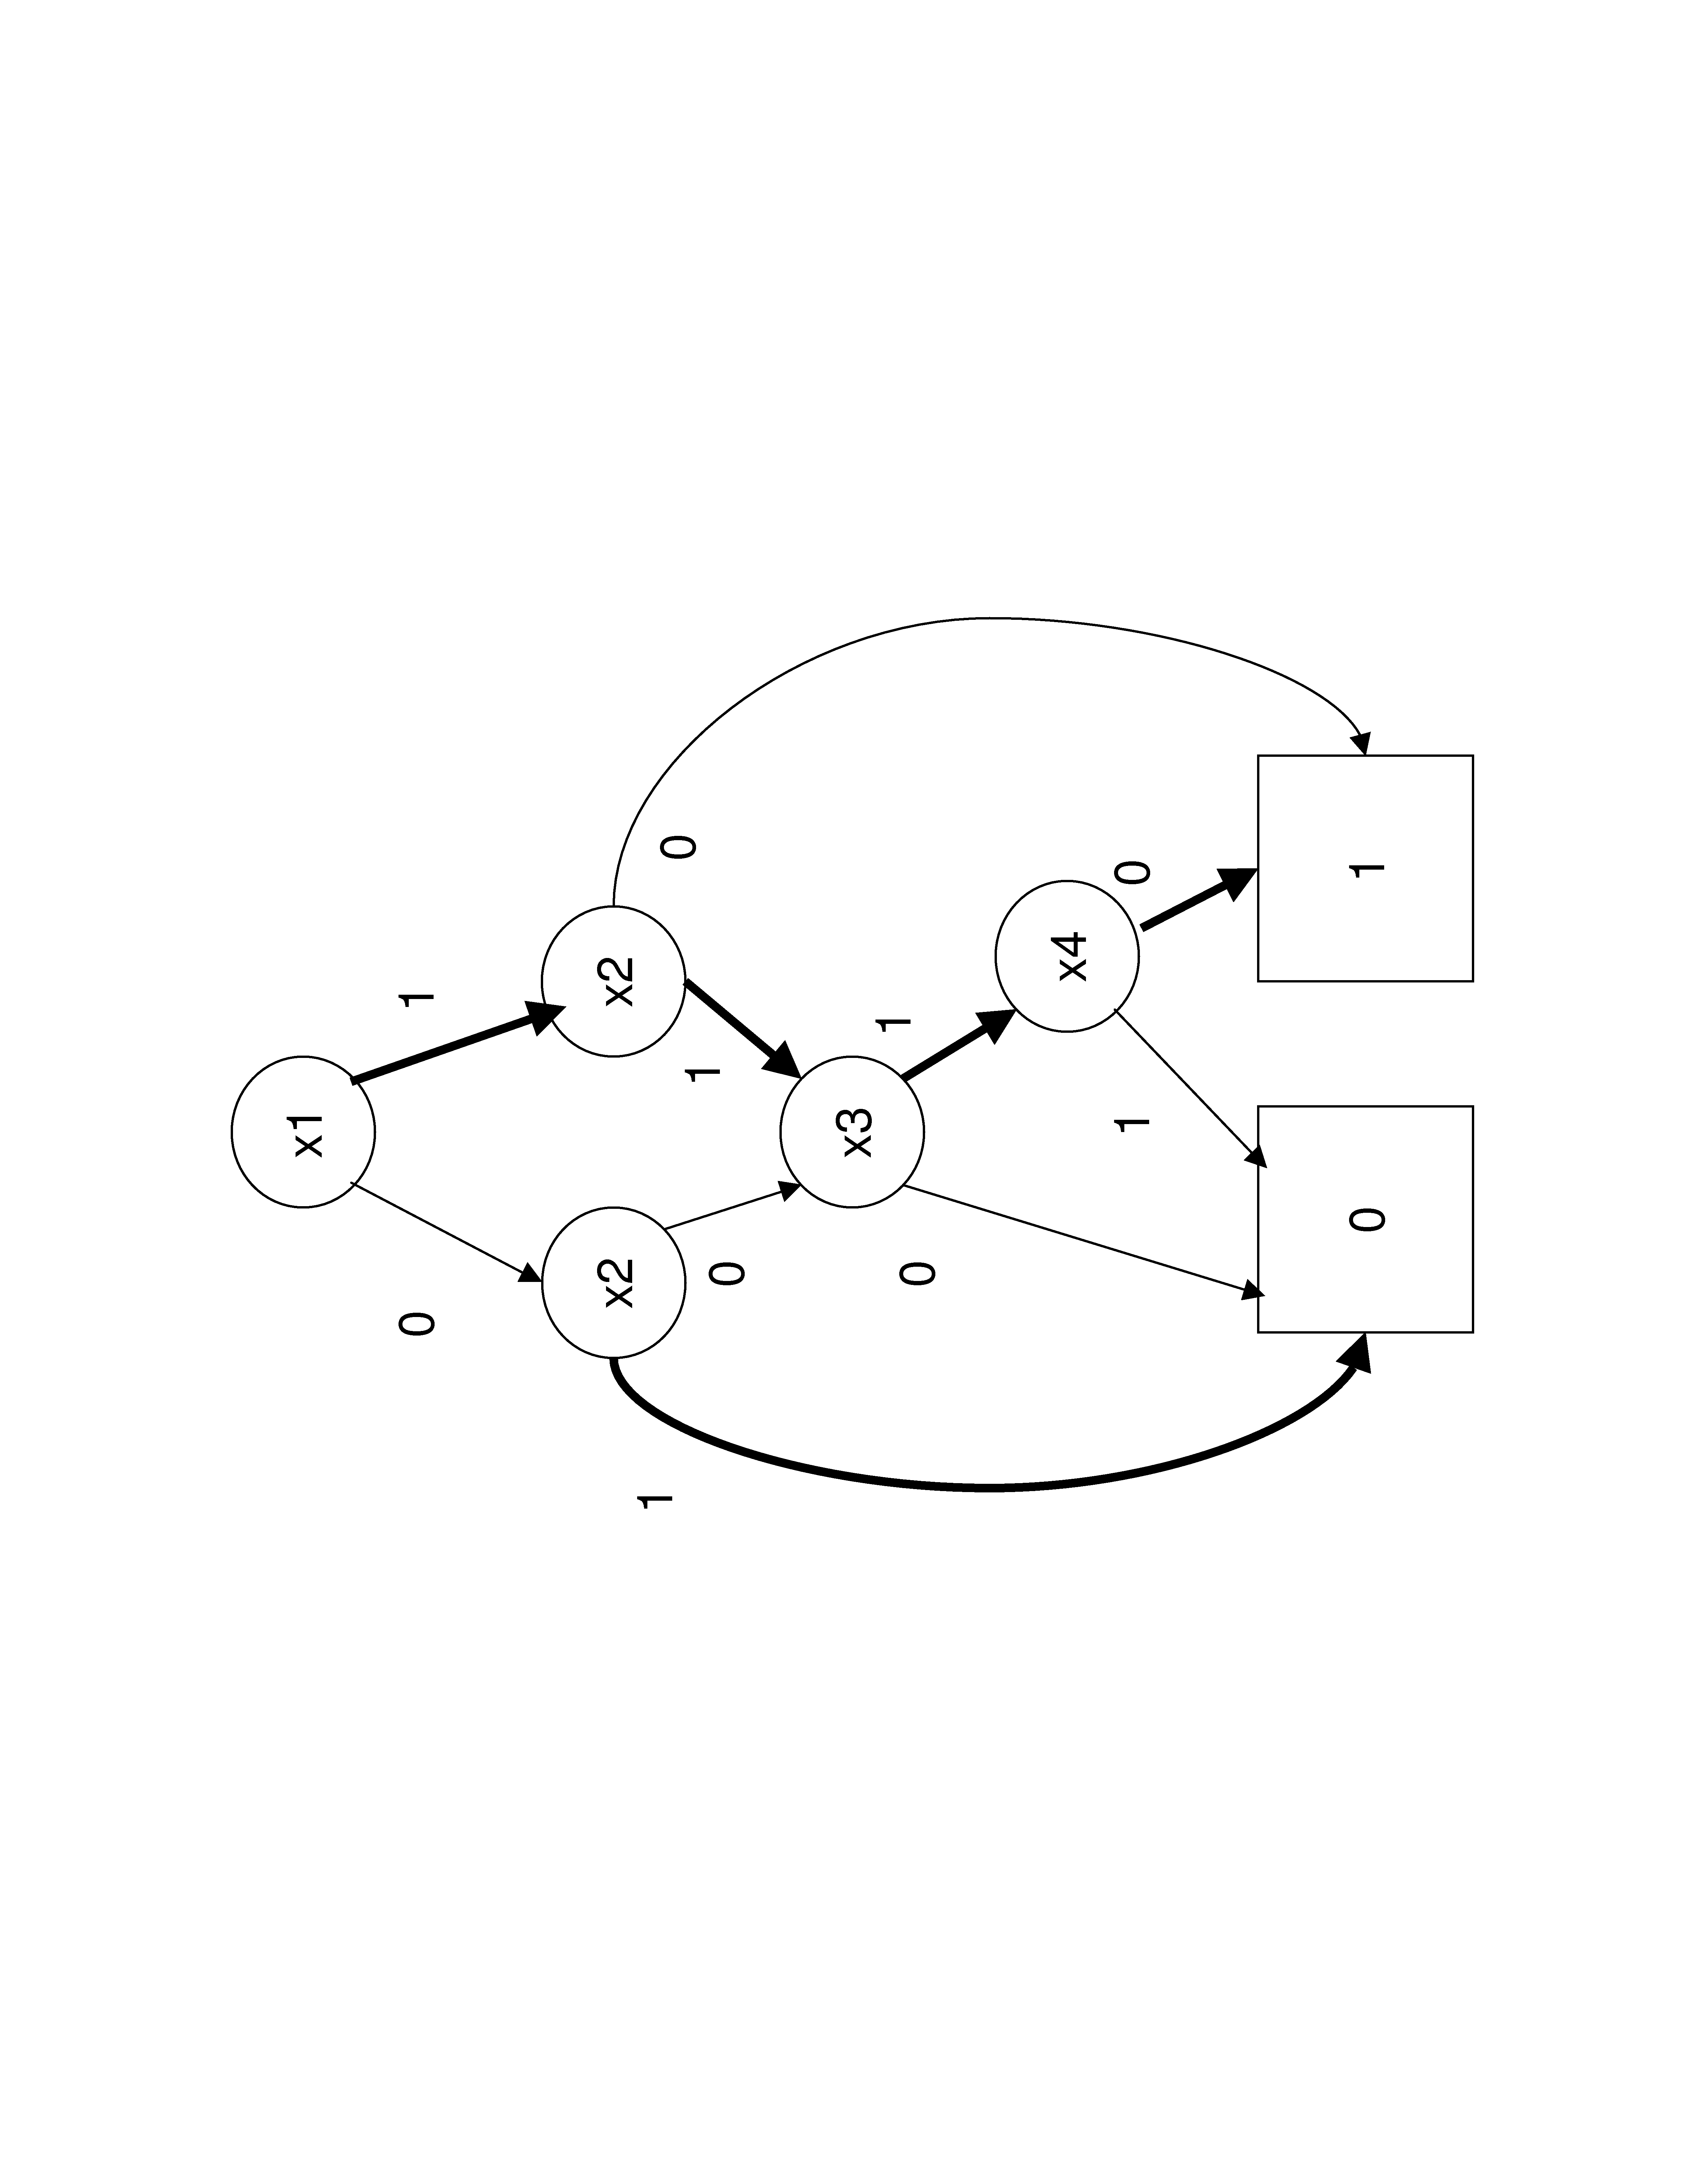
\includegraphics[scale=0.4,angle=270]{chapters/obdd1} 
\par\end{centering}

\caption{\label{fig:OBDD-example}OBDD for two-bit millionaires' problem}

\end{figure}


In \cite{kruger06}, we presented an SFE protocol that directly uses
an OBDD representation of the function $f$ to be jointly computed.
The advantage of using an OBDD representation over the Boolean gate-representation
is that OBDDs are more succinct for certain classes of functions than
the Boolean gate representation, including most linear functions.
For example, the OBDD representation is more efficient than the Boolean
gate representation for 8-bit AND, 8-bit addition, and the millionaires'
and billionaires' problems \cite{Yao86} OBDDs are not a universal
solution, however, for other functions, such as multiplication, the
OBDD can be far worse than the Boolean gate representation, due to
exponential node explosion \cite{Bryant:BDD}. For the classes of
functions in which the OBDD representation is efficient, our thesis
\cite{kruger06} shows that the protocol described next can perform
2 to 4 times better than the classical Yao protocol.

The protocol is loosely designed in a similar fashion as Yao's protocol
\cite{Yao86}. We present two variations of the protocol. An overview
of the 3 main steps of the protocols are shown in figure \ref{fig:OBDD-overview},
using the example millionaires' problem pictured above. In the first
step, Alice sends to Bob the encrypted OBDD. The next step is Bob
acquiring a subset of the encryption keys from Alice using $OT_{2}^{1}$.
In the final step, Bob uses the obtained keys to decrypt a single
path through the OBDD yielding the result of the computation. % A formal description follows. 


%
\begin{figure}
\begin{centering}
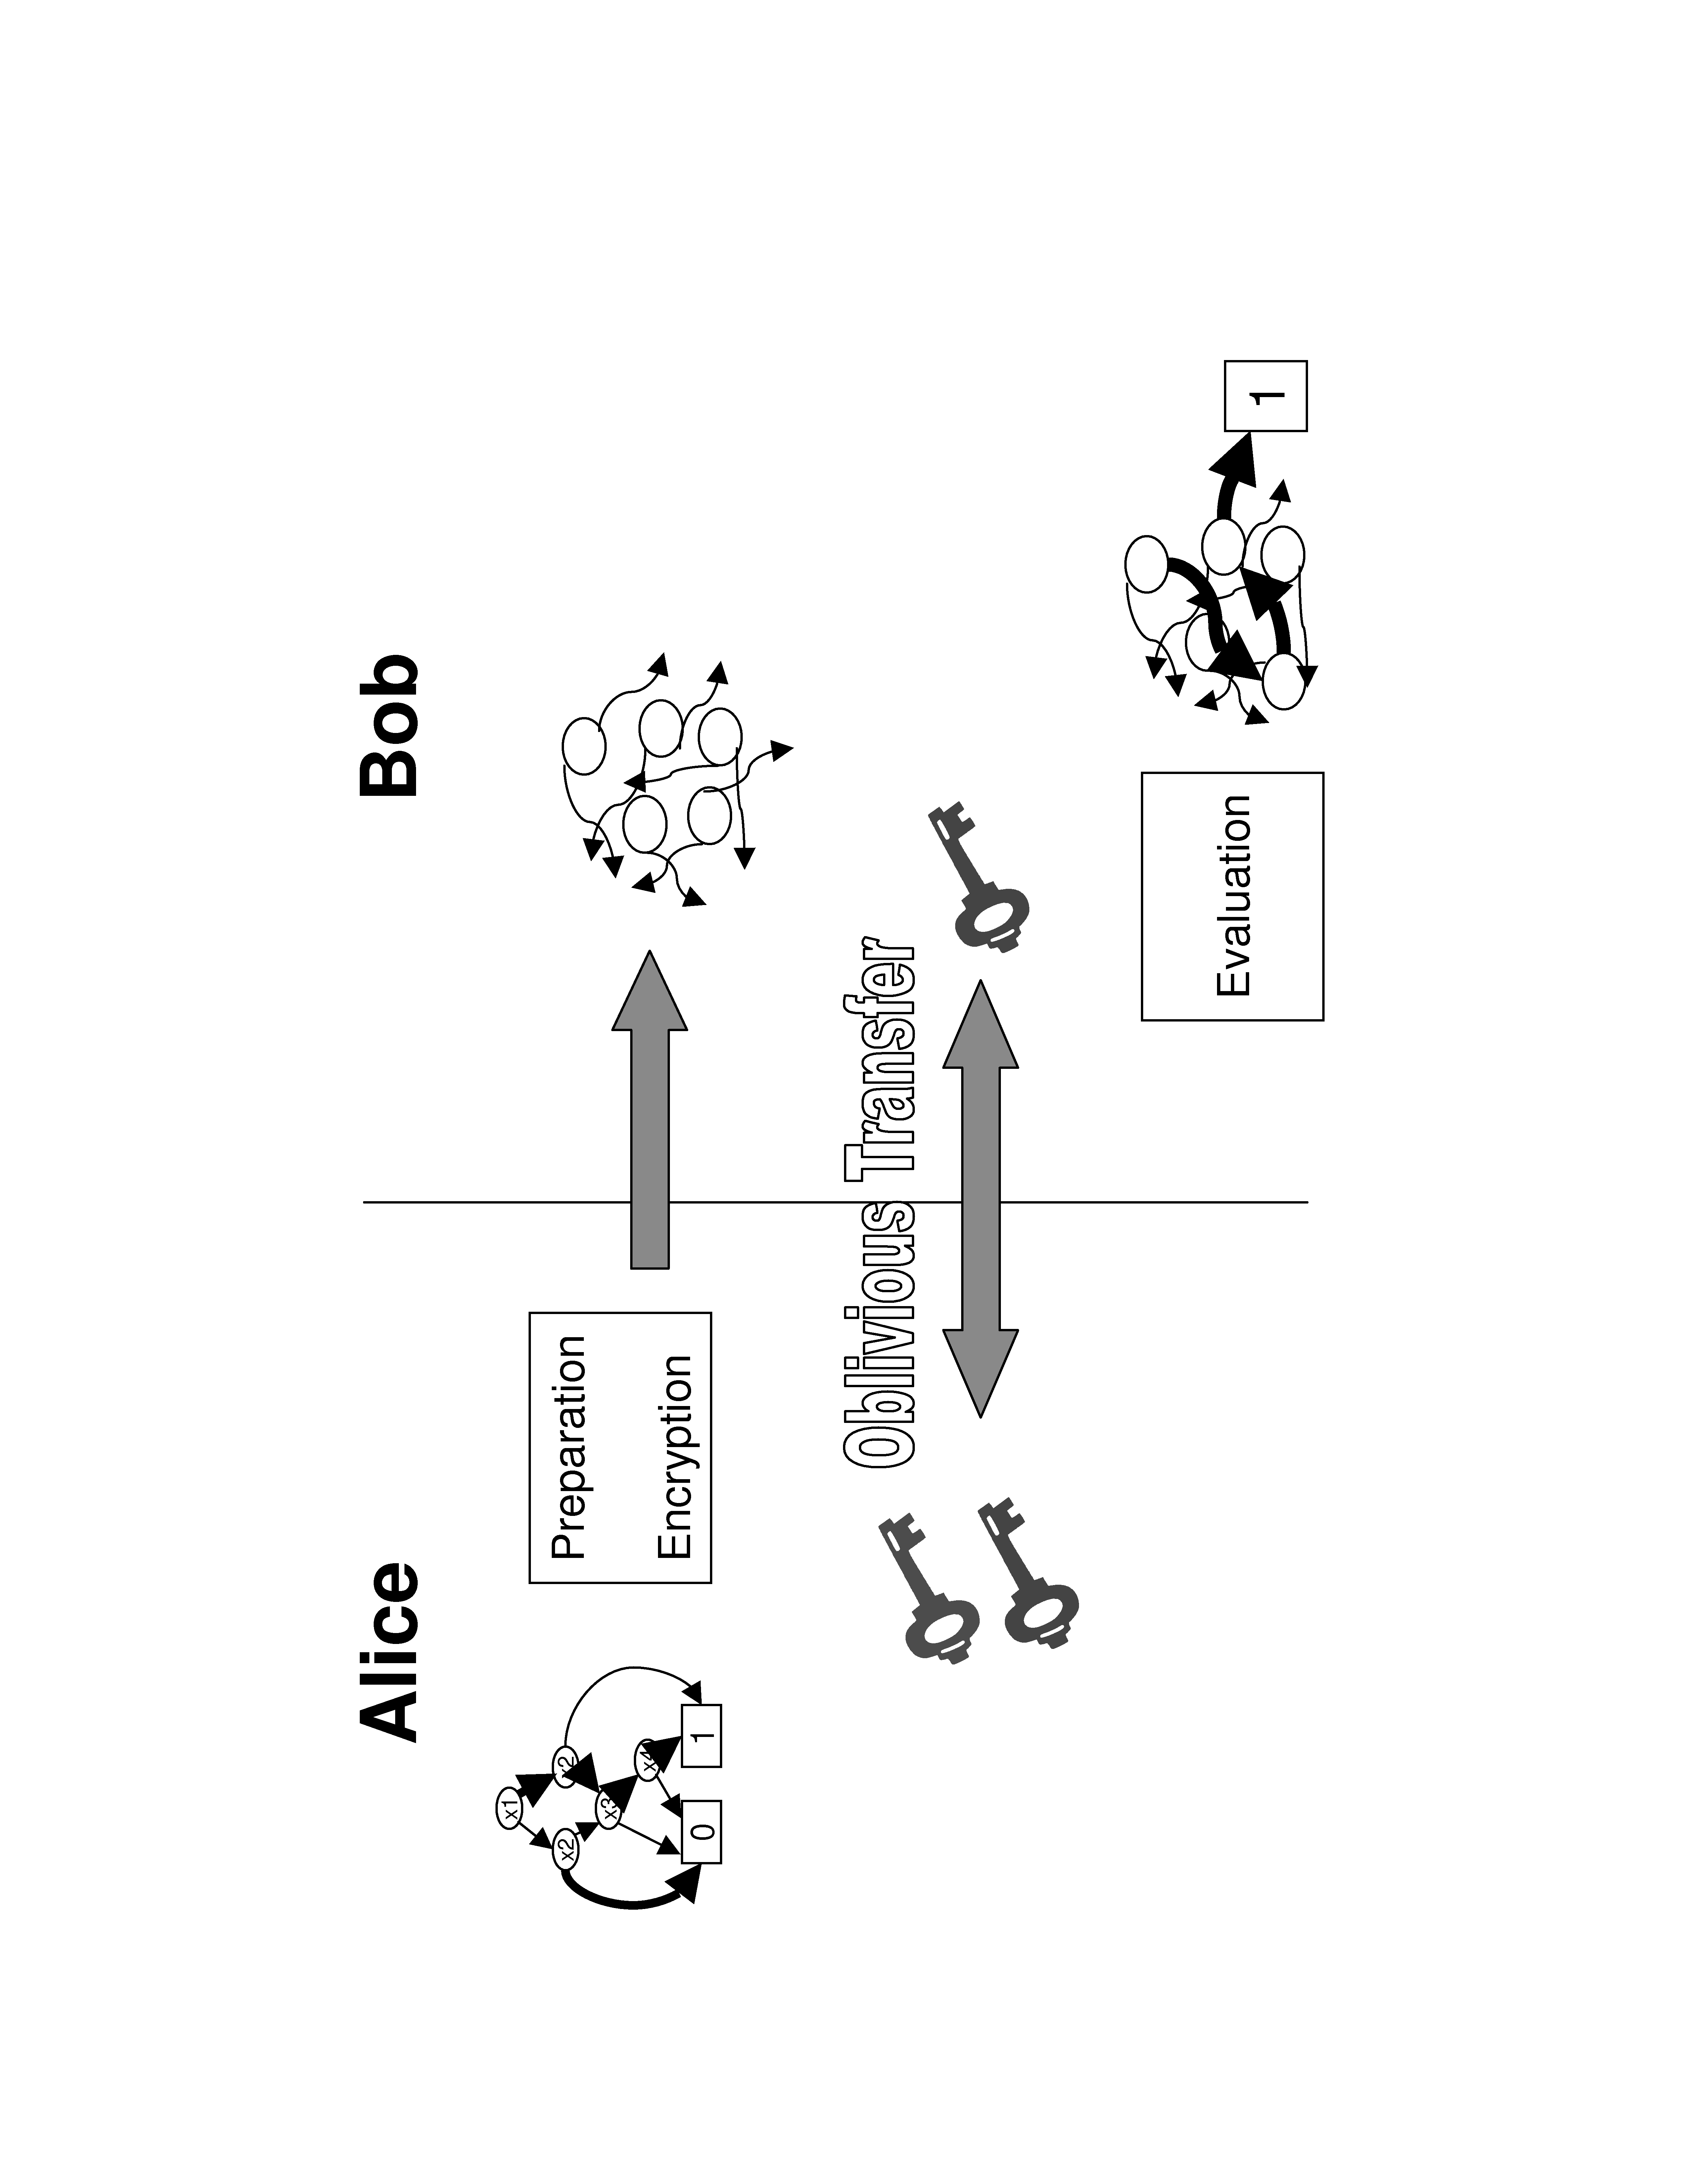
\includegraphics[scale=0.4,angle=270]{chapters/obdd_proto_overview} 
\par\end{centering}

\caption{\label{fig:OBDD-overview}OBDD secure evaluation protocol}

\end{figure}


%\begin{flushleft}
Assume that both parties' inputs include the $OBDD(f)$ for the Boolean
function $f(x_{1},x_{2},\cdots,x_{n})$ with the ordering $x_{1}<x_{2}<\cdots<x_{n}$.
Furthermore, Alice holds the inputs $(i_{1},\ldots,i_{k})$ corresponding
to the first $k$ variables $x_{1},\ldots,x_{k}$, and Bob has the
inputs $(i_{k+1},\ldots,i_{n})$.
\par\end{flushleft}
\begin{enumerate}
\item Alice performs the following steps: 

\begin{enumerate}
\item She traverses the $OBDD(f)$ using her input $(i_{1},\cdots,i_{k})$,
which results in a node $v_{init}$ at level $k$.
\item She uniformly and independently at random creates $(n-k)$ pairs of
secrets $(s_{1}^{0},s_{1}^{1}),\cdots,(s_{n-k}^{0},s_{n-k}^{1})$.
In addition, for each node $v$ in the $OBDD(f)$ whose level is between
$k$ and $n-1$, Alice also creates a secret $s_{v}$.
\item She assigns a uniformly random label to each node whose level is between
$k$ and $n$. We refer to the randomly assigned label of node $v$
using the notation $label(v)$.
\item Next, Alice augments $OBDD(f)$ with some number of dummy nodes (to
ensure that Bob always traverses $n-k$ nodes in his phase of the
protocol).
\item Alice garbles all nodes whose level is between $k$ and $n-1$ in
the following manner. Let $v$ be a node in $OBDD(f)$ such $k\leq{\it level}(v)\leq n-1$
and define ${\it level}(v)=\ell$. The encryption of node $v$, denoted
by $E^{(v)}$, is a label and a randomly ordered ciphertext pair \[
\left(label(v)\,\,,\,\, E_{s_{v}\oplus s_{\ell-k+1}^{0}}(label(low(v))\,\|\, s_{{\it low}(v)})\,\,\,,\,\,\, E_{s_{v}\oplus s_{\ell-k+1}^{1}}(label(high(v))\,\|\, s_{{\it high}(v)})\right)\,\,\,,\]
 where the labels are pre-pended to the secret with a separator symbol
and the order of the ciphertexts is determined by a fair coin flip.
Roughly speaking, the secrets corresponding to the $0$-successor
and $1$-successor of node $v$ are encrypted with the secret corresponding
to $v$ and its level.


Note that dummy nodes have the same structure as normal nodes, except
that the ciphertext pair contain encryptions of the same message since
dummy nodes have the same $0$ and $1$-successors. Provided the encryption
scheme is semantically secure, this poses no problem since the keys
are chosen uniformly at random.

Lastly, there are two terminal nodes of the form $(b,label(t_{b}))$
for $b=0$ or $1$. Recall that $OBDD(f)$ has two terminal nodes,
denoted as $0$ and $1$, that are at level $n$.

\item Once Alice is done encrypting, she sends to Bob the encryption of
all nodes whose level is between $k$ and $n$ and the secret $s_{v_{init}}$
corresponding to node $v_{init}$ at level $k$. We called this the
garbled OBDD.
\end{enumerate}
\item Bob performs the following steps: 

\begin{enumerate}
\item He engages in $n-k$ 1-out-of-2 oblivious transfers to obtain the
secrets corresponding to his input. For example, if his input $i_{j}$
is $0$, then he obtains the (level) secret $s_{j-k}^{0}$; otherwise,
he obtains the secret $s_{j-k}^{1}$.
\item Now Bob is ready to start his computation. Suppose $i_{k+1}=0$. With
$s_{1}^{0}$ and $s_{v_{init}}$, he decrypts both ciphertexts in
$E^{(v_{init})}$ and decides which gives the correct result by using
the verifiable range property of the encryption scheme. Bob now has
both $s_{{\it low}(v)}$ (the secret corresponding to the $0$-successor
of $v_{init}$) and $label(low(v))$ (which tells Bob which encrypted
node is used to evaluate his next input). Continuing this way, Bob
eventually obtains a label corresponding to one of the terminal nodes,
which determines the result of the OBDD on the shared inputs. Bob
sends this result to Alice. 
\end{enumerate}
\end{enumerate}




We then define an optimized variation which is identical to the protocol
just described, except that Alice first reduces the number of nodes
to be sent to Bob using an operation called \emph{restriction}, which
is a partial evaluation applied to OBDDs. Restriction is defined as
follows.

Given an $n$ variable Boolean function $f(x_{1},x_{2},\cdots,x_{n})$
and a Boolean value $b$, the restriction $f\mid_{x_{i}\leftarrow b}$
is a Boolean function of $n-1$ variables $x_{1},\cdots,x_{i-1},x_{i+1},\cdots,x_{n}$.
$f\mid_{x_{i}\leftarrow b}(x_{1},\cdots,x_{i-1},x_{i+1},\cdots,x_{n})$
is equal to $f(x_{1},\cdots,x_{i-1},b,x_{i+1},\cdots,x_{n})$. Essentially,
$f\mid_{x_{i}\leftarrow b}$ is the function obtained by substituting
the value $b$ for the variable $x_{i}$ in the function $f$. The
restriction operation can be performed over multiple variables by
restricting each variable independently, e.g., $f\mid_{x_{i}\leftarrow b,x_{j}\leftarrow b'}=(f\mid_{x_{i}\leftarrow b})\mid_{x_{j}\leftarrow b'}$.
The order in which the variables are restricted is unimportant.

\begin{flushleft}
For protocol 2, both parties' inputs include the $OBDD(f)$ for the
Boolean function $f(x_{1},x_{2},\cdots,x_{n})$ with the ordering
$x_{1}<x_{2}<\cdots<x_{n}$. Furthermore, Alice holds the inputs for
the variables in the set $X_{A}$ and Bob holds the inputs for the
variables in the set $X_{B}\;=\;\{x_{1},\cdots,x_{n}\}-X_{A}$. 
\par\end{flushleft}
\begin{enumerate}
\item Alice performs the following steps:

\begin{enumerate}
\item Alice computes the OBDD ${\cal O}_{A}$ as the restriction of her
inputs on the function $f\mid_{X_{A}}$. 
\item Alice encrypts the $O_{A}$ and sends it to Bob. This step is exactly
the same as in for Protocol 1. Alice also sends the secret corresponding
to the root of the OBDD ${\cal O}_{A}$. 
\end{enumerate}
\item The computation for Bob is exactly the same as that for Protocol 1. 
\end{enumerate}
The results of this work demonstrate that OBDDs showed improved performance
with secure evaluation of certain functions, as will be discussed
in chapter \ref{chapter:obdd}.

%\begin{comment}
\section{Problem Specific: Protocol Optimization of Evaluating Hash Functions
for Password Authentication}

In chapter \ref{chapter:pw}, based on our paper Secure Password Authentication
Using SFE \cite{Kruger10}, we use some properties of the problem
of authentication to transform the semi-honest protocol into an efficient
protocol that is secure in the malicious model. This work presents
a new solution to the {}``Secure Password and Key Authentication''
(SPAKA) problem, which is the design of protocols to mutually authenticate
a client to a server using 
\begin{enumerate}
\item The client's knowledge of the password X, and 
\item The servers's knowledge of a one-way hash function h(X). 
\end{enumerate}
The protocol must not leak any additional information or allow access
if one of the parties is an inposter and does not know their expected
credential. Our solution provides a property, unique among SPAKA protocols,
that it can work with arbitrary and legacy hash functions used in
commodity operating systems today. This protocol takes advantage of
specific properties of the authentication problem and takes {}``shortcuts''
to achieve efficiency. Although these shortcuts would not be secure
in a general SFE setting, we prove that these shortcuts are in fact
secure in the context of the authentication protocol presented. This
allows us to design a protocol in which a malicious adversary is thwarted
with probability $1-2^{-l}$ where $l$ is a security parameter representing
the number of semi-honest circuits. We show that on modern multicore
processors, the authentication can be performed in a matter of seconds,
which we believe is practical for interactive use between servers
and authenticating users.
%\end{comment}

\section{Class of Algorithm Specific: Protocol Optimization of Dynamic Programming}

In this work, presented in detail in chapter \ref{chapter:genomics},
we considered a design \emph{methodology} for creating secure protocols
based on typical dynamic programming algorithms. Unlike the OBDD protocol
discussed in the previous section, this is not an automatic tool for
generating secure protocols, but rather a set of concepts that are
applicable to designing secure protocols for evaluating dynamic programming
algorithms. We illustrate these ideas with several example protocols
for computing the edit distance problem, which is the minimum number
of character insertions, deletions, and substitutions needed to change
string $x$ to string $y$.

Let ${\cal P}(x,y)$ be a problem with two inputs $x$ and $y$. Typically,
a dynamic-programming algorithm ${\cal A}_{{\cal P}}$ for problem
${\cal P}$ has the following components: 
\begin{itemize}
\item A set $S$ of sub-problems and a dependency relation $R\subseteq S\times S$
between the sub-problems. Intuitively, $(s,s')\in R$ means that the
sub-problem $s'$ depends on the sub-problem $s$. If there is a dependency
between $s$ and $s'$, we write it as $s\rightarrow s'$. In the
case of the problem of computing edit-distance between two strings
$\alpha$ and $\beta$ of length $n$ and $m$, the set of sub-problems
is $[0,\cdots,n]\times[0,\cdots,m]$. For all sub-problems $(i,j)$
such that $i\not=0$ and $j\not=0$, we have the following dependencies:
$(i-1,j)\rightarrow(i,j)$, $(i,j-1)\rightarrow(i,j)$, and $(i-1,j-1)\rightarrow(i,j)$.
The \textit{base sub-problems} are $s\in S$ such that they have no
dependencies. For the edit-distance problem, the base sub-problems
are: \[
\begin{array}{l}
\{(i,0)\;\mid\;0\leq i\leq n\}\\
\{(0,j)\;\mid\;0\leq j\leq m\}\end{array}\]
 We also assume that there is a unique root sub-problem ${\it root}\in S$
such that there does not exist a sub-problem that depends on ${\it root}$.
For the edit-distance problem the unique root sub-problem is $(n,m)$. 
\item Each sub-problem $s$ is assigned a value ${\it val}(s)$. The goal
is to compute ${\it val}({\it root})$. The function ${\it val}$
from $S$ to $\Re$ assigns values to sub-problems, such that it satisfies
the following properties:

\begin{itemize}
\item For all the base sub-problems $s\in S$, ${\it val}(s)$ is defined. 
\item Let $s\in S$ be a non-base sub-problem. Define ${\it pred}(s)$ as
all the predecessors of $s$, i.e. the set ${\it pred}(s)$ is defined
as $\{s'\;\mid\; s'\rightarrow s\}$. Assume that ${\it pred}(s)$
is equal to $\{s_{1},\cdots,s_{k}\}$. There is a recursive function
$f$ defining ${\it val}(s)$ in terms of ${\it val}(s_{1}),{\it val}(s_{2}),\cdots,{\it val}(s_{k})$,
$s(x)$, and $s(y)$, where $s(x)$ and $s(y)$ are parts of the input
$x$ and $y$ that are relevant to the sub-problem $s$. In case of
the edit-distance problem ${\it val}((i,j))$ is equal to $D(i,j)$. 
\end{itemize}
\end{itemize}
We implemented three variations of the protocol in \cite{kruger07},
and showed that the techniques produce efficient ways to compute the
edit distance of two strings. For example, the protocol is able to
compute the edit distance of two strings of length $200$ (which has
$200^{2}=40000$ sub-computations), in under 10 minutes. Our most
efficient protocol computes elements of the dynamic programming matrix
in large blocks during each round of the computation. We experimentally
determined than a block size of $(20,20)$ yielded an optimum trade-off
between a decreased number of rounds, and larger block circuits. Using
a $(20,20)$ circuit allows $20^{2}=400$ elements of the matrix to
be evaluated during each round of the protocol, which allows the overall
$(200,200)$ problem to be evaluated in $100$ rounds. In comparison,
using the generic techniques to compile the edit distance algorithms
into a secure circuit produced circuits which were to too large for
evaluation beyond problems of size $(25,25)$.


\section{Algorithm Specific: Protocol Optimization of K-Means Clustering}

The $k$-means algorithm is a common clustering technique in data
mining. Suppose that we are given $n$ samples $x_{1},\cdots,x_{n}$,
where each sample is a $m$-dimensional vector of real numbers. The
problem is to assign the samples to $c$ clusters in such a manner
that similar points are grouped together. Similarity is defined using
a distance metric. The standard clustering algorithm maintains $c$
means $\mu_{1},\cdots,\mu_{c}$. Initially, assume that the means
are assigned arbitrary values. A sample $x_{i}$ is deemed to be in
the cluster $j$ if it is closest to the mean $\mu_{j}$, where mean
of a cluster $\{x'_{1},\cdots,x'_{r}\}$ is $\frac{x'_{1}+\cdots,x'_{r}}{r}$.
In a Euclidean space, the distance between two $m$-dimensional vectors
$x$ and $y$ is $\sum_{j=1}^{m}(x[j]-y[j])^{2}$, where $x[j]$ is
the $j$-th element of the vector $x$. Other distance metrics~\cite[Chapter 10]{pattern-classification},
such as scatter metrics, can be used instead of the distance metric
mentioned above. Each iteration of the $k$-means algorithms recomputes
the means and reclassifies the samples. The algorithm terminates when
it detects no change in the means. See \ref{fig:clusters} for an
illustration.

%
\begin{figure}
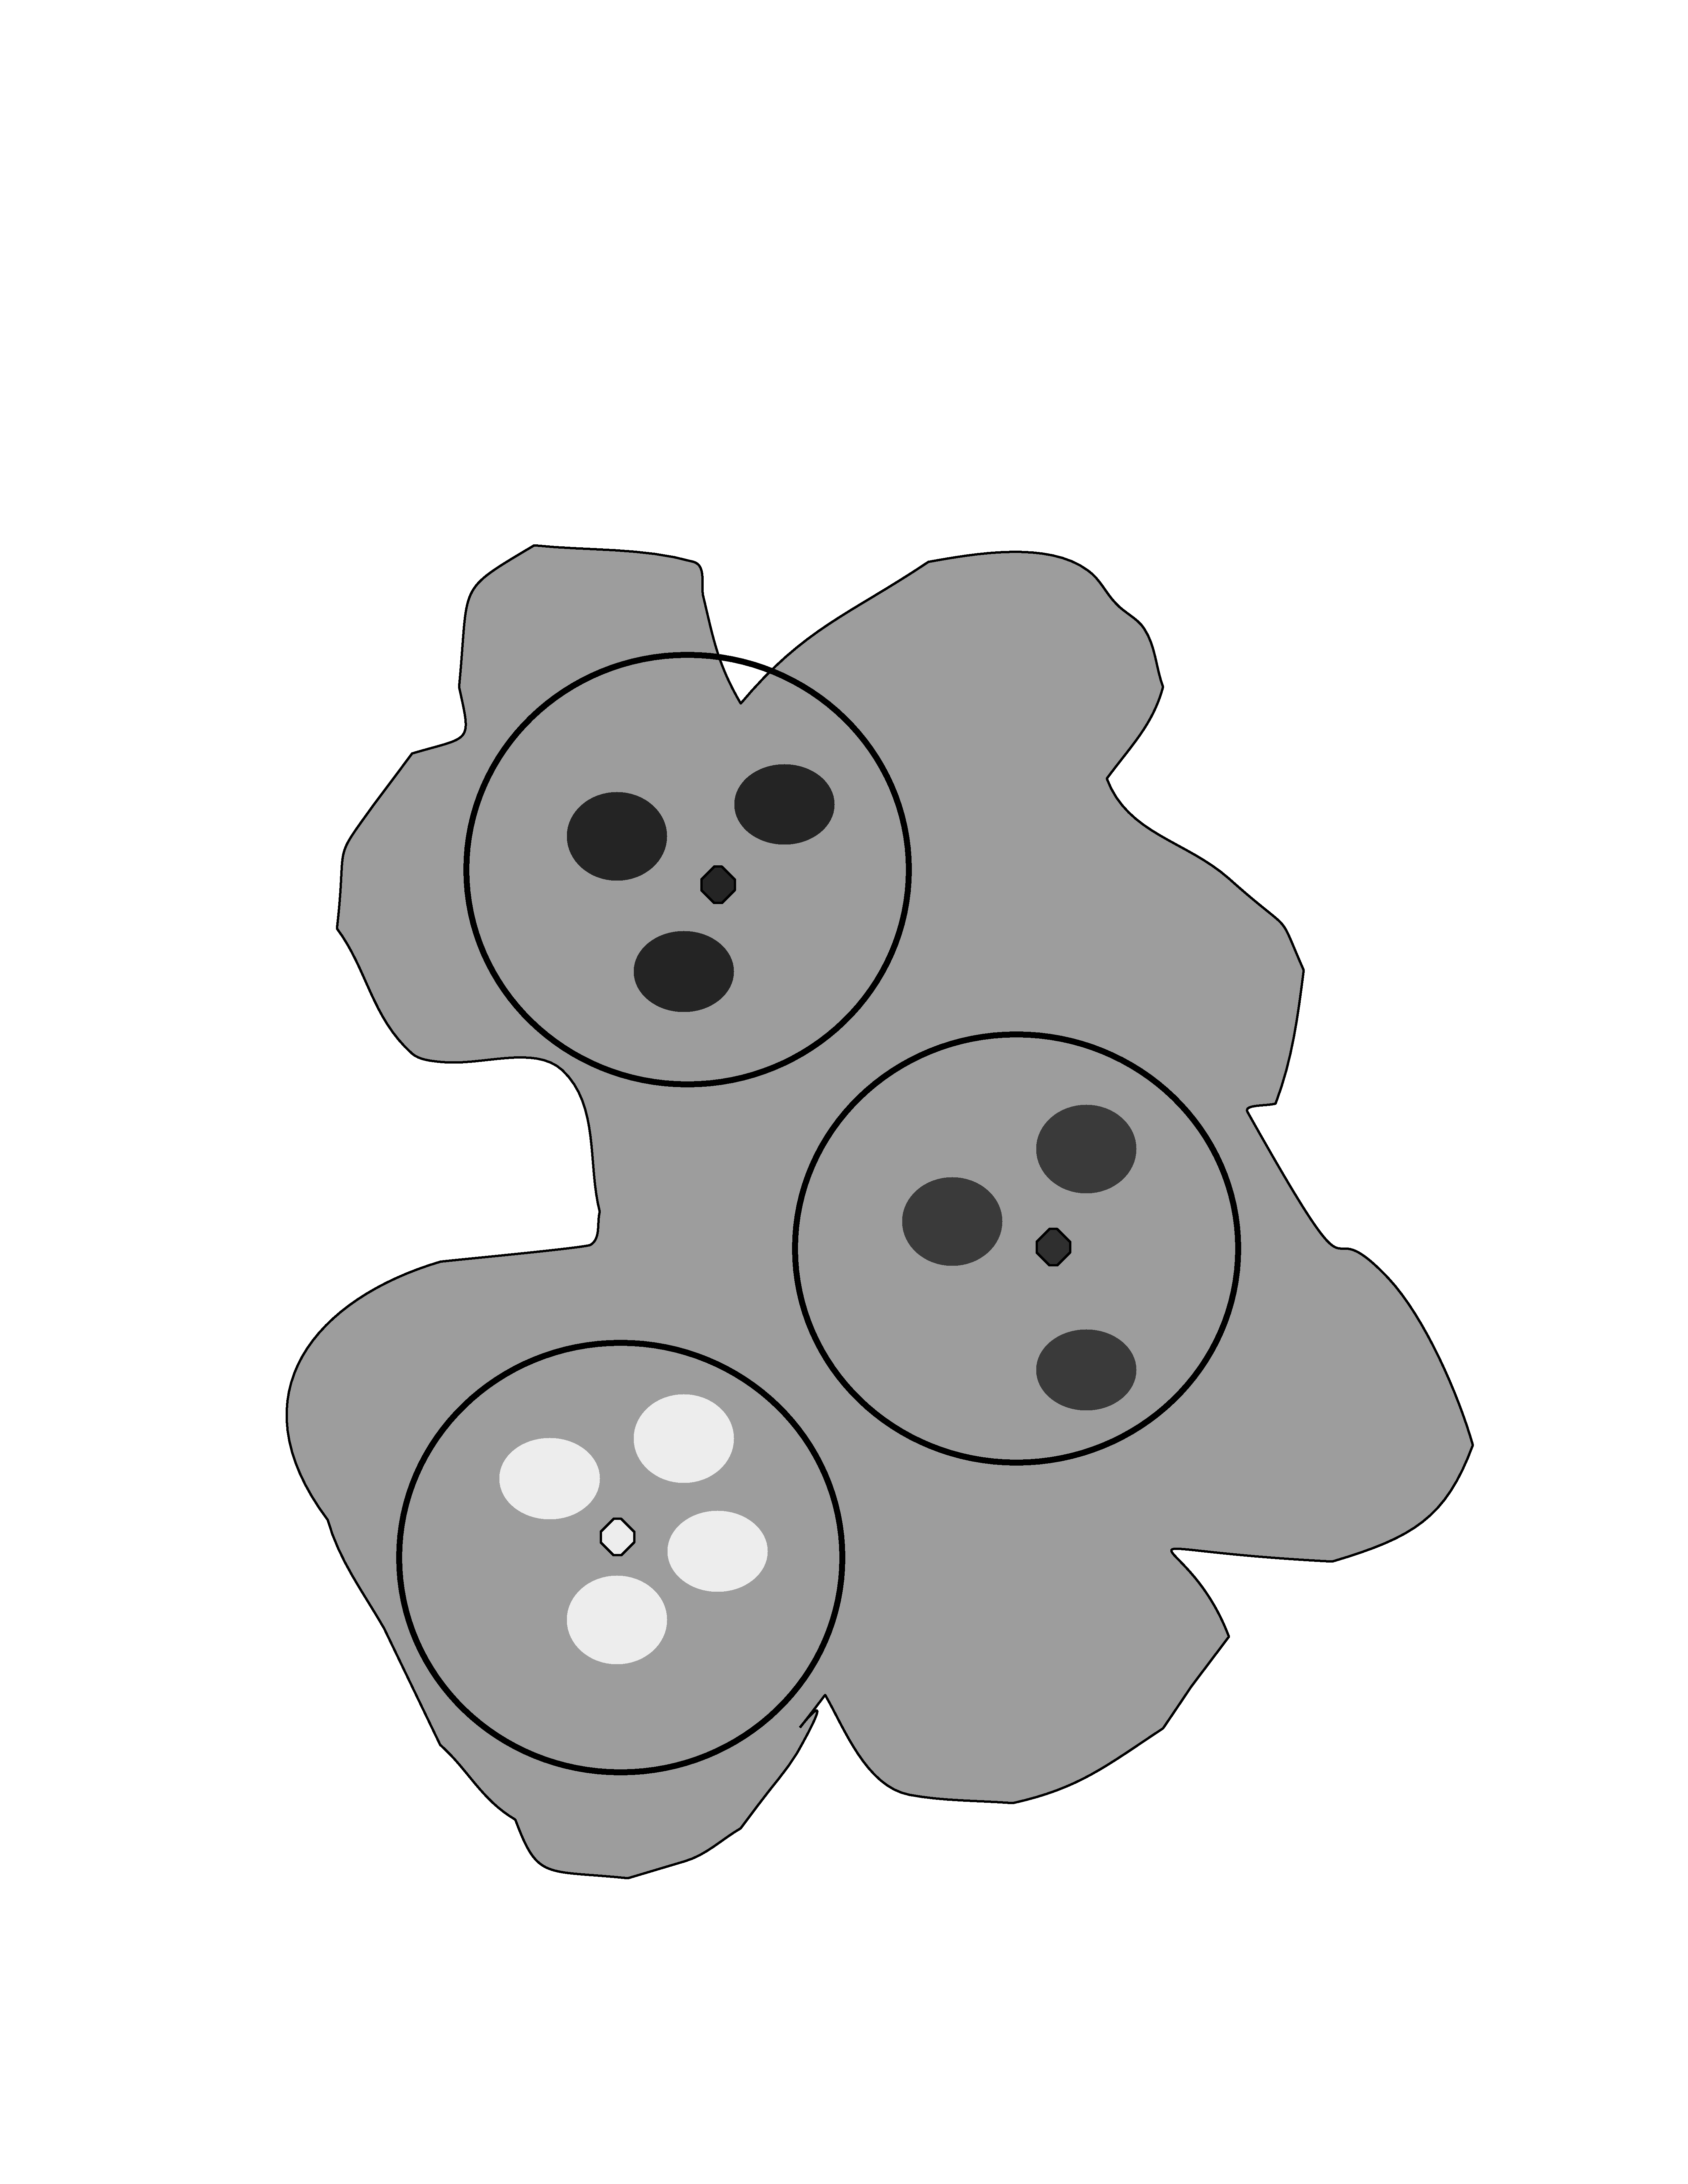
\includegraphics[scale=0.3,angle=270]{chapters/clusters}

\caption{\label{fig:clusters}Thirteen data points after clustering. The small
dots are cluster means.}

\end{figure}


We implement protocols to securely evaluate this algorithm in chapter
\ref{chapter:kmeans} based on our paper \cite{kruger05}, and showed
that a protocol based on homomorphic encryption was able to classify
partitioned data sets with tens of thousands of data points in under
two minutes, which is about 15 times slower than the protocol implemented
without privacy protection, and over 100 times faster than the same
protocol built with Yao circuits.


\section{Other Optimizations}

\label{sub:Other-Optimizations}

In the usual formulation of secure function evaluation, there are
designated outputs for each party, and it is required that no extra
information is learned by any party. This definition could be expanded
to assign non-output values the labels {}``sensitive'' and {}``non-sensitive'',
where the protocol is considered secure if no sensitive information
is leaked. %Since the overhead of privacy protection is substantial,
%I propose to research the of design secure protocols that use this
%relaxation of the problem definition to improve efficiency. 


In section \ref{sub:Primitives}, I presented many basic cryptographic
primitives that are used in SFE. Improving the state of the art of
any one of those primitives would automatically benefit all SFE protocols
that make use of that primitive. Based on my experience with real
implementations of SFE protocols, the oblivious transfer steps tend
to be very expensive in terms of space and communication. Common oblivious
transfer protocols are based on discrete logarithms, but other trapdoor
functions may be used as well. %One thing I propose to try is implementing
%Naor-Pinkas \cite{Noar-Pinkas:2001} using more compact representations,
%for example, with elliptic curve groups. I have recently developed
A new $OT_{2}^{1}$ protocol is presented in chapter \ref{sec:OT-SquareRoots}.
and its security and performance are compared with the Naor-Pinkas
protocol. %In particular, I conjecture that this protocol
%may require less communication overhead than other OT protocols.


%
\begin{comment}

\chapter{An Efficient Protocol Design Framework}

\label{sub:An-Efficient-Framework}

Even with all these optimizations, protocols still must be hand-coded.
Each protocol I have implemented has required brand new code to be
written, with only some common cryptographic primitives being shared
between implementations. In this case, I define the term protocol
to mean a structured sequence of communications between parties which
enables the computation to performed. Fairplay \cite{Fairplay} suggested
the idea of having a common framework for protocol design, but because
Fairplay is a straightforward implementation of Yao's garbled circuit
method \cite{Yao86}, it suffers from poor performance. Fairplay's
contribution is to create a compiler for expressing algorithms functionally,
and compiling them into a circuit representation suitable for secure
evaluation. In this sense, it functions as a simple CAD design tool.

I propose to take this concept much further, and create an \emph{optimizing}
protocol compiler, aggregating the techniques discussed here, and
creating a tool to greatly simplify the creation of efficient secure
protocols for SFE. The compiler will include the following components: 
\begin{itemize}
\item Convenient programming language for expressing secure computations

\begin{itemize}
\item Language will include support as language primitives for common SFE
and cryptographic techniques, such as homomorphic encryption 
\item Language will support metadata for designating inputs and outputs
from specific parties, and for classifying the required privacy of
intermediate computations 
\end{itemize}
\item Compiler which translates this language into an abstract securely
evaluable {}``machine code'', which consists of securely evaluable
representations of the program. 
\item An automated optimizer. The optimizer will automatically try different
representations of the functions, including OBDDs, Boolean circuits,
and other ideas from my research, and search for the most efficient
representation as possible. 
\item Manual optimization tools, making it convenient to apply and design
techniques that I have researched. This includes a toolkit of cryptographic
protocols, such as oblivious transfer, which can be used in a black
box way. 
\item An embeddable protocol evaluator library, which will allow ordinary
application to make straightforward use of secure function evaluation. 
\end{itemize}
The security of protocols produced by the compiler is based on the
security of each individual component of the protocol. For example,
when choosing optimal circuit representations, the compiler will choose
among several possible representations, each of which has a corresponding
secure evaluation protocol. In cases where a computation is broken
into multiple sub-protocols, I will prove that composition of these
sub-protocols maintains the overall security of the protocol.

\bibliographystyle{plain} \bibliographystyle{plain}
\bibliography{somesh}

\end{comment}
{} 



\chapter{Oblivious Transfer with Modular Square Roots}\label{sec:OT-SquareRoots}
\label{chapter:otquad}

A new $OT_{2}^{1}$ protocol is presented, using the square root function
in modular multiplicative groups as a trapdoor function. Here, I present
a informal sketch of correctness, security, and efficiency. I propose
to complete the proofs and perform a thorough experimental evaluation
of its performance with respect to other oblivious transfer protocols.


\section{Protocol}
\begin{enumerate}
\item The sender chooses large random prime numbers $p$ and $q$ such that
$p\equiv q\equiv3\;(\mbox{mod }4)$ and calculates $n=pq$. $n$ is
sent to the chooser. This is a one time setup step that need not be
repeated for subsequent uses of the protocol.
\item The chooser uniformly chooses a random value $x\in S\subset Z_{n}^{*}$
where $S=\{z\in Z_{n}^{*}:$~$z\le\frac{n-1}{2}\mbox{ and }$ $\left(\frac{z}{n}\right)=-1$
if $s=1$ otherwise $\left(\frac{z}{n}\right)=+1\}$. The chooser
computes $y\equiv x^{2}(\mbox{mod }n)$ and sends $y$ to the sender.
$\left(\frac{x}{n}\right)$ denotes the Jacobi symbol of $x$ and
$n$.
\item The sender calculates the square roots $a^{2}\equiv b^{2}\equiv y\;(mod\, n)$
such that $\left(\frac{a}{n}\right)=-1$ and $\left(\frac{b}{n}\right)=+1$
and $a,b\le\frac{n-1}{2}$
\item The sender encrypts $E_{a}(m_{1})$ and $E_{b}(m_{2})$ and sends
them to the chooser.
\item The chooser computes $D_{x}(E_{x}(m_{s}))$ to decrypt the output.
\end{enumerate}

\section{Correctness}

$\left(\frac{x}{n}\right)=-1$ for half the elements $x\in Z_{n}^{*}$
. $\left(\frac{x}{n}\right)=+1$ for the other half. Thus the chooser
can always successfully perform step 2.

If $a^{2}\equiv b^{2}\;(mod\; n)$ and $a\neq\pm b\;(mod\; n)$ then
$\left(\frac{a}{n}\right)=-\left(\frac{b}{n}\right)$.%
\footnote{This follows when $p\equiv q\equiv3\ (\mbox{mod 4})$ from the properties
of the Jacobi symbol and the Chinese Remainder Theorem.%
} Furthermore, the set $\{a,b,n-a,n-b\}$is the complete set of square
roots of $y$. If $a>\frac{n-1}{2}$ then $a$ and $n-a$ can be swapped,
and similarly for $b$. Thus, the sender can always successfully complete
step 3. It is guaranteed that either $a=x$ or $b=x$ so the chooser
will successfully learn $m_{s}$ as intended.


\section{Security}

Finding all square roots of any quadratic residue in $Z_{n}^{*}$
can be reduced to factoring $n$. This is because given two principal
square roots $a^{2}\equiv b^{2}$, $a\neq-b$, then $(a-b)(a+b)\equiv0$
so $(a-b)(a+b)=kpq$ Under the standard complexity assumption that
factoring $n$ is infeasable, then the chooser can not efficiently
learn the other square root of $x^{2}$, which is the encryption key
of $E(m_{3-s})$ and the sender's privacy is preserved. 

The chooser's privacy is preserved because the sender does not know
whether the chooser calculated $y=a^{2}$ or $y=b^{2}$. From the
sender's perspective, the chooser has chosen $x$ from a uniform random
distribution $1\le x\le\frac{n-1}{2}$, so there is no information
that can be gained. The chooser therefore enjoys unconditional security
even without making assumptions about the senders computation power.


\section{Efficiency}

In the setup phase, the sender needs to calculate $n=pq$ once and
send the value of $n$ to the chooser. This requires one multiplication
and transmission of $k=\log n$ bits. The same value of $n$ can be
reused for subsequent or batched OTs without loss of security. $k$
must be large enough to prevent efficient factoring of $n$.

From then on, each OT requires the following: 
\begin{enumerate}
\item Computation of Jacobi symbols $\left(\frac{x}{n}\right)$ by the chooser.
If the chooser uses random trials to find an appropriate $x$, then
the expected number of trials is $2$. Computing Jacobi symbols can
be performed in $O(k\log x)\le O(k^{2})$ steps \cite{1996-bach-book}. 
\item There is a potential optimization of step 1. The chooser can pre-compute
a single number $\alpha$ where $\left(\frac{\alpha}{n}\right)=-1$.
From then on, the chooser can choose any random $\beta$ and have
$\left(\frac{\beta^{2}}{n}\right)=+1$ and $\left(\frac{\alpha\beta^{2}}{n}\right)=-1$.
This optimization as presented is insecure, because it breaks statistical
indistinguishability for the chooser~%
\footnote{The optimization will never produce a non-QR with $+1$ Jacobi symbol%
}. However, I speculate that there may exist a variation which avoids
this flaw and thereby reduces the chooser's overall complexity to
$O(k)$.
\item Transmission of a single $k$ bit number from chooser to sender
\item Computation by the sender of square roots of $y$. This can be performed
using a randomized algorithm in expected time $O(k\ \log\, p^{2})\le O(k^{3})$
steps for $p>q$ \cite{1996-bach-book}. 
\item Encryption and transmission by the sender of the two messages. If
the sender does not need to hide the length of the unreceived message,
then this requires no more bandwidth than the actual size of the messages,
which is $O(\log m)$
\item Decryption by the receiver of one of the messages, which is $O(\log m)$.
\end{enumerate}
If the sender and chooser wish to execute the protocol multiple times,
the chooser can simply send a vector $[y_{1},\cdots,y_{j}]$ and the
chooser will respond with a vector of tuples $[(E_{a_{1}}(m_{1_{1}}),(E_{b_{1}}(m_{1_{2}}))\cdots(E_{a_{j}}(m_{j_{1}}),(E_{b_{j}}(m_{j{}_{2}}))]$
where $j$ is the number of messages to be sent obliviously. Each
$x_{i}$ is an independent random variable so the security is equivalent
to the single message case. Thus, unlimited bits can be transferred
with a single network round-trip.


\section{Comparison with Naor-Pinkas\label{sub:Comparison-with-Naor-Pinkas}}

In the Naor-Pinkas protocol \cite{Noar-Pinkas:2001}, the computational
requirement for each party is $O((\log n)(\log\log n))$ for both
parties, where $n$ is the size of a group sufficiently large such
that calculating discrete logarithms is infeasible. The communication
consists of a message of size $\log n$ from sender to chooser, a
message of size $\log n$ from chooser to sender, and two messages
of size $\log m+\log n$ from sender to chooser, where $\log m$ is
the size of the chooser's outputs. The protocol presented here cuts
the final messages to $\log m$, which effectively reduces the bandwidth
with a tradeoff in computation time. My experimentation with running
SFE algorithms using fast modern CPUs indicates that this tradeoff
may be worthwhile. I plan to make empirical measurements with implementations
of the to comparitively measure the actual performance.


\section{Extensions}

It may be possible to extend the construction to cover the more general
$OT_{k}^{1}$. I have not investigated this yet, but one idea is to
let $n=\prod_{i=1}^{k}p_{i}$ where each $p_{i}$ is a large prime
number. In $Z_{n}^{*}$, each quadratic residue will have $2^{k}$
square roots consisting of $2^{k-1}$ pairs $(x,n-x)$

%
\begin{comment}
\bibliographystyle{plain}
\bibliography{crypto,privacy,somesh}

\end{comment}
{}




%
\begin{comment}
\input{newidea.tex}
\end{comment}
{}

%% LyX 1.6.1 created this file.  For more info, see http://www.lyx.org/.
%% Do not edit unless you really know what you are doing.
\documentclass[english]{article}
\usepackage[T1]{fontenc}
\usepackage[latin9]{inputenc}
\usepackage{geometry}
\geometry{verbose,letterpaper,tmargin=1.25in,bmargin=1.25in,lmargin=1.25in,rmargin=1.25in}
\setlength{\parskip}{\medskipamount}
\setlength{\parindent}{0pt}
\usepackage{verbatim}
\usepackage{graphicx}

%%%%%%%%%%%%%%%%%%%%%%%%%%%%%% Textclass specific LaTeX commands.
\newenvironment{lyxcode}
{\par\begin{list}{}{
\setlength{\rightmargin}{\leftmargin}
\setlength{\listparindent}{0pt}% needed for AMS classes
\raggedright
\setlength{\itemsep}{0pt}
\setlength{\parsep}{0pt}
\normalfont\ttfamily}%
 \item[]}
{\end{list}}

%%%%%%%%%%%%%%%%%%%%%%%%%%%%%% User specified LaTeX commands.

\linespread{1.1}

\usepackage{babel}

\begin{document}

\section{Strengthening SSH Password Authentication}

\subsection{Overview}

SSH is the predominant application for interacting with remote
systems. It was designed as an alternative to telnet with the purpose
of addressing the growing need for confidentiality, authentication,
and integrity. It has since evolved into a layered protocol, that can
serve as a secure transport layer over which other protocols can run
for enhanced security. This has increased its popularity to the point
where many of its users simply assume that it provides all of the
security they need.

However, SSH is currently vulnerable to a man in the middle attack
that allows the perpetrator to impersonate either the client or
server, or compromise the client's password. Many assume that this is
not the case because of SSH's host key authentication mechanism, but
there are a number of ways that an attacker can thwart the protection
it provides. For example, any SSH user is certainly familiar with the
following type of message:
\begin{verbatim}
   The authenticity of host 'server (1.2.3.4)' can't be established.
   RSA key fingerprint is 3f:76:22:43:c2:03:b9:71:b0:31:ce:87:37:45:cb:02. 
   Are you sure you want to continue connecting (yes/no)?
\end{verbatim}
In many usage scenarios, it is unreasonable to expect that the client
has verifiable access to the host's RSA key fingerprint before
attempting connection. In these cases, the user is left with a tough
decision; either accept the key's authenticity with no real evidence,
or forgo access to the host's services. This gives an attacker
leverage, and a likely chance at success.

Recent research in related areas has seen the development of a class
of authentication protocols dubbed SPAKA (\textit{Secure Password and
  Key Authentication})~\cite{bellovin92}. SPAKA protocols are designed
to guarantee confidentiality of secrets even against active
adversaries. A recent SPAKA protocol for resisting password compromise
in the event of host compromise~\cite{brainard03} suggests that secure
function evaluation can be applied generally to the problem of
developing SPAKA protocols.

With this in mind as a starting point, we apply SFE to the problem of
developing a SPAKA protocol suitable for authenticating SSH
connections, thus thwarting the MITM attack described earlier. Using
the client's password on the host as a shared secret, we observe that
the authenticity of the host (and the client) can be verified by
securely computing a variant of the millionaire problem. Specifically,
we provide the two parties with a way of determining whether the other
has access to the shared secret, without potentially revealing the
secret to a potential adversary.

In the following sections, we outline the relevant aspects of the SSH
protocol (Section 1.2), detail the nature of the man in the middle
attack on SSH's authentication mechanism (Section 1.3), present our
proposed solution in further detail (Section 1.4), describe our
implementation (Section 2), and talk about related work (Section 3).


\subsection{SSH Protocol Overview}

The SSH protocol is defined in terms of layers, much like the OSI
networking stack. Each layer is defined in terms of messages from the
underlying layer. The lowest level is a packet-based transport
protocol that is layered on top of TCP. All SSH messages of the higher
layers are sent as packets. This packet protocol is known as the SSH
transport layer protocol and is defined in \cite{rfc4253}.  Figure
\ref{fig:ssh-overview} shows the hierarchy of the ssh protocol layers
discussed here. The SSH transport layer also handles the server key
authentication, encryption, and integrity of a session.

%
\begin{figure}[t]
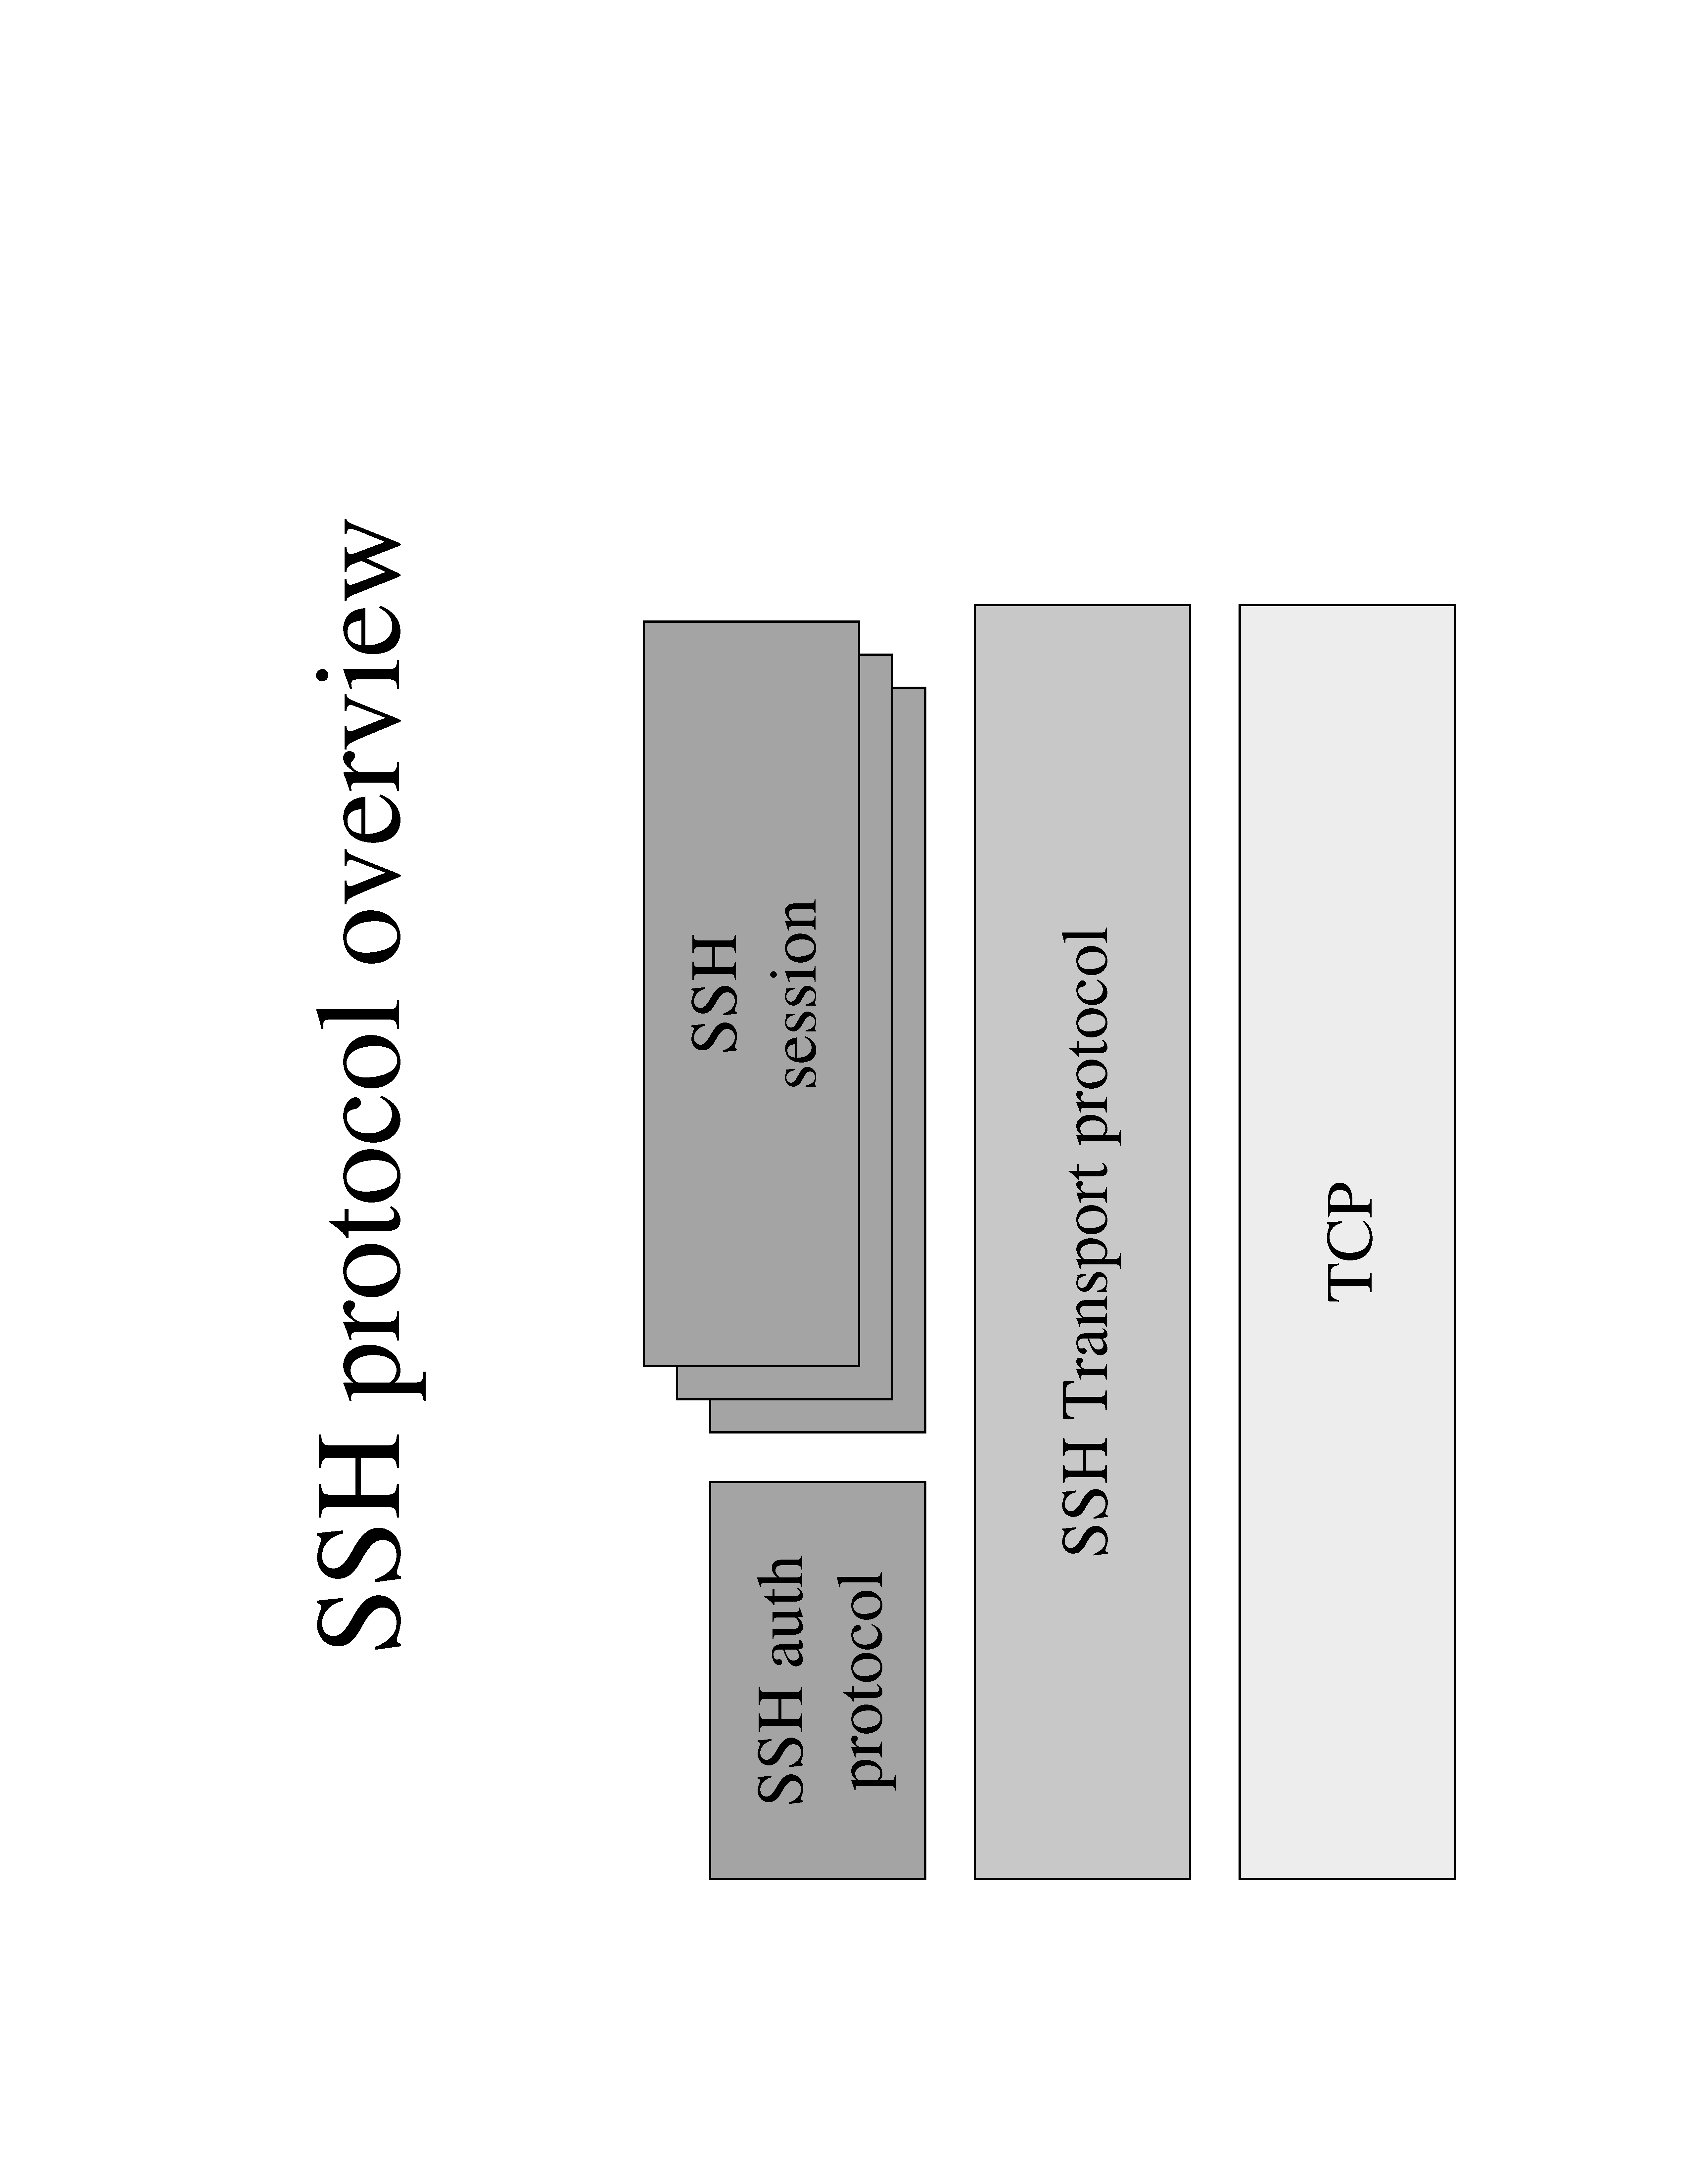
\includegraphics[clip,scale=0.4,angle=270]{ssh_overview}

\caption{\label{fig:ssh-overview} protocol hierarchy}

\end{figure}



\subsubsection{Session Initialization}

The initial handshake provides the client and server with an
opportunity to \textit{1)} perform a key exchange, \textit{(2)}
validate the server key, and \textit{(3)} negotiate an initial set of
cryptographic algorithms that will be used for the session (e.g. for
cipher, HMAC). An overview of the handshake messages are shown in
\ref{fig:ssh-init}. The steps of the protocol are as follows.  Refer
to Figure \ref{fig:ssh2-init} for details.
\begin{enumerate}
\item The SSH server sends a string of the form
  {}``SSH-2.0-\emph{software}''.  The \emph{software} string
  identifies the particular client or server.  (as a variation, it may
  also send SSH-1.99-\emph{software''} to indicate protocol version 1
  compatibility) For example, the OpenSSH 4.5 software sends
  {}``SSH-1.99-OpenSSH\_4.5''. If the client does not understand the
  protocol version, it disconnects, otherwise it sends a similar
  string to the server. After these strings are sent, all traffic uses
  the binary packet protocol shown in Figure \ref{fig:ssh-packet}.\\
%
\begin{figure}
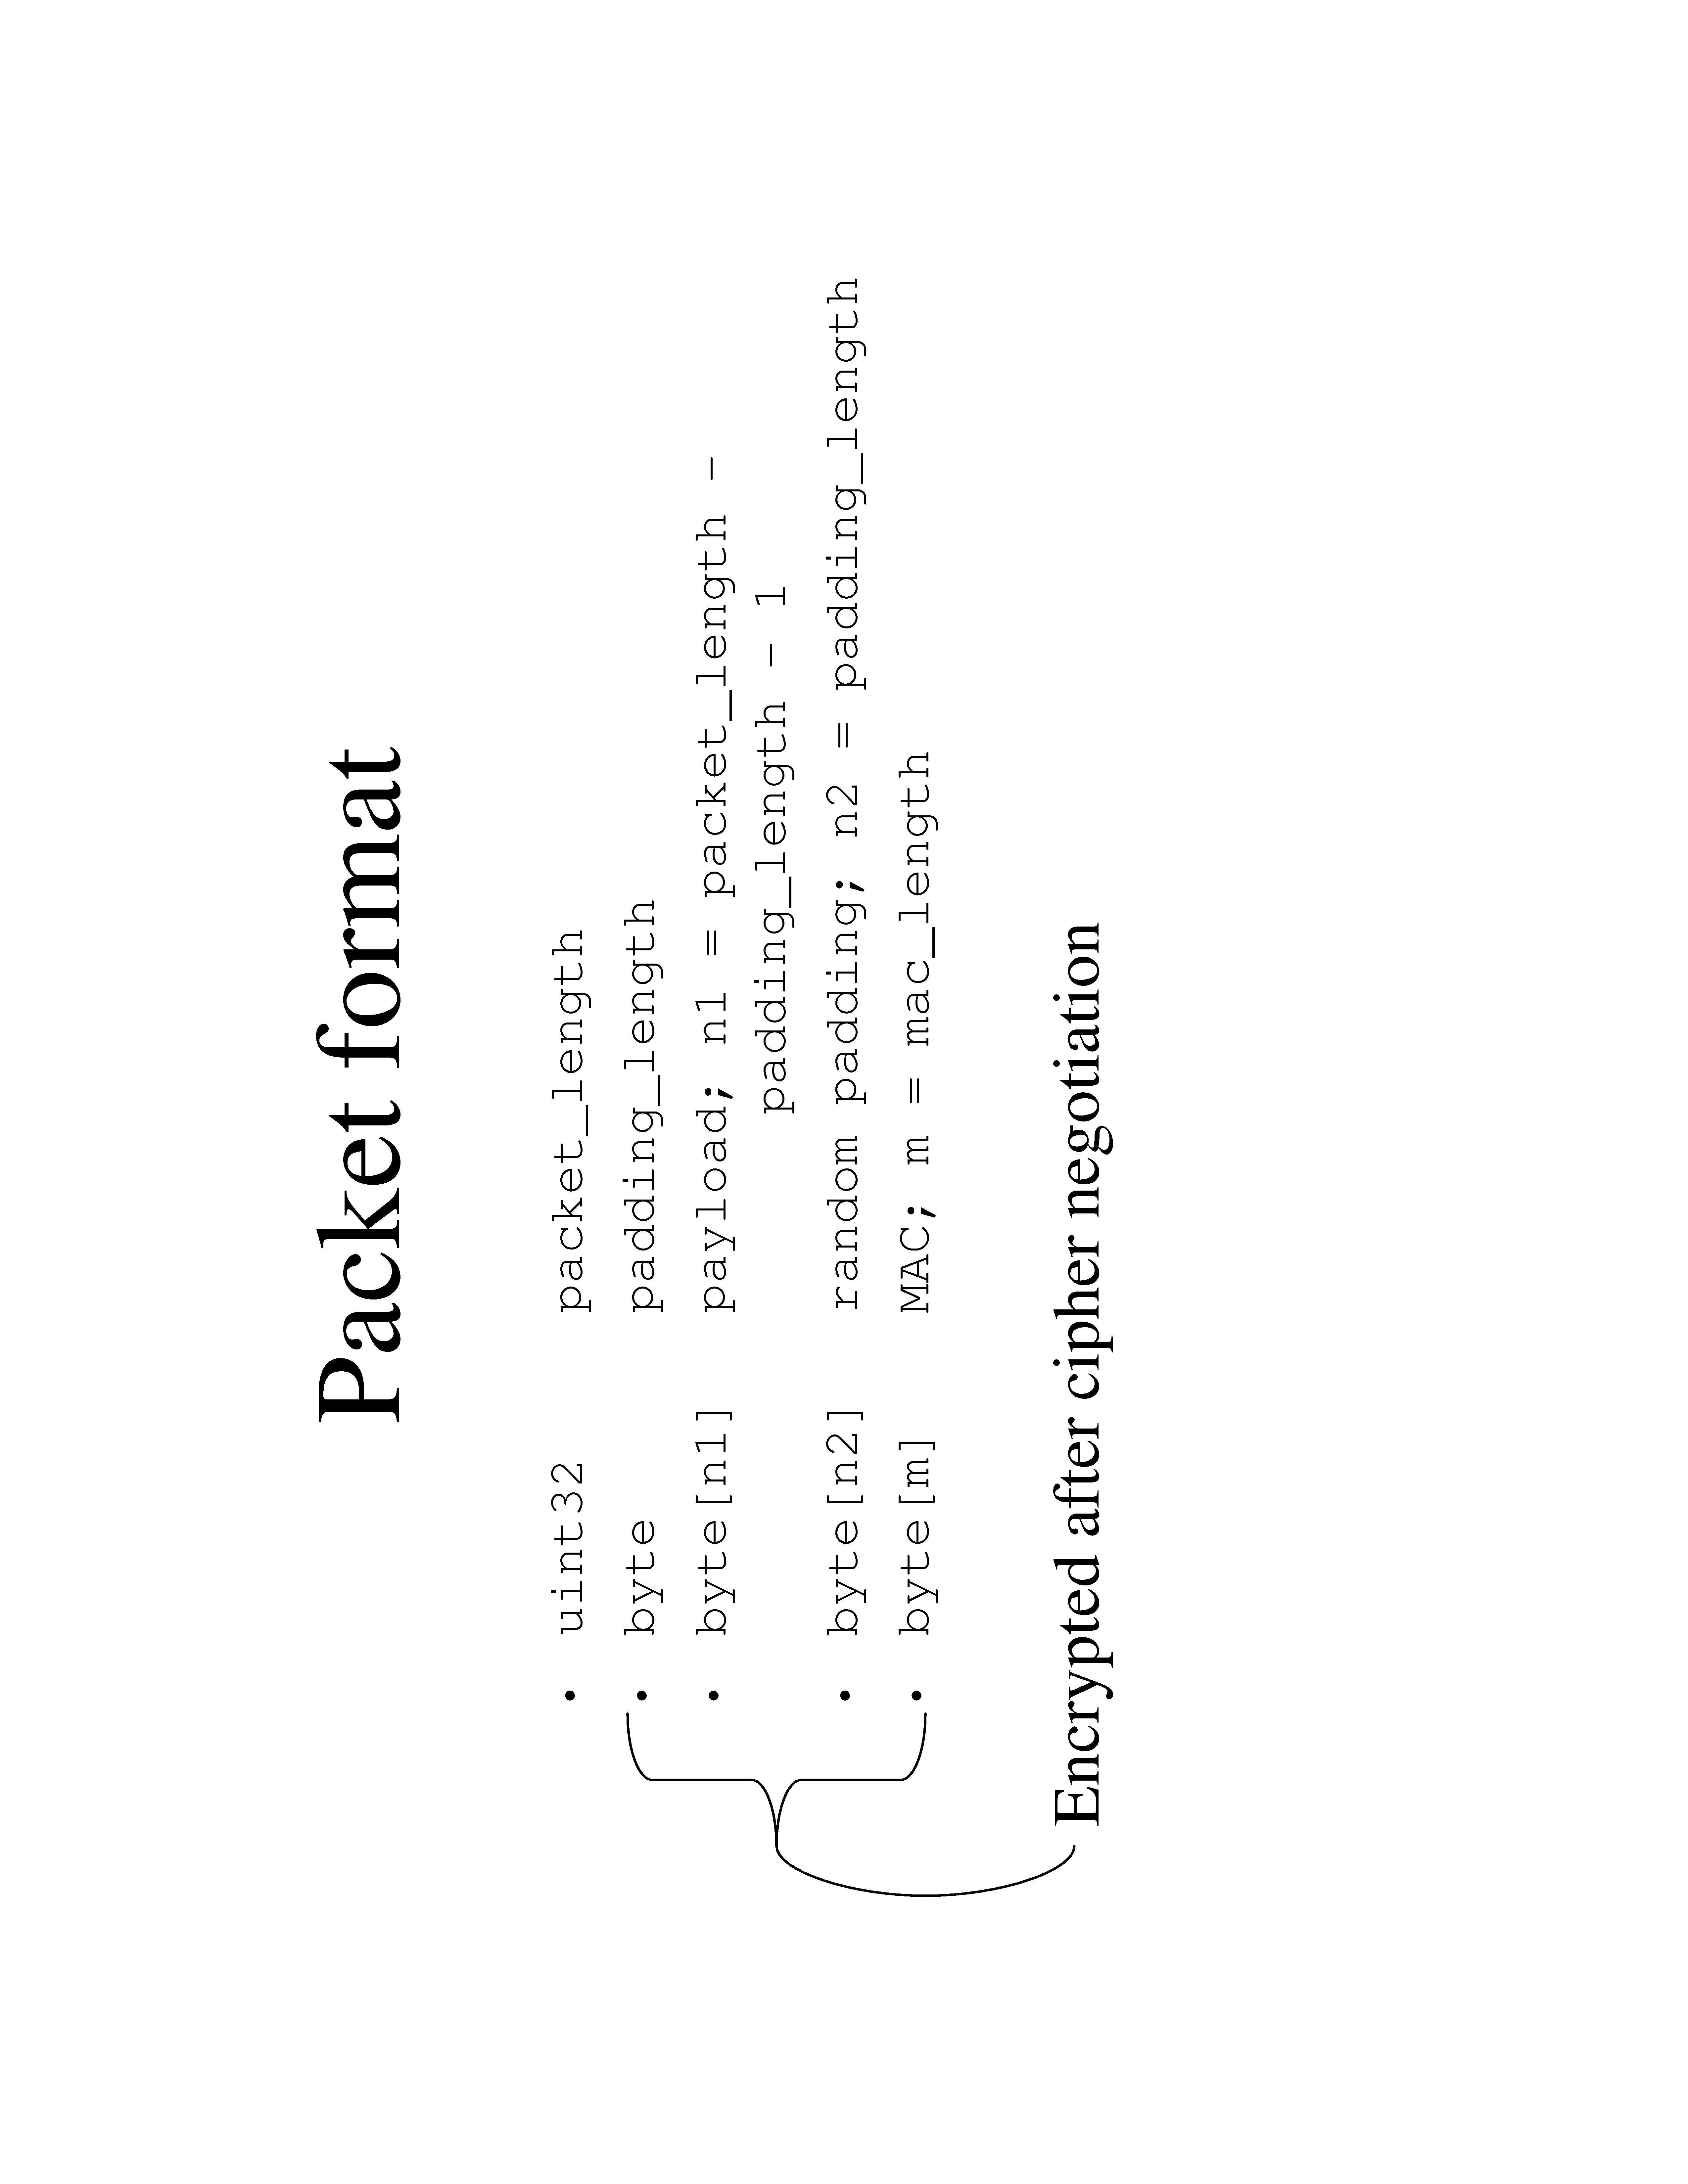
\includegraphics[clip,scale=0.4,angle=270]{ssh_packet}

\caption{\label{fig:ssh-packet} binary packet structure}

\end{figure}

\item Each party sends an SSH\_MSG\_KEXINIT message to begin the key exchange.
This message includes a list of supported ciphers, HMAC algorithms,
compression algorithms, and key exchange algorithms, ranked by preference.
For each algorithm, the parties choose the highest preference algorithm
of the client, which is also supported by the server. If one of the
algorithm lists has no algorithm in common, the connection is terminated.
%% The format of the SSH\_MSG\_KEXINIT message are as follows:

%% \begin{lyxcode}
%% ~~~~~~byte~~~~~~~~~SSH\_MSG\_KEXINIT

%% ~~~~~~byte{[}16{]}~~~~~cookie~(random~bytes)

%% ~~~~~~name-list~~~~kex\_algorithms

%% ~~~~~~name-list~~~~server\_host\_key\_algorithms

%% ~~~~~~name-list~~~~encryption\_algorithms\_client\_to\_server

%% ~~~~~~name-list~~~~encryption\_algorithms\_server\_to\_client

%% ~~~~~~name-list~~~~mac\_algorithms\_client\_to\_server

%% ~~~~~~name-list~~~~mac\_algorithms\_server\_to\_client

%% ~~~~~~name-list~~~~compression\_algorithms\_client\_to\_server

%% ~~~~~~name-list~~~~compression\_algorithms\_server\_to\_client

%% ~~~~~~name-list~~~~languages\_client\_to\_server

%% ~~~~~~name-list~~~~languages\_server\_to\_client

%% ~~~~~~boolean~~~~~~first\_kex\_packet\_follows

%% ~~~~~~uint32~~~~~~~0~(reserved~for~future~extension)
%% \end{lyxcode}
%
\begin{figure}
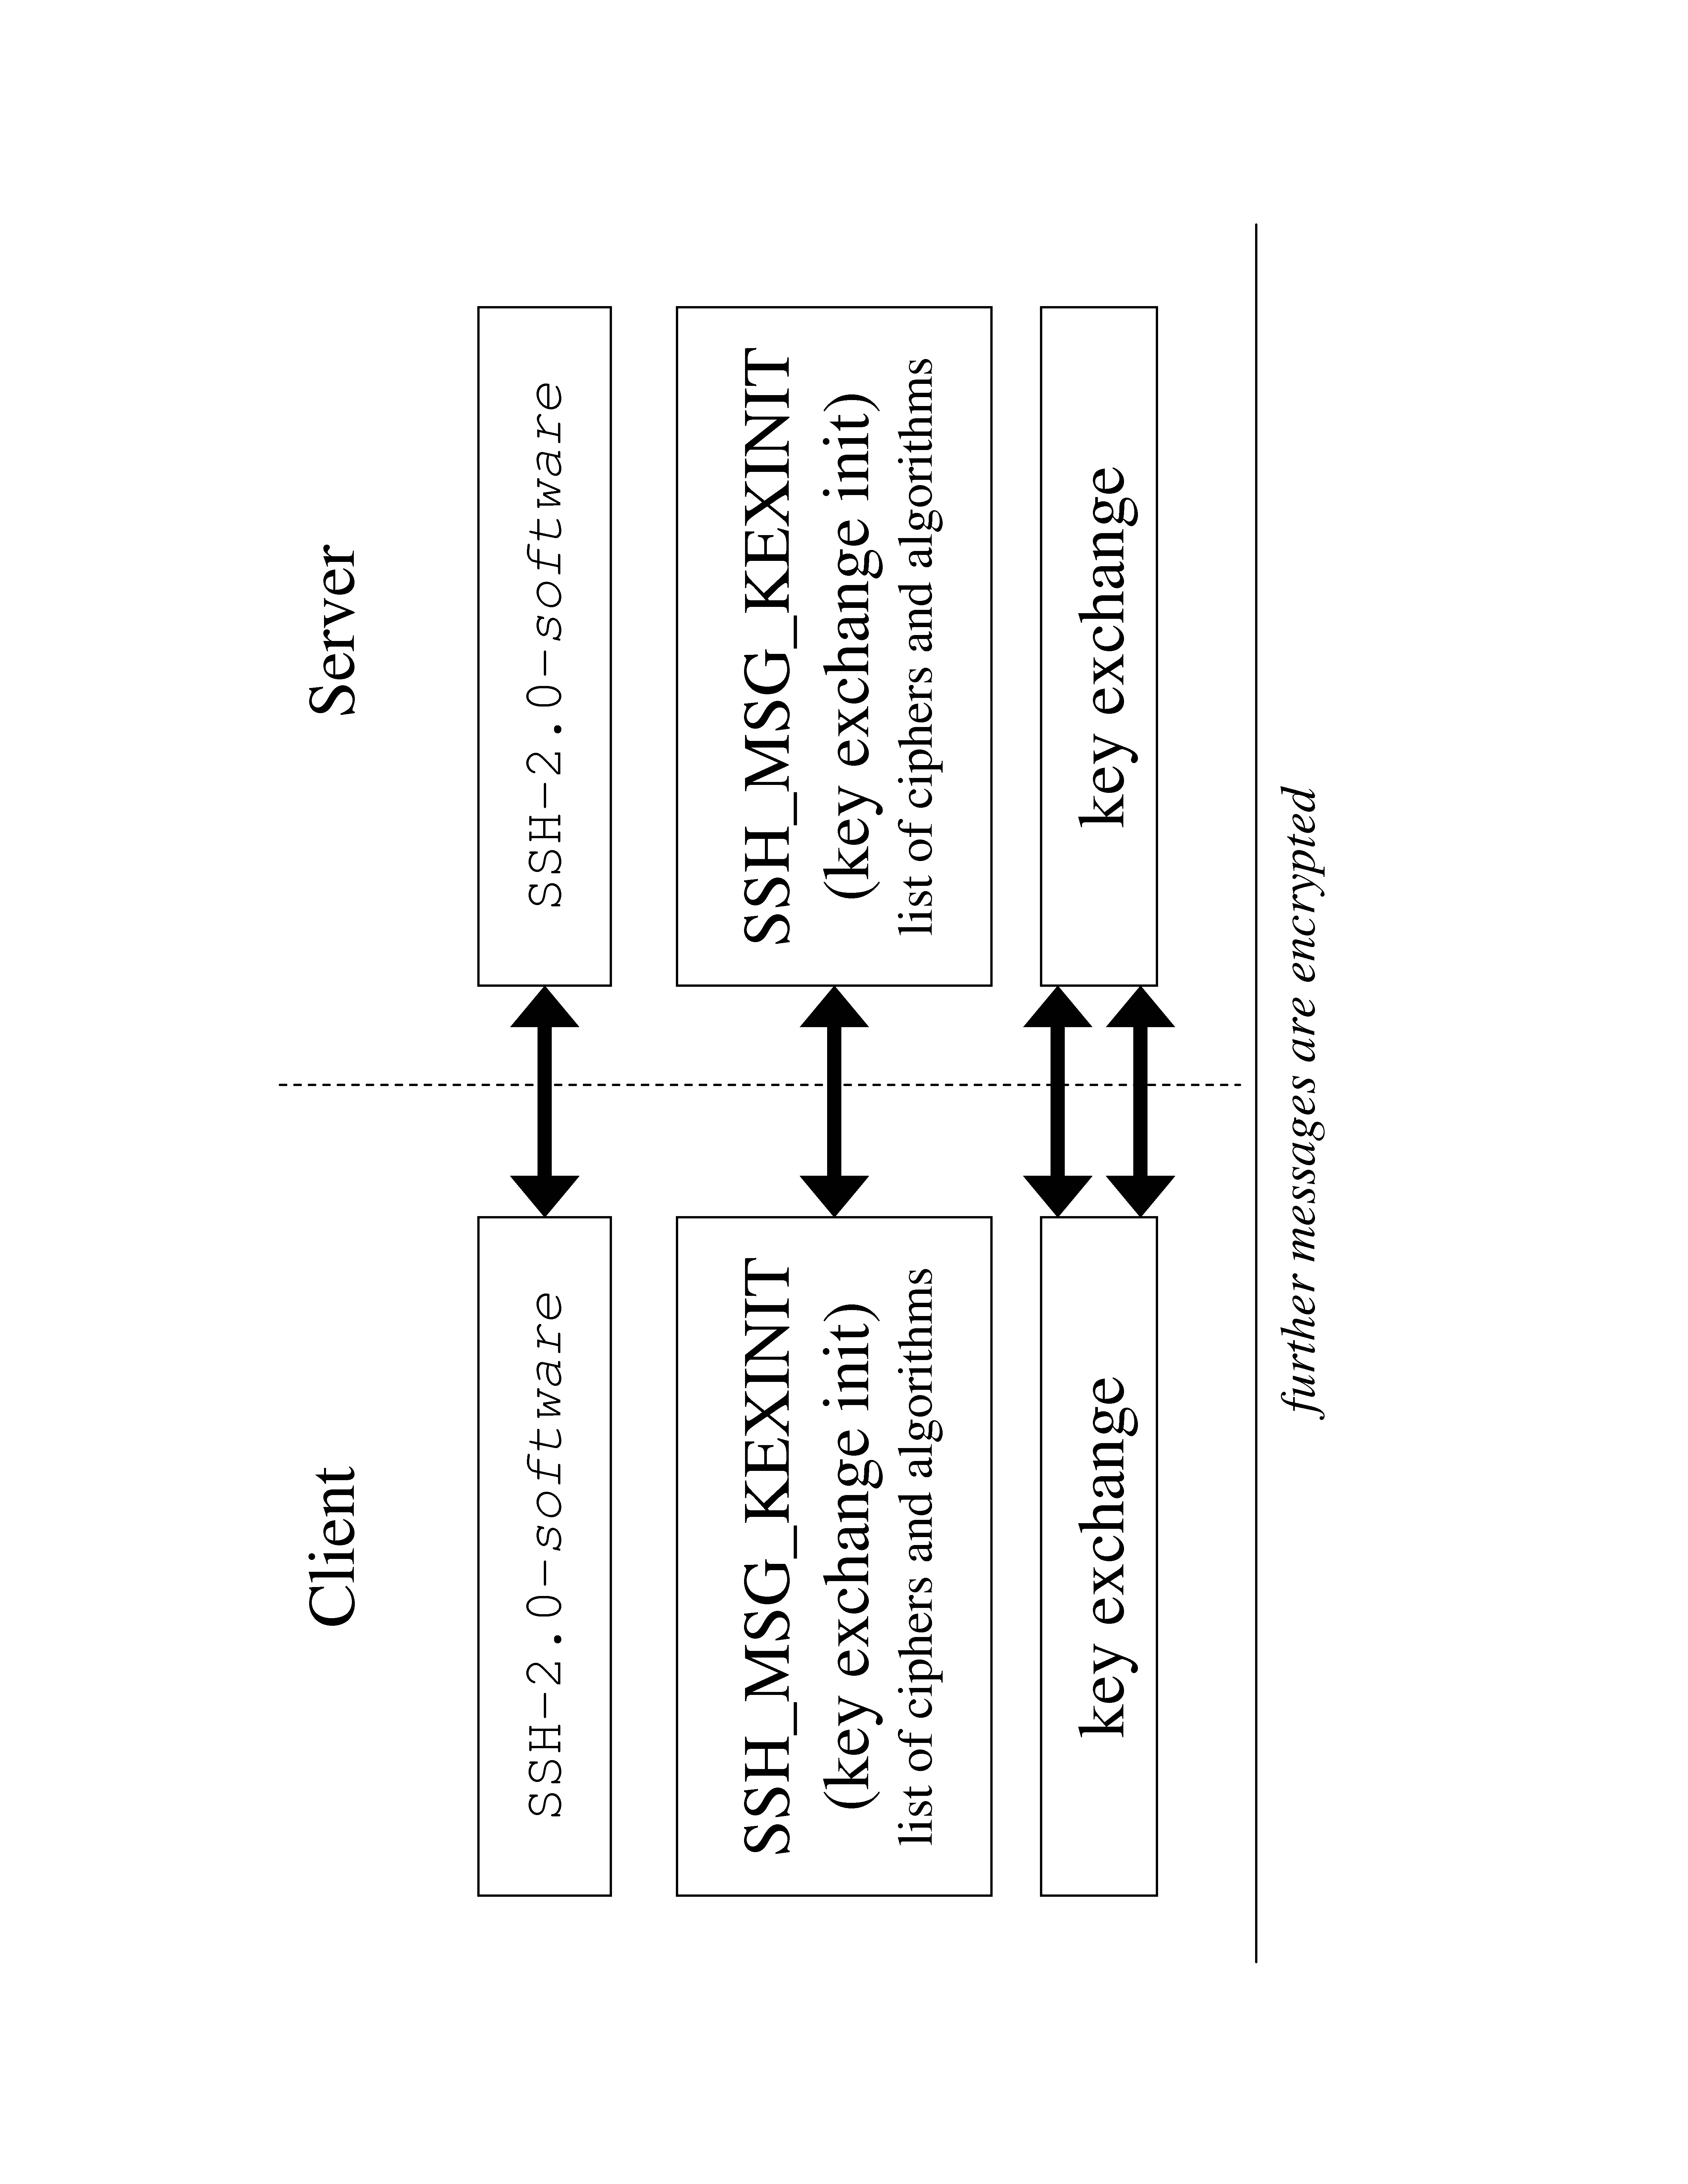
\includegraphics[clip,scale=0.4,angle=270]{ssh_init}

\caption{\label{fig:ssh-init} connection handshake protocol}

\end{figure}


%
\begin{figure}[t]
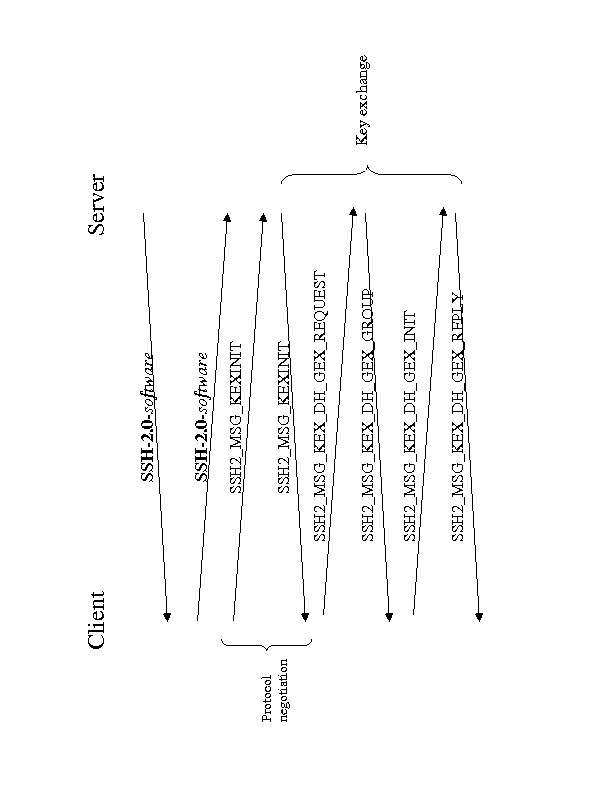
\includegraphics[clip,scale=0.4,angle=270]{ssh2_p1}

\caption{\label{fig:ssh2-init} connection handshake protocol}

\end{figure}


\item Following the handshake, the key exchange protocol is performed. The
specific algorithm used to do the key exchange is negotiated in the
previous step. The original SSH2 specification included a single Diffie-Hellman
group defined in \cite{rfc4253}. A newer and more flexible key exchange
algorithm is defined in \cite{rfc4419}. The details of key exchange
will not be discussed further. After the key exchange is complete,
all of the data in the SSH stream is encrypted using the negotiated
cipher and key. Specifically, the sequence of packets, excluding the
packet size header, shown in \ref{fig:ssh-packet} is a single stream
of plaintext encrypted by the cipher.
\end{enumerate}
At this point, the protocol handshake is complete and the client may
initiate arbitrary sub-protocols of SSH. Typically, the client will
begin the client authentication protocol, as most servers require
authentication before allowing other services to be used.


\subsubsection{Client Authentication}

When the initial handshake is complete, the client has verified the
server key, if possible, but the client has not yet authenticated to
the server. The SSH auth protocol~\cite{rfc4252} can be initiated to
perform this. The auth protocol is flexible; the SSH standard
describes several commonly-used methods of authentication, such as
password and public-key, but arbitrary authentication methods can be
added. The client selects the desired method of authentication among
those supported by the server.

The messages used in password authentication are shown in
\ref{fig:ssh-auth}.  For the purposes of this discussion, we will
assume the client is using the {}``password'' authentication
method. The steps of this authentication are as follows:
\begin{enumerate}
\item The client sends the username and password to the server in an
  SSH\_MSG\_USERAUTH\_REQUEST message. 

%% The format of this message is:

%% \begin{lyxcode}
%% ~~~~~~byte~~~~~~SSH\_MSG\_USERAUTH\_REQUEST

%% ~~~~~~string~~~~user~name~in~ISO-10646~UTF-8~encoding~{[}RFC3629{]}

%% ~~~~~~string~~~~\textquotedbl{}password\textquotedbl{}

%% ~~~~~~boolean~~~FALSE

%% ~~~~~~string~~~~plaintext~password~in~ISO-10646~UTF-8~encoding~


%% \end{lyxcode}
\item If the server does not support the {}``password'' method chosen,
or the password is incorrect, the server will respond with an SSH\_MSG\_USERAUTH\_FAILURE
message. If the password is correct, the server sends a SSH\_MSG\_USERAUTH\_SUCCESS
message, and the client may begin requesting services. (The server
may also send a SSH\_MSG\_USERAUTH\_BANNER packet to communicate information
directly to the user. It is analogous to the /etc/issue file used
in standard Unix systems to display a message at a login prompt)
\end{enumerate}
%
\begin{figure}
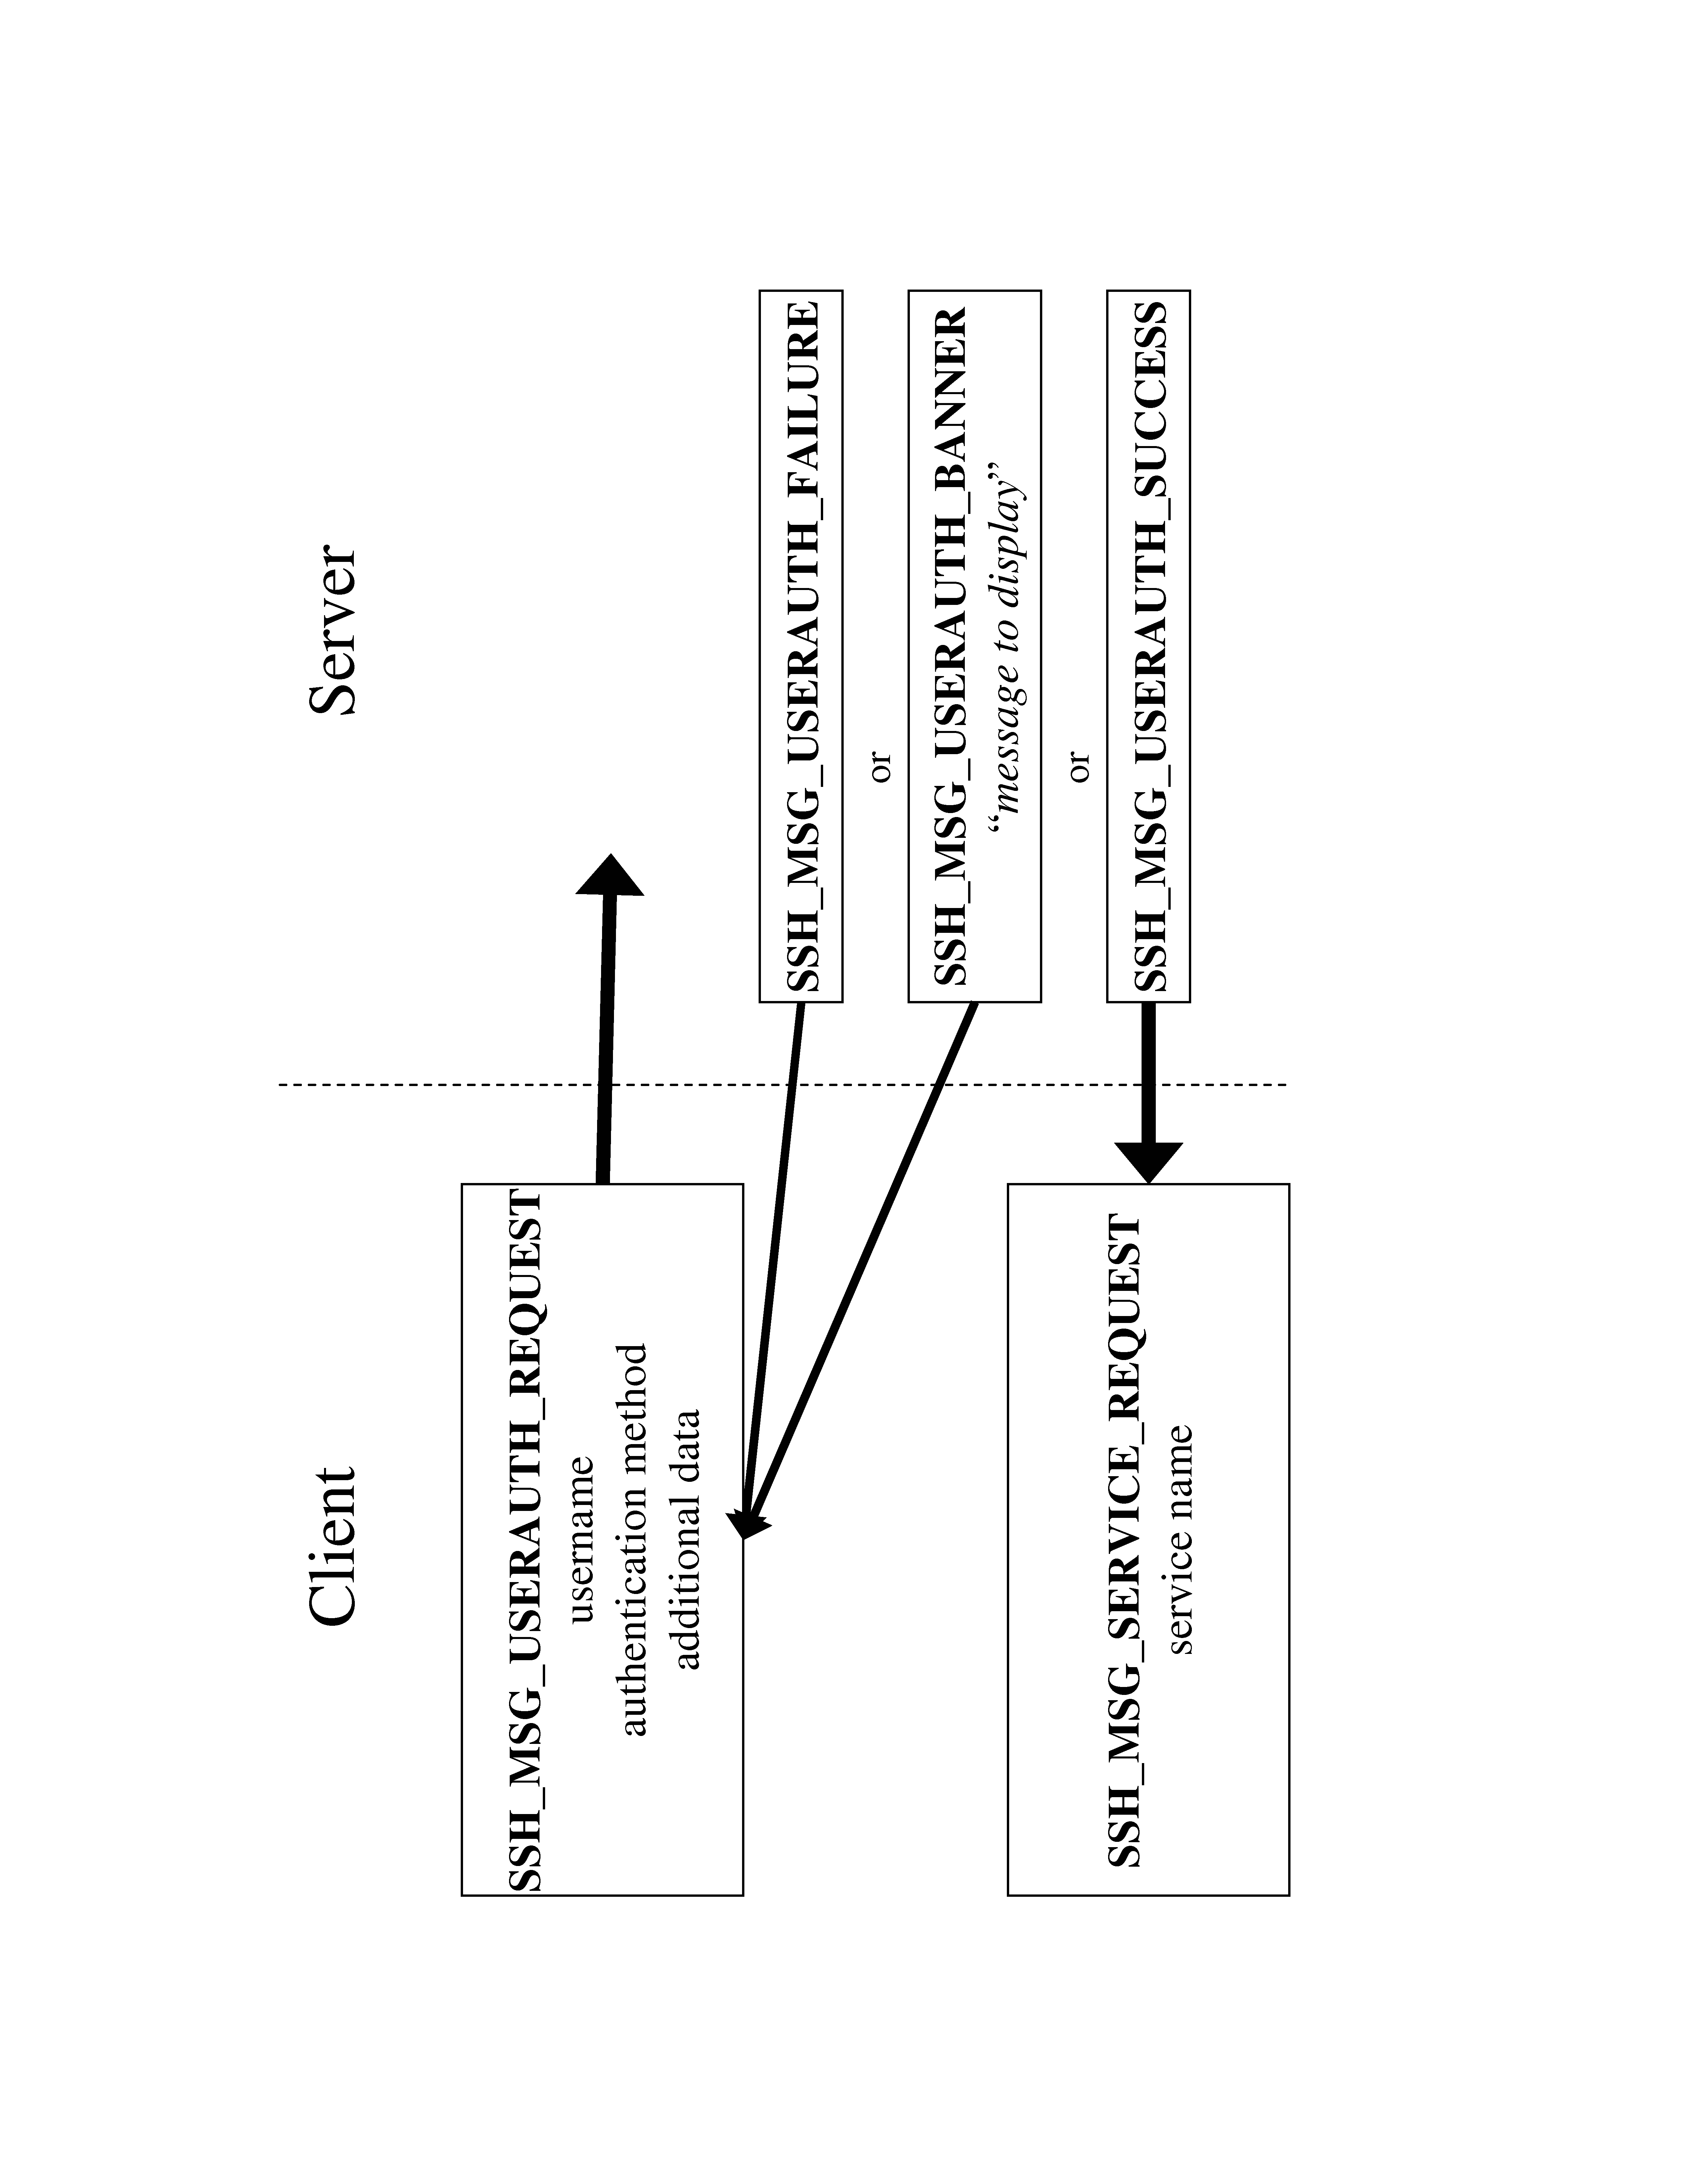
\includegraphics[clip,scale=0.4,angle=270]{ssh_auth}

\caption{\label{fig:ssh-auth} authentication protocol messages}

\end{figure}


The password is sent directly from the client to the server in a
packet. Thus, the only protection from eavesdroppers is the encryption
applied at the SSH transport layer. There is no protection of the
client's authentication credentials from the server itself, so if the
server is malicious or has been compromised, an attacker will learn
everything the client sends, and can potentially impersonate the
client at another time.


\subsection{Man in the Middle Attack}

As mentioned in the overview, as well as the previous section, the SSH
protocol is vulnerable to password compromise. An attacker can exploit
the insecurity of password transmission by mounting a \emph{man in the
  middle} (MITM) attack. Although the protocol does provide some
protection against MITM in the form of host key authentication, there
are several ways in which an attacker can thrwart this protection:
\begin{enumerate}
\item If the attacker manages to steal the host key, then the attacker can
successfully impersonate the server without detection. There is no
other means for the client to authenticate the server.
\item If the client does not know the server's host key, then the host
  cannot be authenticated unless the client has an alternative trusted
  channel to validate the host key. As mentioned in the overview, the
  following message is typically displayed by the OpenSSH client when
  connecting to a server with an unknown key\\
%
\begin{minipage}[t]{1\columnwidth}%
\begin{lyxcode}


The~authenticity~of~host~'server~(1.2.3.4)'~can't~be~established.

RSA~key~fingerprint~is~3f:76:22:43:c2:03:b9:71:b0:31:ce:87:37:45:cb:02.~

Are~you~sure~you~want~to~continue~connecting~(yes/no)?
\end{lyxcode}
%
\end{minipage}\\

Practically speaking, it may be inconvenient for a user to authenticate
the server using this message and make a correct decision. It is easy
to imagine a user simply answering yes in order to bypass the inconvenience. 
\item Even if the client does know the server's key, the there is no
  guarantee that a user would refuse to connect even if the
  authentication fails. In fact, there are several reasonable
  explanations for why a user may choose to accept a failed
  authentication and continue with the connection. For example, the
  user might think the server key changed for a non-malicious reason
  such as an operating system upgrade where the administrator forgot
  to backup the old key.
\end{enumerate}

While the only method that guarantees the success of the attacker is
\textit{(1)}, each poses a real security problem for users of SSH.

\subsection{SPAKA using SFE}

As previously hinted, this vulnerability can be mitigated by using
additional secrets which are shared between the client and server. The
password is a convenient shared secret already in common use
today. Typically, a password is considered only as a means of
authenticating a client to a server, but with certain protocols a
password can also be used for simultaneous mutual authentication in a
way that is secure, and does not compromise the password if the server
is malicious. Such protocols are known as \emph{secure password and
  key authentication} (SPAKA).

It is important to note that a {}``password'' need not be a constant
string that the user remembers over a long period of time, it can be
any string that serves as a mutual authenticator. For example, secure
ID tokens that display constantly changing strings, time synchronized
with the server, are considered to be a more secure alternative to
traditional passwords, such alternatives are readily usable in SPAKA
protocols.

The design of previous SPAKA protocols~\cite{brainard03} suggests that
SFE can be applied generally to the SPAKA problem. Here is a general
SPAKA construction based on SFE:

\begin{enumerate}

\item Let $X$ be the user's password, $Y=H(X)$ be a hash of $X$.

\item Let $C$ be the client and $S$ be the server. $C$ and $S$ participate
in a secure evaluation of the following function $f$, where $C$
provides input $X$ and $S$ provides input $Y$. $C$ and $S$ both
receive the same output from $f$, which is a single bit denoting a
boolean value.
\[
f(X,Y)=_{def} \left(Y=H\left(X\right)\right)
\]
If the value of the $f$ is $false$ then it is evident that one of the
parties did not possess the shared secret, and the mutual
authentication fails. Otherwise the mutual authentication succeeds.

\end{enumerate}

Notice that $f$ is nothing more than a variant of the well-known
millionaire problem, where the relational predicate used is equality
rather than less than or greater than. If $f$ is evaluated securely,
then $C$ and $S$ are guaranteed not to learn any information about the
computation except for the single bit of output, thus allowing them
mutual authentication without revealing any information to potential
attackers. This authentication scheme can be integrated into
implementations of the SSH protocol trivially to provide protection
from the MITM attack previously described.

%
\begin{comment}
\begin{enumerate}
\item Practical SSH paper
\item New protocol paper
\item Theoretical paper
\item Graduate!!!
\end{enumerate}

\end{comment}
{}


\section{Implementation}

We implemented an SSH client and server that incorporate this SPAKA
protocol. The following components were used:
\begin{enumerate}
\item The Dropbear SSH client and server. We chose to use this client
because of it's small and simple codebase.
\item The SFE-Tools secure function evaluation compiler first described
by Kruger \textit{et al.}
\end{enumerate}
A new authentication method was defined in the client and server code
using the extensible SSH architecture. To initiate the SPAKA
authentication protocol, the client sends an authorization protocol
request:
\begin{lyxcode}
~~~~~~byte~~~~~~SSH\_MSG\_USERAUTH\_REQUEST

~~~~~~string~~~~username

~~~~~~string~~~~\textquotedbl{}sfeauth\textquotedbl{}

~~~~~~boolean~~~FALSE
\end{lyxcode}
The server responds with the type of password hashing used to store
passwords on this system. Examples include {}``DES'' for the traditional
UNIX password crypt function, and {}``MD5'' for the default password
hashing algorithm used on most modern Linux systems. 
\begin{lyxcode}
~~~~~~byte~~~~~~SSH\_MSG\_USERAUTH\_RESPONSE

~~~~~~string~~~~username

~~~~~~string~~~~\textquotedbl{}MD5\textquotedbl{}

~~~~~~boolean~~~FALSE
\end{lyxcode}
After this exchange, the client prepares an encrypted circuit corresponding
to the hashing method in use. The underlying SFE protocol runs, wrapped
inside SSH messages SSH\_MSG\_USERAUTH\_MSG1 and SSH\_MSG\_USERAUTH\_MSG2.

\section{Related Work}

\subsection{SPAKA}

\emph{Secure Password and Key Authentication} (SPAKA) is a class of
authentication protocols first described in \cite{bellovin92}. SPAKA
protocols are designed to guarentee confidentiality of secrets even
against active adversaries. There have been various SPAKA protocols
proposed in the literature with varying properties. A recent SPAKA
protocol is presented in \cite{brainard03}. In this protocol, the
user's password $P$ is split into two shares: $P_{1}$ and $P_{2}$.
The value of $P$ can not be derived from either of the two shares
alone, and each share is stored on a seperate server. To perform the
protocol, the client splits $P$ into different shares $P_{1}'$ and
$P_{2}'$, and sends these values to the servers. The servers then
perform an evaluation protocol to determine if $P_{1}\oplus P_{2}=P_{1}'\oplus P_{2}'$.

\bibliographystyle{plain}
\bibliography{somesh,ssh}

\end{document}



\part{Timeline}


\subsection{Summer 2007}
\begin{itemize}
\item Secure authentication in SSH (see section \ref{sub:SPAKA-using-SFE})

\begin{itemize}
\item define protocol extension
\item implement classic SPAKA 
\item implement SFE SPAKA
\item benchmark and compare
\end{itemize}
\item Target publication: Usenix Security 2008
\end{itemize}

\subsection{Fall 2007}
\begin{itemize}
\item Investigate optimizations of cryptographic primitives (see section
\ref{sub:Other-Optimizations})

\begin{itemize}
\item adapt standard oblivious transfer algorithms to use more efficient
representations, such as elliptic curve groups
\item evaluate modular square root oblivious transfer (see section \ref{sec:OT-SquareRoots})
\item investigate use of other kinds of functions for oblivious transfers
and homomorphic encryption
\end{itemize}
\item Target publication: TBD
\end{itemize}

\subsection{Winter/Spring 2008}
\begin{itemize}
\item Investigate use of other circuit representations (see section \ref{OBDD-section})

\begin{itemize}
\item evaluate which OBDD extensions are good candidates for secure protocols
\item implement compiler and protocols
\item performance measurements
\end{itemize}
\item Target publication: TBD
\end{itemize}

\subsection{Spring/Summer 2008}
\begin{itemize}
\item Investigate optimizations resulting from controlled leakage of information.
(see section \ref{sub:Other-Optimizations})

\begin{itemize}
\item Develop specification language to tag intermediate values as sensitive
or non-sensitive
\item Develop hybrid evaluation protocols that protect sensitive data but
avoid the overhead when evaluating non-sensitive computations
\item Implement and measure performance gains
\end{itemize}
\end{itemize}

\subsection{Fall/Winter 2008}
\begin{itemize}
\item Optimizing protocol compiler. (see section \ref{sub:An-Efficient-Framework})

\begin{itemize}
\item Define programming language for expressing secure computations

\begin{itemize}
\item Language will include direct support for common SFE techniques, such
as homomorphic encryption, and metadata for privacy levels
\end{itemize}
\item Implement compiler for this language into securely evaluable {}``machine
code''
\item Automatic optimizer will try different representations of the functions,
including OBDDs, Boolean circuits, and other ideas from my research,
and produce as efficient as a representation as possible
\item Implement protocol evaluation library, to make straightforward use
in ordinary applications.
\end{itemize}
\end{itemize}

\subsection{Spring 2009}
\begin{itemize}
\item Write dissertation and graduate.
\end{itemize}



\bibliographystyle{plain}
\bibliography{privacy,somesh,ssh,crypto}

\end{document}

%\chapter{Futher Analysis}

Lorem ipsum dolor sit amet, consectetur adipisicing elit, sed do eiusmod tempor incididunt ut labore et dolore magna aliqua. Ut enim ad minim veniam, quis nostrud exercitation ullamco laboris nisi ut aliquip ex ea commodo consequat. Duis aute irure dolor in reprehenderit in voluptate velit esse cillum dolore eu fugiat nulla pariatur. Excepteur sint occaecat cupidatat non proident, sunt in culpa qui officia deserunt mollit anim id est laborum.

\section{The First}

Lorem ipsum dolor sit amet, consectetur adipisicing elit, sed do eiusmod tempor incididunt ut labore et dolore magna aliqua. Ut enim ad minim veniam, quis nostrud exercitation ullamco laboris nisi ut aliquip ex ea commodo consequat. Duis aute irure dolor in reprehenderit in voluptate velit esse cillum dolore eu fugiat nulla pariatur. Excepteur sint occaecat cupidatat non proident, sunt in culpa qui officia deserunt mollit anim id est laborum.

Lorem ipsum dolor sit amet, consectetur adipisicing elit, sed do eiusmod tempor incididunt ut labore et dolore magna aliqua. Ut enim ad minim veniam, quis nostrud exercitation ullamco laboris nisi ut aliquip ex ea commodo consequat. Duis aute irure dolor in reprehenderit in voluptate velit esse cillum dolore eu fugiat nulla pariatur. Excepteur sint occaecat cupidatat non proident, sunt in culpa qui officia deserunt mollit anim id est laborum.


\subsection{The Second}

Lorem ipsum dolor sit amet, consectetur adipisicing elit, sed do eiusmod tempor incididunt ut labore et dolore magna aliqua. Ut enim ad minim veniam, quis nostrud exercitation ullamco laboris nisi ut aliquip ex ea commodo consequat. Duis aute irure dolor in reprehenderit in voluptate velit esse cillum dolore eu fugiat nulla pariatur. Excepteur sint occaecat cupidatat non proident, sunt in culpa qui officia deserunt mollit anim id est laborum.

Lorem ipsum dolor sit amet, consectetur adipisicing elit, sed do eiusmod tempor incididunt ut labore et dolore magna aliqua. Ut enim ad minim veniam, quis nostrud exercitation ullamco laboris nisi ut aliquip ex ea commodo consequat. Duis aute irure dolor in reprehenderit in voluptate velit esse cillum dolore eu fugiat nulla pariatur. Excepteur sint occaecat cupidatat non proident, sunt in culpa qui officia deserunt mollit anim id est laborum.


%%%%%%%% TABLE %%%%%%%%
\begin{table}[t]
\caption[Short caption for list-of-tables]{Full-length caption for the actual thesis text.}
\vspace{1em}
\footnotesize
\begin{center}
    \begin{tabular}{|l|c|c|c|}
    \hline
    \textbf{One Potato} & \textbf{Two Potato} & \textbf{Three Potato} & \textbf{Four} \\
    \hline
    Russet & 2.0 & 0.33 & iv \\
    \hline
    \end{tabular}
\end{center}
\label{tab:table}
\end{table}

\chapter{Introduction}
\begin{quote}
%
\begin{comment}
\begin{quote}
As every man goes through life he fills in a number of forms for the
record, each containing a number of questions... There are thus hundreds
of little threads radiating from every man, millions of threads in
all. If these threads were suddenly to become visible, the whole sky
would look like a spider's web, and if they materialized as rubber
bands, buses; trams and even people would all lose the ability to
move, and the wind would be unable to carry torn-up newspapers or
autumn leaves along the streets of the city. They are not visible,
they are not material, but every man is constantly aware of their
existence.... Each man, permanently aware of his own invisible threads,
naturally develops a respect for the people who manipulate the threads.

--Alexander Solzhenitsyn, Cancer Ward, 1968.
\end{quote}

\end{comment}
{}
\end{quote}
Privacy and security are important concerns as computers increase
in power and the Internet continues to grow \cite{cra99,tur03}. Everyday
activities dealing with sensitive data are moving onto to the Internet,
such as credit card transactions, doctors accessing medical records,
and online banking. As a result, more data is stored on machines that
are connected to the Internet, directly or indirectly, then ever before.
Sadly, there are many all-too-common examples in the news of
privacy compromising activities such as phishing, data theft, and
identity theft. New techniques are needed to deal with the many threats
to privacy. In addition to the misuse of data, there can be other
consequences of privacy violations, such as serious legal penalties
for violation of HIPAA laws \cite{hippa}, which mandate strict privacy
requirements among health-care professionals.

Despite these many privacy concerns, there is also a conflicting desire
to perform useful computations with sensitive data. Data is not useful
unless it can be accessed and manipulated. Sometimes various parties
would like to collaborate on research involving this data. For
example, genetic data is the subject of much current research, but
it is considered private personal information. Researchers with access
to different patients' data may want to combine their information
resources in the search for new cures for diseases, without revealing
the actual sensitive information to the collaborating parties. Competing
businesses may want to jointly perform market research for mutual
benefit, without exposing their sensitive business data. Therefore,
the challenge
is how to balance these competing concerns, making data available
for desirable uses while preserving as much privacy as possible.  By
providing strong privacy guarentees, we enable new uses of sensitive data.

These concerns are not merely theoretical. In 2000, Ford Motor Explorer
SUVs had a well publicized problem with their Firestone tires, in
which the tire treads could fail under certain circumstances. At least
271 deaths resulted \cite{NYTFordFirestone}. The problem resulted
from the \emph{combination} of products: There were no problems with
the same tires in other vehicles, nor with Ford Explorers using other
tires. It has been suggested that the crisis could have been averted
using joint data-mining, however, due to business secrecy concerns,
such research could only have been done using privacy preserving methods
\cite{VaidyaClifton:2002}.

There have been several methods developed so far for preserving personal
privacy while permitting use of data. The most simple method, conceptually,
is to replace identifying information, such as the name, social security
number, and other sensitive data with random unique identifiers, and
then using the transformed data for computation. If it is necessary
to correlate the outputs of the computation with individuals, the
data owner can do this, but other parties presumably can not. However,
this method has been shown to be vulnerable to attacks that correlate
the transformed data with information available from external sources
to reconstruct the obfuscated data, thereby breaking the privacy protection
\cite{Malin04}. 

Another method for preserving privacy is known as \emph{secure multiparty
computation}\cite{Yao86}. This is a technique of performing computations on inputs
supplied by multiple parties while provably maintaining privacy guarantees.
If the computation is a function evaluation, then it is called \emph{secure
function evaluation}, or SFE. This is a technique which in theory can address
many of the privacy concerns we face. The inputs to
the function are partitioned among more than one party, and the function
is computed collaboratively while preserving the privacy of each participant's
individual inputs. In this case, privacy is considered preserved if
no party learns any information that would affect their estimate of
the probability distribution of another party's inputs, except for
that which can be calculated by the parties' own inputs and the output
of the joint function. In comparison with other methods, only secure
multiparty computation can be used to guarantee privacy when parties
collaborate on joint computation. %
\begin{comment}
%
\begin{lyxgreyedout}
Needs clarification
\end{lyxgreyedout}
 In other words, the entropy gain of each party is equivalent to the
entropy gain in an idealized protocol where a trusted third party
collects all the inputs, evaluates the function, and transmits only
the output to each party. Depending on the protocol, the guarantees
for some parties may be based on typical assumptions of computational
hardness, while the guarantees for other parties may be information
theoretic.
\end{comment}
{}

Although SFE has provable privacy guarantees, its implementation tends
to be very expensive for practical use in terms of time and space.
The space expense manifests itself in the large consumption of network
bandwidth used in the protocols, and the time expense comes from repeated
use of expensive cryptographic primitives, such as modular exponentiation.
These expenses explain why SFE has not been frequently used outside
of the academic literature, despite the fact that it was formally
introduced in the literature in the early 1980s \cite{Y82}. There has
been research in recent years to make SFE more practical. This research
falls into two categories: general and function specific. General
protocols allow any function expressed as a circuit computation to
be evaluated securely. The Fairplay system \cite{Fairplay} is a straightforward
implementation of the Yao protocol \cite{Yao86}, presented in section
\ref{sub:Garbled-Circuit-Method}, along with a supporting compiler
that allows secure functions to be written in a more familiar functional
programming notation. We showed
how \emph{Ordered Binary Decision Diagrams} (OBDD)  can be used to
produce a more efficient protocol for secure evaluation for certain
functions\cite{kruger06}. Function specific protocol design has produced secure protocols
which perform dramatically better than general protocols. Privacy-preserving data mining (PPDM) has been a major application driving
such research \cite{verykios04stateart}. Other protocols have been
developed for various classes of functions such as polynomial evaluation
\cite{naor99otope} and string alignment algorithms such as edit distance
\cite{kruger07}.  Moore's law has been a factor as well which benefits privacy-preserving protocols.
We have shown that in many
cases, the computation requirements of general protocols
can be adequate for practical use when performed on modern
CPUs \cite{kruger06,kruger10}.

We have researched ways to improve the efficiency and practicality
of privacy preserving protocols. Our work has investigated finding
efficient protocols for specific classes of functions; for example
one study analyzes several designs of a $k$-means clustering algorithm
\cite{kruger05}, and another discusses ways to design efficient protocols
for many kinds of dynamic programming problems \cite{kruger07}. We
have also investigated the use of alternate circuit representations
using OBDDs to improve the performance of general purpose protocols
and showed that they can be beneficial for certain functions \cite{kruger06}.
These works are discussed in section \ref{sec:Techniques}.
We also demonstrated a practical application of SFE as a new approach
to solving classic security problems with password authentication, using
SFE to model the hashing functions used in traditional password schemes.
\cite{kruger10}

Our thesis statement is this:  SFE can be used for practical purposes today,
enabling privacy-preserving computation to thrive in today's distributed
world. In the rest of this document, we will demonstrate this thesis through
practical examples of the use of SFE.  We will show how traditional algorithms
can be adapted to preserve privacy, such as in the case of K-means clustering
and privacy preserving genomic algorithms.  We will show how cryptographic
primitives suitable for real-time use can be developed by presenting an
oblivious transfer protocol based on the modular square roots.  We will
also show how traditional security problems can be solved using SFE,
by presenting a secure protocol for password authentication with strong
security guarentees and legacy interoperability that is better than other
authentication protocols in common use.



\section{Background and Related Work}


\subsection{Primitives \label{sub:Primitives}}


\subsubsection{Oblivious Transfer}

Oblivious transfer is a protocol originally proposed by Rabin \cite{Rabin81}.
Informally, a 1-out-of-n oblivious transfer, denoted as $OT_{n}^{1}$,
is a protocol between two parties, the Chooser and the Sender. The
Sender's inputs into the protocol are $n$ values $v_{1},...,v_{n}$.
The Chooser's input is an index $i$ such that $1\le i\le n$. As
a result of the protocol, the Chooser receives $v_{i}$, but does
not learn any additional information about the rest of the Sender's
values. The Sender learns nothing. 

The Naor-Pinkas OT protocol \cite{NaorPinkas99}, based on discrete
logarithms, is considered to be the most efficient OT protocol for
practical use today. The performance characteristics of this protocol
are discussed in section \ref{sub:Comparison-with-Naor-Pinkas}.


\subsubsection{Homomorphic Encryption}

Homomorphic Encryption is a class of public key encryption algorithms
that satisfies a homomorphism property. An additive homomorphic cipher
satisfies $E(a+b)=E(a)\oplus E(b)$ where $\oplus$ is an efficiently
computable operator that requires no secret information. Similarly,
a multiplicative homomorphic cipher satisfies $E(ab)=E(a)\otimes E(b)$.
Some of the most famous public key ciphers have the multiplicative
homomorphic property, including the Elgamal cipher \cite{elgamal85}
and the RSA cipher \cite{rivest83rsa}. The homomorphic properties
have traditionally been considered undesirable for general purpose
cryptography \cite{jmsw02}. %
\begin{comment}
mention Cramer-Shoup?
\end{comment}
{}Specifically, the malleability of ciphertexts can allow the adversary
to violate integrity constraints, and also make such ciphers insecure
against %
\begin{comment}
 because the homomorphic structure aids in cryptanalysis and allows
encrypted messages to be modified, violating integrity constraints.
\cite{jmsw02}. This leads to insecurity against
\end{comment}
{}\emph{adaptive chosen ciphertext} (CCA2) attacks \cite{bleichenbacher98chosen}.
However, homomorphic encryption schemes have also found use in novel
cryptographic applications such as secure voting \cite{benaloh94}. 
\begin{description}
\item [{Semantically~secure~additive~homomorphic~encryption.}] This
is a cipher which satisfies certain properties that are useful in
SFE protocols. Let $(G,E,D,M)$ be a public-key encryption scheme.
$E_{e}(m)$ and $D_{d}(c)$ are the encryption and decryption functions
for plaintext $m$ and ciphertext $c$, with respect to a public/private
key pair ($e,d)$. $G$ is a key generation function that can be used
to randomly generate $(e,d)$ pairs, and $M$ is the message space
respectively. \end{description}
\begin{itemize}
\item The encryption scheme is semantically secure \cite{Goldwasser:Micali}.
Informally, this means that the ciphertext leaks no useful information
about the plaintext even if the attacker has previously observed many
plaintext-ciphertext pairs on plaintexts of his choice. Formally,
let $P(m)$ be any efficently computable Boolean predicate $P(m)$.
WLOG, assume that $Pr[P(m)\mbox{ is true}]=p\ge0.5$ if $m$ is chosen
uniformly from $M$. For any $m$, the adversary, given $E(m)$ must
not be able to correctly compute $P(m)$ with probability $p+\epsilon$,
unless $\epsilon$ is negligible. With any semantically secure encryption
scheme, encrypting the same message twice will yield different ciphertexts
with high probability, so $E(m)$ must be a randomized one-to-many
function representing a set of possible ciphertexts that can be obtained
by encrypting $m$. Naturally, if $m_{1}\neq m_{2}$, then $E(m_{1})\cap E(m_{2})=\emptyset$
\item There exists a computable function $f$, computable without the private
key or other secret information, such that for all messages $m_{1}$,
$m_{2}$, and $c_{1}\in E(m_{1})$, $c_{2}\in E(m_{2})$, the following
property holds:\\
$f\left(c_{1},c_{2}\right)\in E(m_{1}+m_{2})$
\item There exists a computable function $g$ such that for all $m_{1}\in M$
and $\alpha\in M$, $c_{1}\in E(m)$ implies that $g(c_{1},\alpha)\in E(\alpha m_{1})$.
In addition, $g$ must be computable without using the private key
or other secret information. This property follows automatically from
the previous requirement, because it is always possible to define
$g$ in terms of $O(\log\alpha)$ invocations of the function $f$.
\end{itemize}
There are several encryption schemes that satisfy these properties,
of which Paillier's encryption scheme, based on composite residue
classes, is the most widely used \cite{Paillier99}. In the Paillier
cryptosystem, the message space is $m<n$, where $n=pq$ for $p$
and $q$ prime. The ciphertext space is $E(m)<n^{2}$. Let $g<n^{2}$
such that $g$ has order $n\alpha$. Using the public key $(g,n)$,
the encryption function $E(m)=g^{m}r^{n}\left(\mbox{mod }n^{2}\right)$,
for a random $r<n$. Using the private key $\lambda=\mbox{lcm}(p-1,q-1)$,
the decryption function for ciphertext $c$ is $m=\frac{L\left(c^{\lambda}\mbox{ mod }n^{2}\right)}{L\left(g^{\lambda}\mbox{ mod }n^{2}\right)}\mbox{ mod }n$
where $L(u)=\frac{u-1}{n}$ is a well defined function for $u\equiv1\;(\mbox{mod }n)$.
Notice that $E(m_{1})\cdot E(m_{2})=g^{m_{1}}r_{1}^{n}g^{m_{2}}r_{2}^{n}=g^{m_{1}+m_{2}}(r_{1}r_{2})^{n}\in E(m_{1}+m_{2})$,
which satisfies the additive homomorphic property. Further details
can be found in \cite{Paillier99}.


\subsection{Secure Function Evaluation}

One of the fundamental cryptographic primitives for designing privacy-preserving
protocols is \textit{secure function evaluation (SFE)}. A protocol
for SFE enables two parties $A$ and $B$ with inputs $x$ and $y$
respectively to jointly compute a function $f(x,y)$ while preserving
the privacy of the two parties' respective inputs. At the end of the
protocol, party $A$ only knows its input $x$ and the value of the
function $f(x,y)$, and a similar condition holds for $B$. It was
proved by Yao \cite{Yao86} and Goldreich, Micali, and Wigderson \cite{GMW87}
that for a polynomially computable function $f$, there exists protocols
for securely evaluating $f$ that executes in polynomial time. Both
proofs are constructive, and provide a method for transforming a Boolean
circuit description of the function $f$ into a protocol for secure
evaluation of $f$. These protocols are summarized here.


\subsubsection{Garbled Circuit Method \label{sub:Garbled-Circuit-Method}}

Consider any Boolean circuit $C$, and two parties, Alice and Bob,
who wish to evaluate $C$ on their respective inputs $x$ and $y$.
In Yao's {}``garbled circuits'' method \cite{Yao86}, Alice securely
transforms the circuit so that Bob can evaluate it obliviously, i.e.,
without learning Alice's inputs or the values on any internal circuit
wire except the output wires. The steps are as follows:
\begin{enumerate}
\item Alice generates two random keys $k_{i,0}$ and $k_{i,1}$ for each
circuit wire $i$, one representing $0$ on that wire, the other representing
$1$. For all wires in the circuit except input wires, the truth table
for the corresponding Boolean gate is encrypted. If $g(x,y)$ is a
gate with input wires $j$ and $l$, and output wire $i$, then the
truth table value for $g(x,y)$ is encoded as $E_{k_{j,x}}\left(E_{k_{l,y}}\left(k_{i,g(x,y)}\right)\right)$.
Here, $k_{j,x}$ is the encryption key for value $x$ of wire $j$,
and similarly for $k_{l,j}$. $k_{i,g(x,y)}$ is the encryption key
for the output wire of $g$ with value $g(x,y)$ The four encrypted
values representing $g(0,0)$, $g(0,1)$, $g(1,0)$, and $g(1,1)$
fully specify the gate $g$. Alice sends the garbled circuit to Bob.
Computation of the garbled circuit does not depend on input values
and can be performed in advance. However, the same garbled circuit
must not be used more than once, or Alice's privacy may be violated.
\item Alice sends the keys corresponding to her own input wires to Bob.
Bob obtains the keys corresponding to his input wires from Alice using
an $OT_{2}^{1}$ protocol. For each of Bob's input wires, Bob acts
as the chooser using his circuit input bit as his input into $OT_{2}^{1}$
, and Alice acts as the sender with the two wire keys for that wire
as her inputs into $OT_{2}^{1}$ .
\item Bob evaluates the circuit. Because of the way that the garbled circuit
is constructed, Bob, having one wire key for each gate input, can
decrypt exactly one row of the garbled truth table and obtain the
key encoding the value of the output wire. Yao's protocol maintains
the invariant that for every circuit wire, Bob learns exactly one
wire key. Because wire keys are random and the mapping from wire keys
to values is not known to Bob (except for the wire keys corresponding
to his own inputs), this does not leak any information about actual
wire values. The circuit can thus be evaluated obliviously. A complete
description of Yao's method and security proofs can be found in \cite{Goldreich:vol2}.
\end{enumerate}

\subsubsection{Secure Computation With Random Shares}

\cite{GMW87} presents a protocol for securely evaluating circuits
known as \emph{secure computation with shares} (SCWS). This protocol
maintains the invariant that, for every circuit wire $w$, Alice learns
a random value $s$ and Bob learns $b_{w}\oplus s$, where $b_{w}$
is the bit value of the wire. Therefore, Alice's and Bob's shares
add up to $b_{w}$, but because the shares are random, neither party
knows the actual wire value. For each output wire of the circuit,
Alice and Bob combine their shares to reconstruct the circuit output.
Suppose $g(x,y)$ is a gate, $x$ and $y$ are the input wires to
the $g$ and $x_{a}\oplus x_{b}=x$ and $y_{a}\oplus y_{b}=y$ are
Alice and Bob's shares of $x$ and $y$. The following steps will
securely evaluate the gate:
\begin{enumerate}
\item Alice selects a random bit $z_{a}$ 
\item Alice constructs a quadruple $\left(g(x_{a},y_{a})\oplus z_{a},\, g(x_{a},1-y_{a})\oplus z_{a},\, g(1-x_{a},y_{a})\oplus z_{a},\, g(1-x_{a},1-y_{a})\oplus z_{a}\right)$. 
\item Using an $OT_{4}^{1}$ protocol, Bob selects the bit from Alice's
quadruple with index $s=2x_{b}+y_{b}$. The value received by Bob
is $z_{b}=g(x_{a}\oplus x_{b},y_{a}\oplus y_{b})\oplus z_{a}=g(x,y)\oplus z_{a}$. 
\end{enumerate}
At the beginning of the evaluation, Alice sets her share of the input
wires to her input values, and her share of Bob's input wires to $0$,
and vice versa for Bob. Each gate $g$ may be evaluated after Alice
and Bob have computed their shares of the gate's input wires. Thus,
by repeated applying the above steps, the entire circuit can be evaluated
starting from the inputs, and progressing gate by gate until the output.
Further details and security proofs are presented in \cite{Goldreich:vol2}.

In practice, the garbled circuit method is more commonly used, because
it is more efficient. Then garbled circuit method requires only a
single transfer of data from Alice to Bob, followed by an $OT_{2}^{1}$
for each the $|B|$ values representing Bob's inputs. These OTs can
be combined into a single parallel OT. Then Bob obliviously evaluates
the entire circuit on his own, and sends the output keys of Alice's
outputs back to her. In contrast, the SCWS method requires an $OT_{4}^{1}$
for each gate. This will require at least $depth(C)$ distinct rounds
of the OT, where $depth(C)$ is the maximum number of gates along
any path from an input to an output. The increased number of OTs,
combined with the increased number of rounds needed to execute them,
makes the SCWS evaluation protocol primarily of theoretical interest.
However, the SCWS principle can be emulated with the Yao protocol,
by explicitly including extra gates in the circuit to combine and
split the share values. 


\subsection{Implementations}

In recent years, there have been implementations of SFE undertaken
by researchers to design secure multiparty protocols. In the past,
SFE was considered a theoretical topic too expensive for practical
use, but the convergence of ubiquitous communication using the Internet,
more efficient cryptographic primitives, and the exponentially increasing
availability of processing power and network bandwidth are making
SFE an area of increasingly significant practical value.


\subsubsection{Fairplay}

Fairplay \cite{Fairplay} is an example of an SFE implementation designed
to enable wider application of SFE. Fairplay is the first system,
designed to be practical, that attempts to make SFE using Yao's protocol
available to a wider audience. It consists of a compiler that takes
as input a function $f$ defined using a procedural language called
\emph{Secure Function Description Language} (SFDL), and outputs a
Boolean circuit to evaluate $f$ using a description language called
\emph{Secure Hardware Description Language} (SHDL). Fairplay also
includes an implementation of the two party Yao protocol which securely
evaluates an SHDL function. \cite{Fairplay} provides the first empirical
measurements from an implementation of the Yao protocol.


\subsubsection{Application specific}

Fairplay showed that the classic protocol for SFE is still quite expensive
for all but the simplest circuits. There has been much research effort
in designing more efficient privacy-preserving protocols for many
problems of interest. In \cite{Reiter:CCS:2003}, a compiler was implemented
for generating secure two-party protocols for a restricted class of
functions built from modular arithmetic. The particular design was
motivated by the desire to build efficient secure protocols such as
signature schemes and threshold cryptography. Secure protocols have
been implemented for many problems such as auctions \cite{NPS99},
set intersection \cite{FNP04}, and conducting surveys \cite{FNP04}.
A particularly important application of secure computation is discussed
in the next section.


\subsection{Privacy Preserving Data Mining }

Initial focus in this area was on construction of decision trees from
distributed data sets \cite{Agrawal-Srikant,Lindell-Pinkas}. There
is also a significant body of research on privacy-preserving mining
of association rules \cite{Gehrke:2002,RizviHarista,VaidyaClifton:2002}.
In general, there are two approaches for designing privacy-preserving
data mining algorithms. The first approach is to use transformations
to perturb the data set before the algorithm is applied, by replacing
sensitive data with random unique identifiers. This approach for designing
privacy-preserving algorithms is taken by several researchers \cite{Klusch,MeruguGhosh,Oliveira}.
However, this approach suffers from the lack of formal security guarantee,
and has been shown to be vulnerable to data correlation attacks \cite{Malin04}.
Secure multiparty computation is the basis of the other approach.
A survey of such techniques is presented in \cite{PinkasCryptoPPDM02}.
This approach is the primary topic discussed here.

\subsection{Password Authentication}
Password authentication is a well-known means for accessing services as a user with a known
identity.

\subsection{Threat Models\label{sub:Threat-Models}}

In the {}``semi-honest'' threat model, also known as {}``honest
but curious'', or {}``passive'', a party to the computation is
assumed to behave correctly and follow the protocol as prescribed.
However, the party also runs additional probabilistic polynomially
bounded computation on the side in order to learn information to which
he is not entitled. A security proof using the semi-honest threat
model implies that the protocol as designed does not {}``leak''
information. The semi-honest model is an important theoretical tool
despite the fact that it is weaker and does not capture the full range
of malicious behaviors we would expect of an adversary. This is because
a protocol that has been proven secure in the semi-honest model can
be extended in an automated way, using a protocol {}``compiler'',
to a more secure protocol that is secure in the malicious model \cite{GMW87}.
Essentially, the protcol compiler inserts additional steps into the
protocol to force the parties to prove to one another their faithful
adherence to the protocol. The semi-honest model may itself be a realistic
model in certain cases, for example, when the parties communicating
need to preserve privacy of data from one another, but also have a
sufficient trust relationship not to intentionally cheat.

In the {}``malicious'' threat model, a badly behaving party is free
to use any available methods to thwart the computation , including
sending false or inconsistent messages at any step of the protocol.
The malicious threat model naturally characterizes the malicious behavior
that a secure protocol would need to protect against. If a protocol
is shown to be secure in the malicious threat model, then we can reasonably
assume that a malicious party or interloper will not be able to learn
any private information by attacking the protocol.

In the {}``covert'' threat model, similar to the {}``malicious'' model,
a badly behaving party is free to use any available methods to thwart the computation.
Although the allowable behavior of the adversary is the same, the security
guarentee is relaxed.  In particular, a protocol is considered secure
in the covert model if the probability of the attacker not getting caught
is small but non-negligable.  The covert model can be considered appropriate
for real-world scenarios only when the consequences to the adversary for being
caught are a significant deterrence to trying to cheat (i.e. loss of reputation,
monetary or legal penalties, etc) compared to the benefit of a successful attack.
\cite{aumannlindell}

%
\begin{comment}
\bibliographystyle{plain}
\bibliography{privacy,somesh,crypto}

\end{comment}
{}


\chapter{Techniques for Protocol Optimization}

\label{sec:Techniques}

Optimizing secure function evaluation to make it more practical for
real world use will be the focus of this thesis. Traditional methods
for SFE, such as Yao's secure circuit evaluation protocol \cite{Yao86},
are many orders of magnitude slower than the straightforward insecure
evaluation of functions, with factors of thousands or more. Asymtotically,
the time required to perform secure function evaluation is equivalent
to the time required to execute the function itself. For example,
the Yao protocol requires time and communication linear in the number
of circuit gates. However, the need to encrypt every gate with multiple
keys, and to perform oblivious transfer on every circuit input is
the cause of the enormous slowdowns. These tremendous performance
penalties in the generic constructions highlight the need for optimizing
SFE.

There are various ways to approach the problem of designing optimized
secure function evaluation protocols. This thesis focuses on three
general methodologies. From most specific to most general, three approaches
we have looked at are algorithm specific, algorithm \emph{class} specific,
and a general approach that is applicable to all computable functions.
The trade-off between these different approaches is a balance between
performance and general applicability. This trade-off has an analogy
in the literature of programming language compiler optimizations.
General code optimizations, such as loop-unrolling or strength-reduction
can make all code faster to a limited degree (although this is not
guaranteed), but tuning a specific algorithm by hand often yields
superior results. Algorithm class methods fall in between, with conceptual
ideas that apply to classes of algorithms related by design methodology,
such as dynamic programming problems.


\section{General: Protocol Optimization using Ordered Binary Decision Diagrams}

\label{OBDD-section}

In this work, we evaluated the use of alternate representation of
Boolean circuits as a way to create more efficient general purpose
secure function evaluation protocols. An \emph{Ordered Binary Decision
Diagram} (OBDD) is a directed acyclic graph-based representation of
a Boolean function that has been used in a variety of applications
in computer-aided design, including symbolic model checking (a technique
for verifying designs), verification of combinational logic, and verification
of finite-state concurrent systems \cite{Bryant:BDD,Clarke:book}.
OBDDs can be readily extended to represent functions with arbitrary
domains and ranges. An OBDD is similar to a decision tree, in that
evaluation is performed from a head node to leaves. However, an OBDD
is not ordinarily a tree, because internal nodes with identical structure
are shared. Given a function $f(x_{1},x_{2},\cdots,x_{n})$, the OBDD
for that function will have $n$ levels, with the $i^{th}$ level
corresponding to variable $x_{l_{i}}$, where $(l_{1},\cdots,l_{n})$
is a permutation of $(1,\cdots,n)$. There is a unique canonical OBDD
corresponding to any function with respect to a given ordering $(l_{1},\cdots,l_{n})$.
An example of an OBDD to compute the function $F(x)=\#x1\#x3>\#x2\#x4$
(two-bit millionaires' problem) is shown in \ref{fig:OBDD-example}.

%
\begin{figure}
\begin{centering}
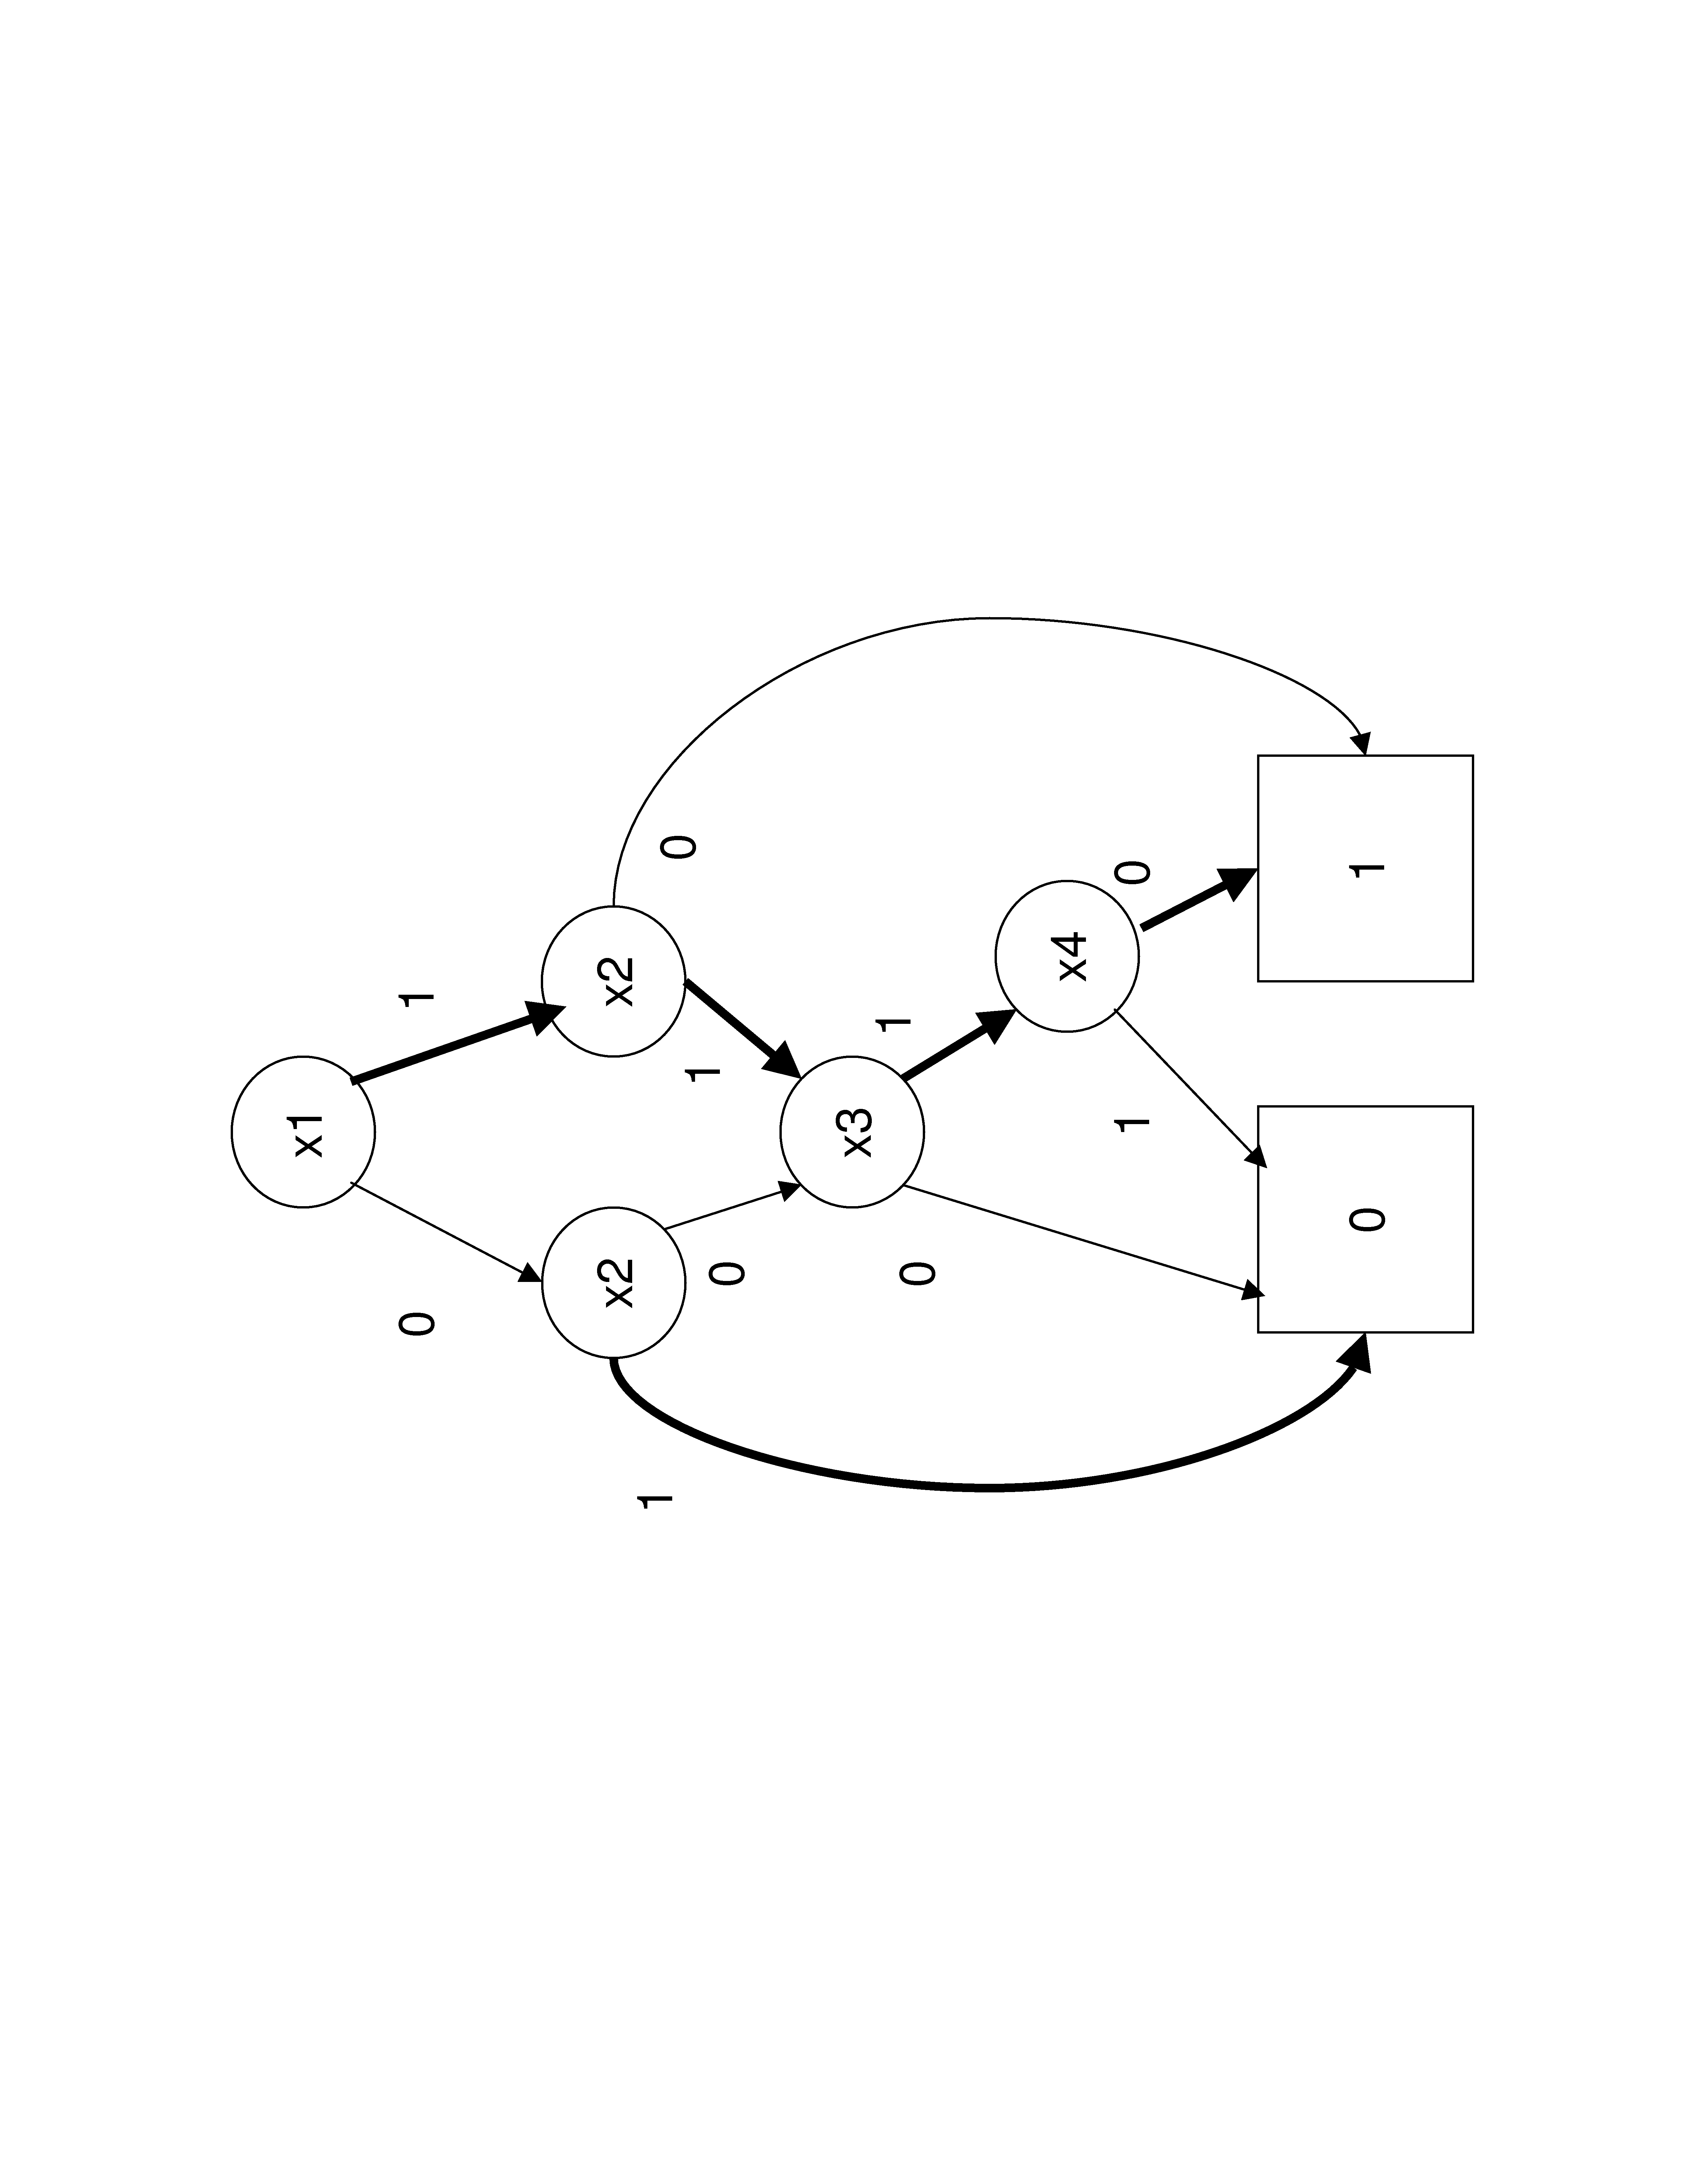
\includegraphics[scale=0.4,angle=270]{chapters/obdd1} 
\par\end{centering}

\caption{\label{fig:OBDD-example}OBDD for two-bit millionaires' problem}

\end{figure}


In \cite{kruger06}, we presented an SFE protocol that directly uses
an OBDD representation of the function $f$ to be jointly computed.
The advantage of using an OBDD representation over the Boolean gate-representation
is that OBDDs are more succinct for certain classes of functions than
the Boolean gate representation, including most linear functions.
For example, the OBDD representation is more efficient than the Boolean
gate representation for 8-bit AND, 8-bit addition, and the millionaires'
and billionaires' problems \cite{Yao86} OBDDs are not a universal
solution, however, for other functions, such as multiplication, the
OBDD can be far worse than the Boolean gate representation, due to
exponential node explosion \cite{Bryant:BDD}. For the classes of
functions in which the OBDD representation is efficient, our thesis
\cite{kruger06} shows that the protocol described next can perform
2 to 4 times better than the classical Yao protocol.

The protocol is loosely designed in a similar fashion as Yao's protocol
\cite{Yao86}. We present two variations of the protocol. An overview
of the 3 main steps of the protocols are shown in figure \ref{fig:OBDD-overview},
using the example millionaires' problem pictured above. In the first
step, Alice sends to Bob the encrypted OBDD. The next step is Bob
acquiring a subset of the encryption keys from Alice using $OT_{2}^{1}$.
In the final step, Bob uses the obtained keys to decrypt a single
path through the OBDD yielding the result of the computation. % A formal description follows. 


%
\begin{figure}
\begin{centering}
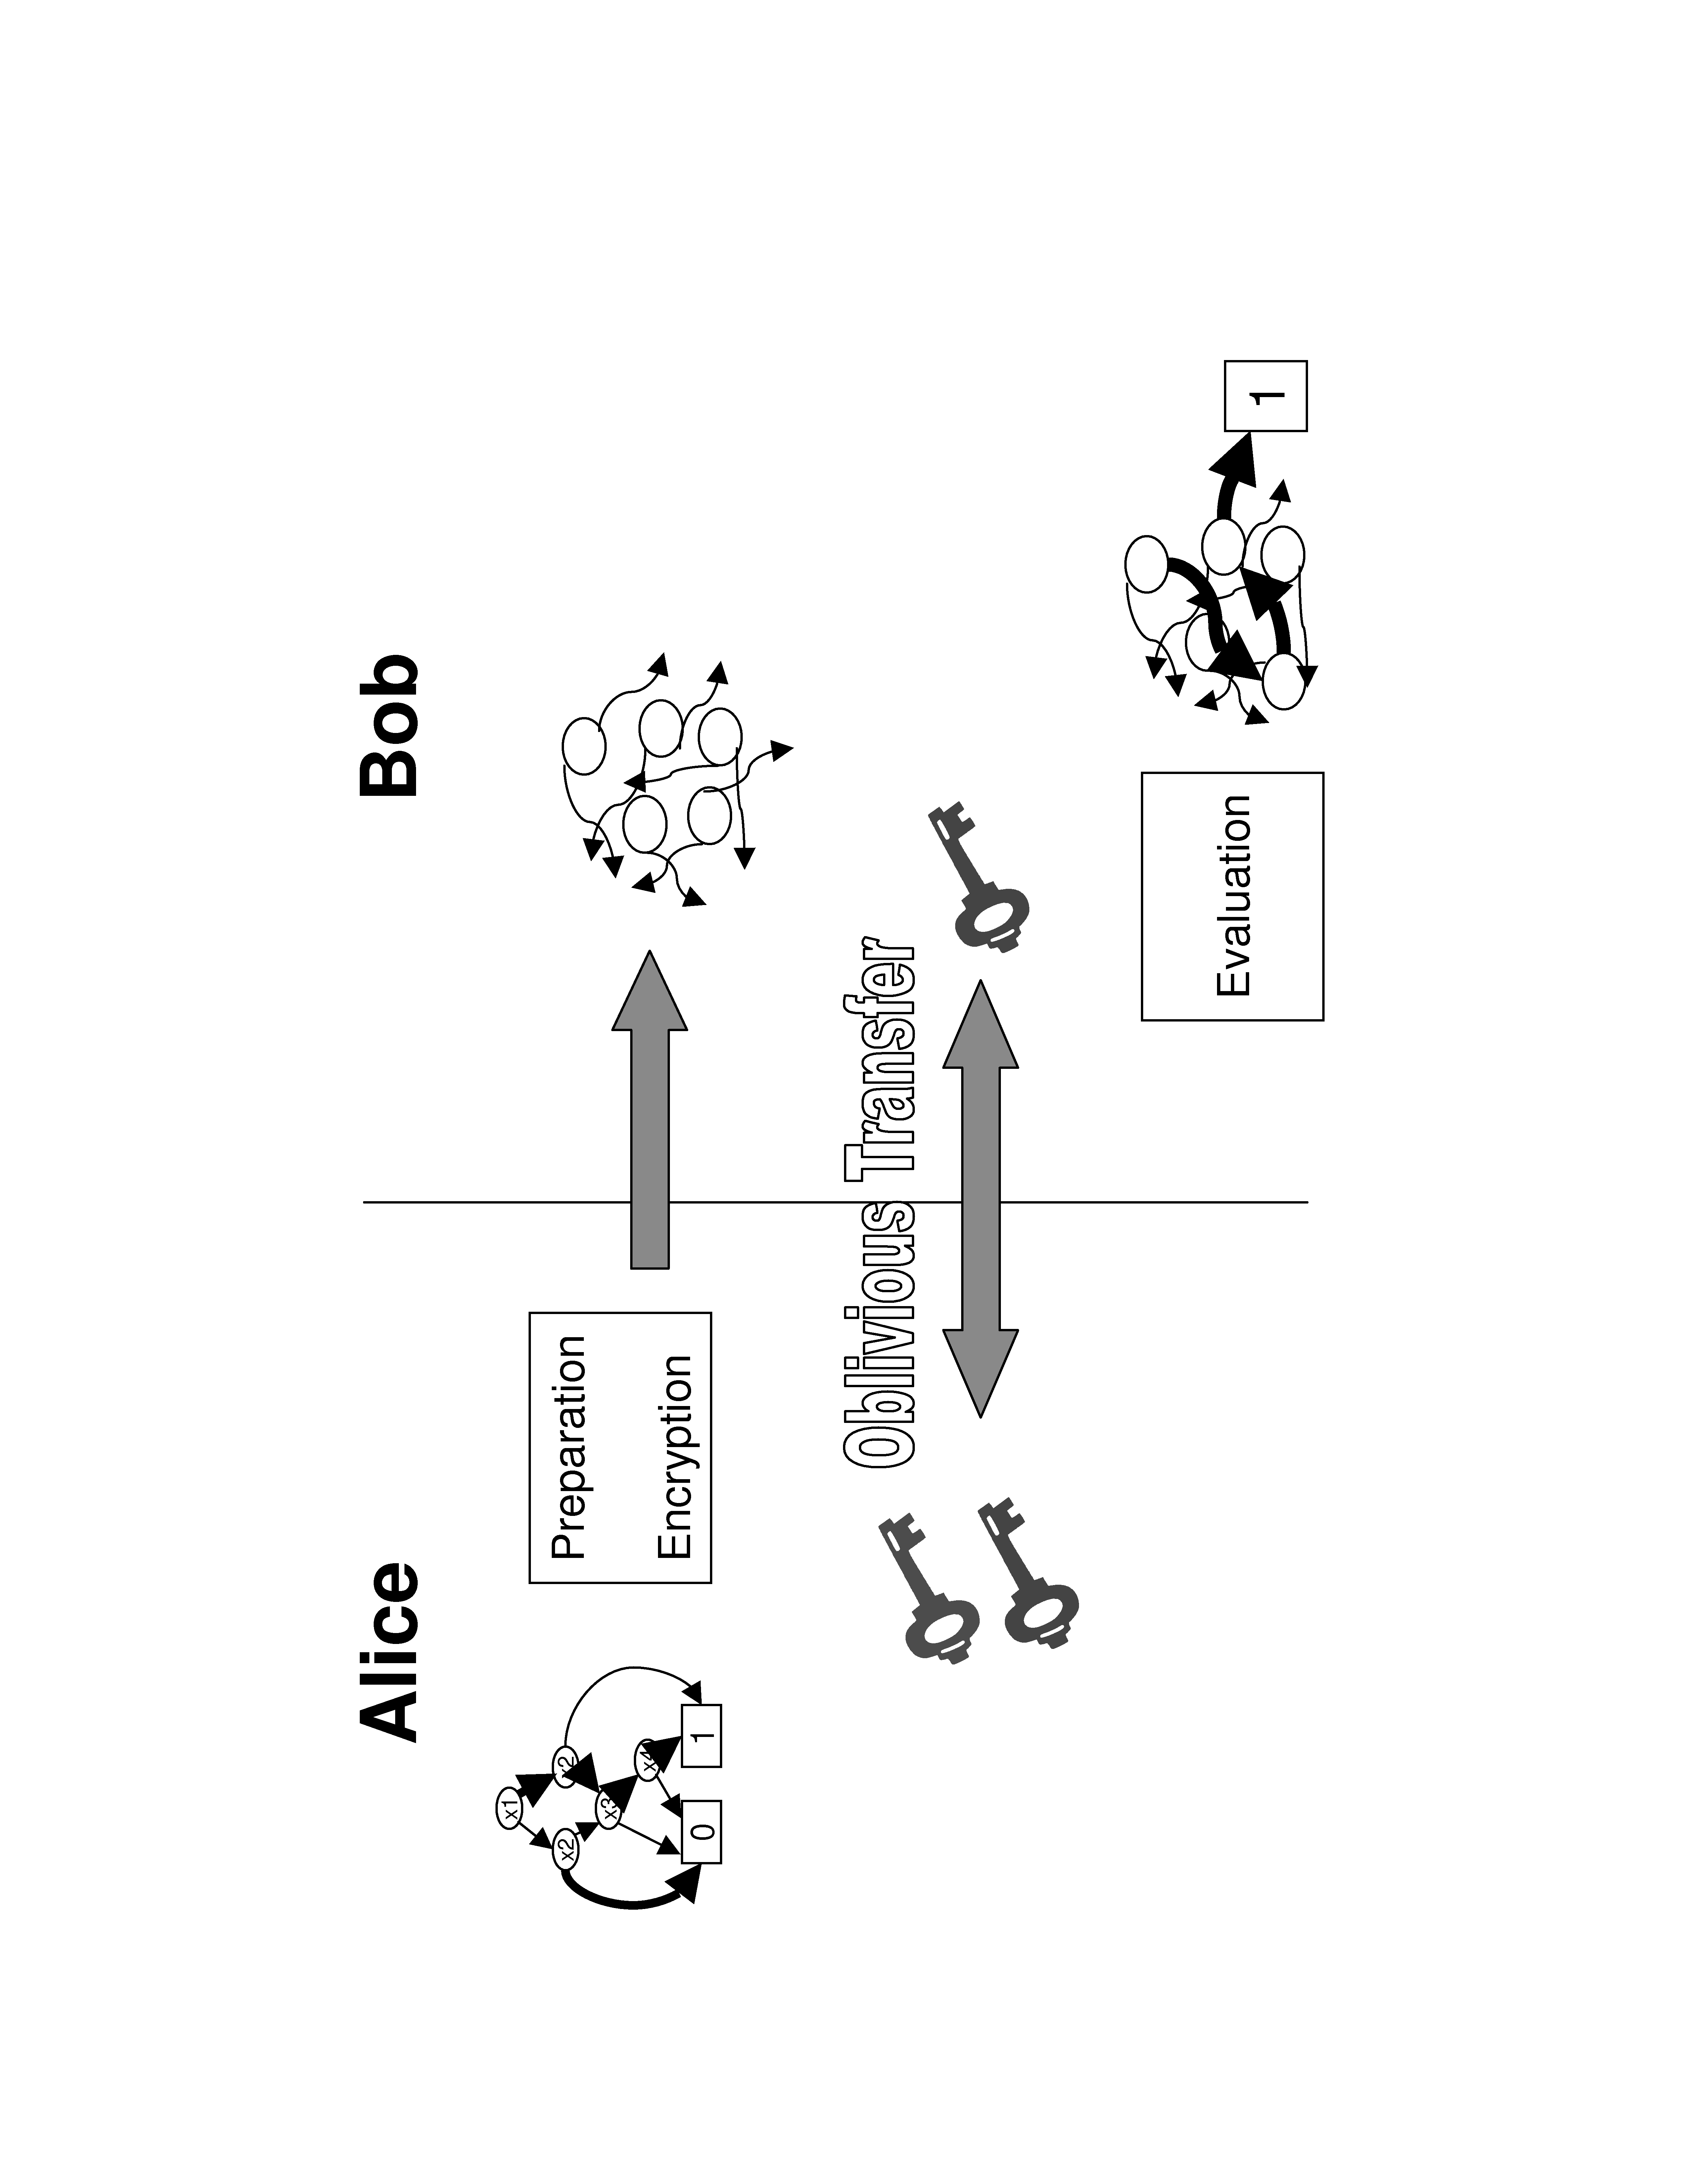
\includegraphics[scale=0.4,angle=270]{chapters/obdd_proto_overview} 
\par\end{centering}

\caption{\label{fig:OBDD-overview}OBDD secure evaluation protocol}

\end{figure}


%\begin{flushleft}
Assume that both parties' inputs include the $OBDD(f)$ for the Boolean
function $f(x_{1},x_{2},\cdots,x_{n})$ with the ordering $x_{1}<x_{2}<\cdots<x_{n}$.
Furthermore, Alice holds the inputs $(i_{1},\ldots,i_{k})$ corresponding
to the first $k$ variables $x_{1},\ldots,x_{k}$, and Bob has the
inputs $(i_{k+1},\ldots,i_{n})$.
\par\end{flushleft}
\begin{enumerate}
\item Alice performs the following steps: 

\begin{enumerate}
\item She traverses the $OBDD(f)$ using her input $(i_{1},\cdots,i_{k})$,
which results in a node $v_{init}$ at level $k$.
\item She uniformly and independently at random creates $(n-k)$ pairs of
secrets $(s_{1}^{0},s_{1}^{1}),\cdots,(s_{n-k}^{0},s_{n-k}^{1})$.
In addition, for each node $v$ in the $OBDD(f)$ whose level is between
$k$ and $n-1$, Alice also creates a secret $s_{v}$.
\item She assigns a uniformly random label to each node whose level is between
$k$ and $n$. We refer to the randomly assigned label of node $v$
using the notation $label(v)$.
\item Next, Alice augments $OBDD(f)$ with some number of dummy nodes (to
ensure that Bob always traverses $n-k$ nodes in his phase of the
protocol).
\item Alice garbles all nodes whose level is between $k$ and $n-1$ in
the following manner. Let $v$ be a node in $OBDD(f)$ such $k\leq{\it level}(v)\leq n-1$
and define ${\it level}(v)=\ell$. The encryption of node $v$, denoted
by $E^{(v)}$, is a label and a randomly ordered ciphertext pair \[
\left(label(v)\,\,,\,\, E_{s_{v}\oplus s_{\ell-k+1}^{0}}(label(low(v))\,\|\, s_{{\it low}(v)})\,\,\,,\,\,\, E_{s_{v}\oplus s_{\ell-k+1}^{1}}(label(high(v))\,\|\, s_{{\it high}(v)})\right)\,\,\,,\]
 where the labels are pre-pended to the secret with a separator symbol
and the order of the ciphertexts is determined by a fair coin flip.
Roughly speaking, the secrets corresponding to the $0$-successor
and $1$-successor of node $v$ are encrypted with the secret corresponding
to $v$ and its level.


Note that dummy nodes have the same structure as normal nodes, except
that the ciphertext pair contain encryptions of the same message since
dummy nodes have the same $0$ and $1$-successors. Provided the encryption
scheme is semantically secure, this poses no problem since the keys
are chosen uniformly at random.

Lastly, there are two terminal nodes of the form $(b,label(t_{b}))$
for $b=0$ or $1$. Recall that $OBDD(f)$ has two terminal nodes,
denoted as $0$ and $1$, that are at level $n$.

\item Once Alice is done encrypting, she sends to Bob the encryption of
all nodes whose level is between $k$ and $n$ and the secret $s_{v_{init}}$
corresponding to node $v_{init}$ at level $k$. We called this the
garbled OBDD.
\end{enumerate}
\item Bob performs the following steps: 

\begin{enumerate}
\item He engages in $n-k$ 1-out-of-2 oblivious transfers to obtain the
secrets corresponding to his input. For example, if his input $i_{j}$
is $0$, then he obtains the (level) secret $s_{j-k}^{0}$; otherwise,
he obtains the secret $s_{j-k}^{1}$.
\item Now Bob is ready to start his computation. Suppose $i_{k+1}=0$. With
$s_{1}^{0}$ and $s_{v_{init}}$, he decrypts both ciphertexts in
$E^{(v_{init})}$ and decides which gives the correct result by using
the verifiable range property of the encryption scheme. Bob now has
both $s_{{\it low}(v)}$ (the secret corresponding to the $0$-successor
of $v_{init}$) and $label(low(v))$ (which tells Bob which encrypted
node is used to evaluate his next input). Continuing this way, Bob
eventually obtains a label corresponding to one of the terminal nodes,
which determines the result of the OBDD on the shared inputs. Bob
sends this result to Alice. 
\end{enumerate}
\end{enumerate}




We then define an optimized variation which is identical to the protocol
just described, except that Alice first reduces the number of nodes
to be sent to Bob using an operation called \emph{restriction}, which
is a partial evaluation applied to OBDDs. Restriction is defined as
follows.

Given an $n$ variable Boolean function $f(x_{1},x_{2},\cdots,x_{n})$
and a Boolean value $b$, the restriction $f\mid_{x_{i}\leftarrow b}$
is a Boolean function of $n-1$ variables $x_{1},\cdots,x_{i-1},x_{i+1},\cdots,x_{n}$.
$f\mid_{x_{i}\leftarrow b}(x_{1},\cdots,x_{i-1},x_{i+1},\cdots,x_{n})$
is equal to $f(x_{1},\cdots,x_{i-1},b,x_{i+1},\cdots,x_{n})$. Essentially,
$f\mid_{x_{i}\leftarrow b}$ is the function obtained by substituting
the value $b$ for the variable $x_{i}$ in the function $f$. The
restriction operation can be performed over multiple variables by
restricting each variable independently, e.g., $f\mid_{x_{i}\leftarrow b,x_{j}\leftarrow b'}=(f\mid_{x_{i}\leftarrow b})\mid_{x_{j}\leftarrow b'}$.
The order in which the variables are restricted is unimportant.

\begin{flushleft}
For protocol 2, both parties' inputs include the $OBDD(f)$ for the
Boolean function $f(x_{1},x_{2},\cdots,x_{n})$ with the ordering
$x_{1}<x_{2}<\cdots<x_{n}$. Furthermore, Alice holds the inputs for
the variables in the set $X_{A}$ and Bob holds the inputs for the
variables in the set $X_{B}\;=\;\{x_{1},\cdots,x_{n}\}-X_{A}$. 
\par\end{flushleft}
\begin{enumerate}
\item Alice performs the following steps:

\begin{enumerate}
\item Alice computes the OBDD ${\cal O}_{A}$ as the restriction of her
inputs on the function $f\mid_{X_{A}}$. 
\item Alice encrypts the $O_{A}$ and sends it to Bob. This step is exactly
the same as in for Protocol 1. Alice also sends the secret corresponding
to the root of the OBDD ${\cal O}_{A}$. 
\end{enumerate}
\item The computation for Bob is exactly the same as that for Protocol 1. 
\end{enumerate}
The results of this work demonstrate that OBDDs showed improved performance
with secure evaluation of certain functions, as will be discussed
in chapter \ref{chapter:obdd}.

%\begin{comment}
\section{Problem Specific: Protocol Optimization of Evaluating Hash Functions
for Password Authentication}

In chapter \ref{chapter:pw}, based on our paper Secure Password Authentication
Using SFE \cite{Kruger10}, we use some properties of the problem
of authentication to transform the semi-honest protocol into an efficient
protocol that is secure in the malicious model. This work presents
a new solution to the {}``Secure Password and Key Authentication''
(SPAKA) problem, which is the design of protocols to mutually authenticate
a client to a server using 
\begin{enumerate}
\item The client's knowledge of the password X, and 
\item The servers's knowledge of a one-way hash function h(X). 
\end{enumerate}
The protocol must not leak any additional information or allow access
if one of the parties is an inposter and does not know their expected
credential. Our solution provides a property, unique among SPAKA protocols,
that it can work with arbitrary and legacy hash functions used in
commodity operating systems today. This protocol takes advantage of
specific properties of the authentication problem and takes {}``shortcuts''
to achieve efficiency. Although these shortcuts would not be secure
in a general SFE setting, we prove that these shortcuts are in fact
secure in the context of the authentication protocol presented. This
allows us to design a protocol in which a malicious adversary is thwarted
with probability $1-2^{-l}$ where $l$ is a security parameter representing
the number of semi-honest circuits. We show that on modern multicore
processors, the authentication can be performed in a matter of seconds,
which we believe is practical for interactive use between servers
and authenticating users.
%\end{comment}

\section{Class of Algorithm Specific: Protocol Optimization of Dynamic Programming}

In this work, presented in detail in chapter \ref{chapter:genomics},
we considered a design \emph{methodology} for creating secure protocols
based on typical dynamic programming algorithms. Unlike the OBDD protocol
discussed in the previous section, this is not an automatic tool for
generating secure protocols, but rather a set of concepts that are
applicable to designing secure protocols for evaluating dynamic programming
algorithms. We illustrate these ideas with several example protocols
for computing the edit distance problem, which is the minimum number
of character insertions, deletions, and substitutions needed to change
string $x$ to string $y$.

Let ${\cal P}(x,y)$ be a problem with two inputs $x$ and $y$. Typically,
a dynamic-programming algorithm ${\cal A}_{{\cal P}}$ for problem
${\cal P}$ has the following components: 
\begin{itemize}
\item A set $S$ of sub-problems and a dependency relation $R\subseteq S\times S$
between the sub-problems. Intuitively, $(s,s')\in R$ means that the
sub-problem $s'$ depends on the sub-problem $s$. If there is a dependency
between $s$ and $s'$, we write it as $s\rightarrow s'$. In the
case of the problem of computing edit-distance between two strings
$\alpha$ and $\beta$ of length $n$ and $m$, the set of sub-problems
is $[0,\cdots,n]\times[0,\cdots,m]$. For all sub-problems $(i,j)$
such that $i\not=0$ and $j\not=0$, we have the following dependencies:
$(i-1,j)\rightarrow(i,j)$, $(i,j-1)\rightarrow(i,j)$, and $(i-1,j-1)\rightarrow(i,j)$.
The \textit{base sub-problems} are $s\in S$ such that they have no
dependencies. For the edit-distance problem, the base sub-problems
are: \[
\begin{array}{l}
\{(i,0)\;\mid\;0\leq i\leq n\}\\
\{(0,j)\;\mid\;0\leq j\leq m\}\end{array}\]
 We also assume that there is a unique root sub-problem ${\it root}\in S$
such that there does not exist a sub-problem that depends on ${\it root}$.
For the edit-distance problem the unique root sub-problem is $(n,m)$. 
\item Each sub-problem $s$ is assigned a value ${\it val}(s)$. The goal
is to compute ${\it val}({\it root})$. The function ${\it val}$
from $S$ to $\Re$ assigns values to sub-problems, such that it satisfies
the following properties:

\begin{itemize}
\item For all the base sub-problems $s\in S$, ${\it val}(s)$ is defined. 
\item Let $s\in S$ be a non-base sub-problem. Define ${\it pred}(s)$ as
all the predecessors of $s$, i.e. the set ${\it pred}(s)$ is defined
as $\{s'\;\mid\; s'\rightarrow s\}$. Assume that ${\it pred}(s)$
is equal to $\{s_{1},\cdots,s_{k}\}$. There is a recursive function
$f$ defining ${\it val}(s)$ in terms of ${\it val}(s_{1}),{\it val}(s_{2}),\cdots,{\it val}(s_{k})$,
$s(x)$, and $s(y)$, where $s(x)$ and $s(y)$ are parts of the input
$x$ and $y$ that are relevant to the sub-problem $s$. In case of
the edit-distance problem ${\it val}((i,j))$ is equal to $D(i,j)$. 
\end{itemize}
\end{itemize}
We implemented three variations of the protocol in \cite{kruger07},
and showed that the techniques produce efficient ways to compute the
edit distance of two strings. For example, the protocol is able to
compute the edit distance of two strings of length $200$ (which has
$200^{2}=40000$ sub-computations), in under 10 minutes. Our most
efficient protocol computes elements of the dynamic programming matrix
in large blocks during each round of the computation. We experimentally
determined than a block size of $(20,20)$ yielded an optimum trade-off
between a decreased number of rounds, and larger block circuits. Using
a $(20,20)$ circuit allows $20^{2}=400$ elements of the matrix to
be evaluated during each round of the protocol, which allows the overall
$(200,200)$ problem to be evaluated in $100$ rounds. In comparison,
using the generic techniques to compile the edit distance algorithms
into a secure circuit produced circuits which were to too large for
evaluation beyond problems of size $(25,25)$.


\section{Algorithm Specific: Protocol Optimization of K-Means Clustering}

The $k$-means algorithm is a common clustering technique in data
mining. Suppose that we are given $n$ samples $x_{1},\cdots,x_{n}$,
where each sample is a $m$-dimensional vector of real numbers. The
problem is to assign the samples to $c$ clusters in such a manner
that similar points are grouped together. Similarity is defined using
a distance metric. The standard clustering algorithm maintains $c$
means $\mu_{1},\cdots,\mu_{c}$. Initially, assume that the means
are assigned arbitrary values. A sample $x_{i}$ is deemed to be in
the cluster $j$ if it is closest to the mean $\mu_{j}$, where mean
of a cluster $\{x'_{1},\cdots,x'_{r}\}$ is $\frac{x'_{1}+\cdots,x'_{r}}{r}$.
In a Euclidean space, the distance between two $m$-dimensional vectors
$x$ and $y$ is $\sum_{j=1}^{m}(x[j]-y[j])^{2}$, where $x[j]$ is
the $j$-th element of the vector $x$. Other distance metrics~\cite[Chapter 10]{pattern-classification},
such as scatter metrics, can be used instead of the distance metric
mentioned above. Each iteration of the $k$-means algorithms recomputes
the means and reclassifies the samples. The algorithm terminates when
it detects no change in the means. See \ref{fig:clusters} for an
illustration.

%
\begin{figure}
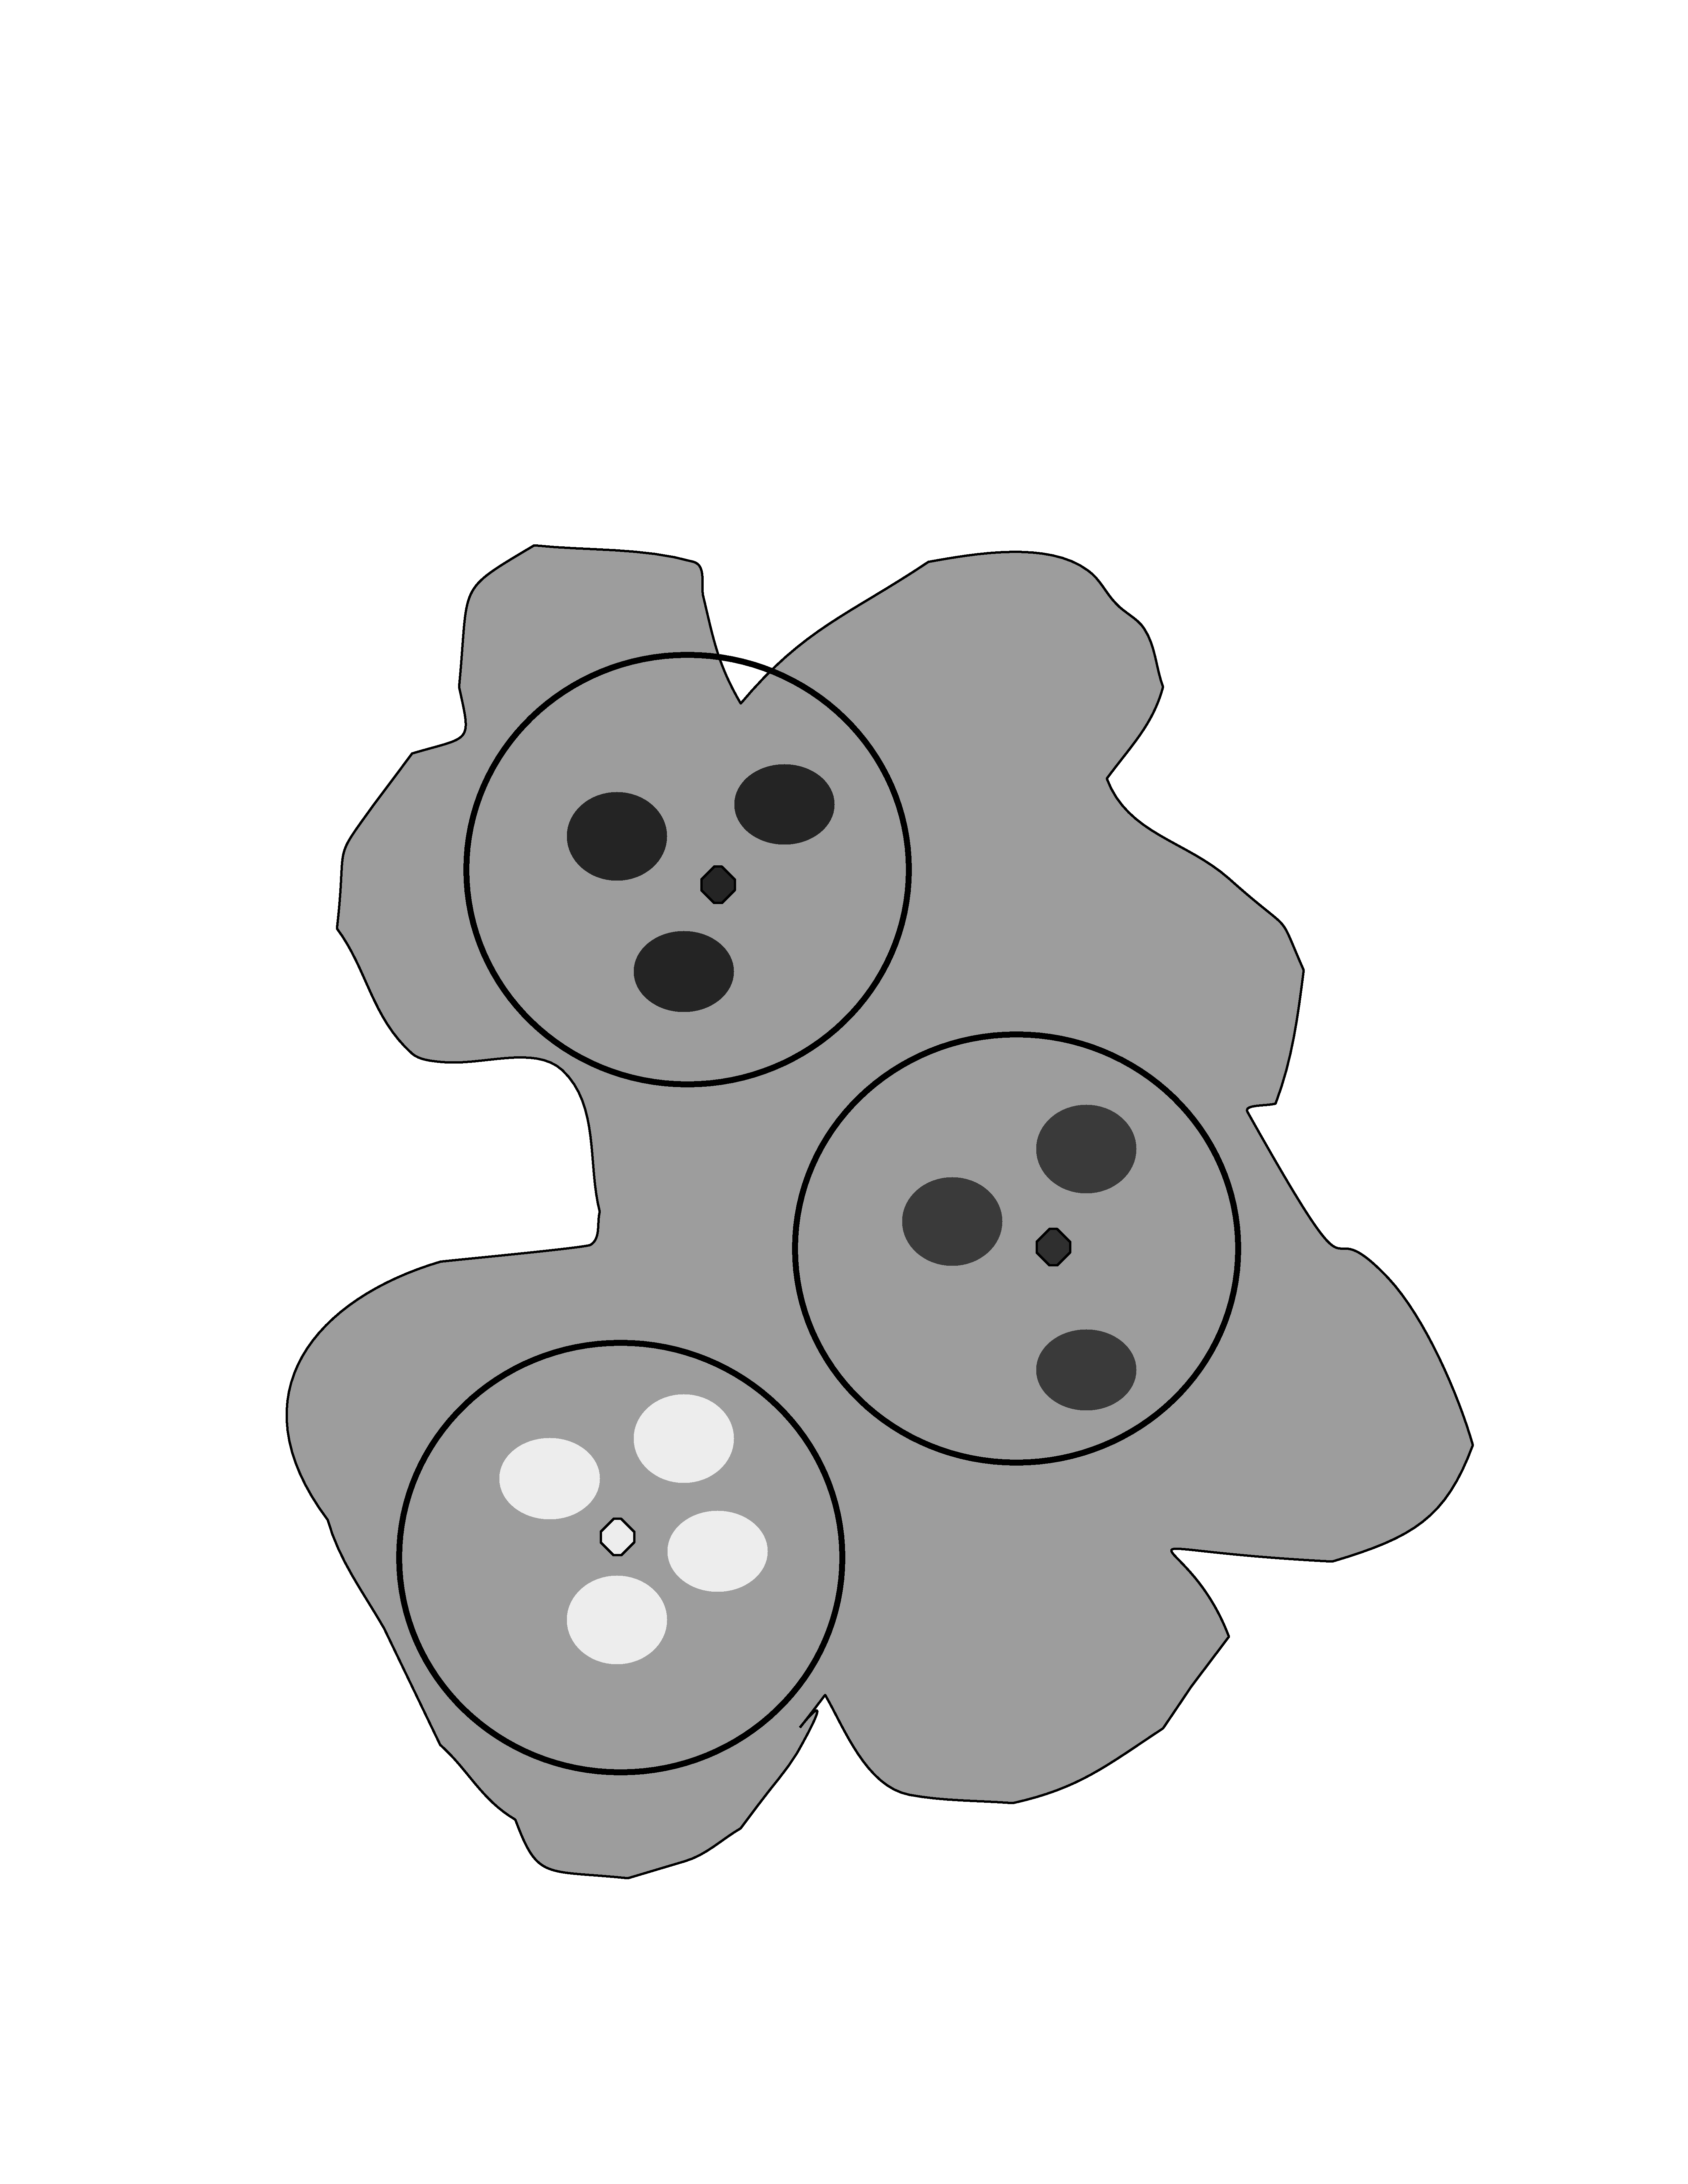
\includegraphics[scale=0.3,angle=270]{chapters/clusters}

\caption{\label{fig:clusters}Thirteen data points after clustering. The small
dots are cluster means.}

\end{figure}


We implement protocols to securely evaluate this algorithm in chapter
\ref{chapter:kmeans} based on our paper \cite{kruger05}, and showed
that a protocol based on homomorphic encryption was able to classify
partitioned data sets with tens of thousands of data points in under
two minutes, which is about 15 times slower than the protocol implemented
without privacy protection, and over 100 times faster than the same
protocol built with Yao circuits.


\section{Other Optimizations}

\label{sub:Other-Optimizations}

In the usual formulation of secure function evaluation, there are
designated outputs for each party, and it is required that no extra
information is learned by any party. This definition could be expanded
to assign non-output values the labels {}``sensitive'' and {}``non-sensitive'',
where the protocol is considered secure if no sensitive information
is leaked. %Since the overhead of privacy protection is substantial,
%I propose to research the of design secure protocols that use this
%relaxation of the problem definition to improve efficiency. 


In section \ref{sub:Primitives}, I presented many basic cryptographic
primitives that are used in SFE. Improving the state of the art of
any one of those primitives would automatically benefit all SFE protocols
that make use of that primitive. Based on my experience with real
implementations of SFE protocols, the oblivious transfer steps tend
to be very expensive in terms of space and communication. Common oblivious
transfer protocols are based on discrete logarithms, but other trapdoor
functions may be used as well. %One thing I propose to try is implementing
%Naor-Pinkas \cite{Noar-Pinkas:2001} using more compact representations,
%for example, with elliptic curve groups. I have recently developed
A new $OT_{2}^{1}$ protocol is presented in chapter \ref{sec:OT-SquareRoots}.
and its security and performance are compared with the Naor-Pinkas
protocol. %In particular, I conjecture that this protocol
%may require less communication overhead than other OT protocols.


%
\begin{comment}

\chapter{An Efficient Protocol Design Framework}

\label{sub:An-Efficient-Framework}

Even with all these optimizations, protocols still must be hand-coded.
Each protocol I have implemented has required brand new code to be
written, with only some common cryptographic primitives being shared
between implementations. In this case, I define the term protocol
to mean a structured sequence of communications between parties which
enables the computation to performed. Fairplay \cite{Fairplay} suggested
the idea of having a common framework for protocol design, but because
Fairplay is a straightforward implementation of Yao's garbled circuit
method \cite{Yao86}, it suffers from poor performance. Fairplay's
contribution is to create a compiler for expressing algorithms functionally,
and compiling them into a circuit representation suitable for secure
evaluation. In this sense, it functions as a simple CAD design tool.

I propose to take this concept much further, and create an \emph{optimizing}
protocol compiler, aggregating the techniques discussed here, and
creating a tool to greatly simplify the creation of efficient secure
protocols for SFE. The compiler will include the following components: 
\begin{itemize}
\item Convenient programming language for expressing secure computations

\begin{itemize}
\item Language will include support as language primitives for common SFE
and cryptographic techniques, such as homomorphic encryption 
\item Language will support metadata for designating inputs and outputs
from specific parties, and for classifying the required privacy of
intermediate computations 
\end{itemize}
\item Compiler which translates this language into an abstract securely
evaluable {}``machine code'', which consists of securely evaluable
representations of the program. 
\item An automated optimizer. The optimizer will automatically try different
representations of the functions, including OBDDs, Boolean circuits,
and other ideas from my research, and search for the most efficient
representation as possible. 
\item Manual optimization tools, making it convenient to apply and design
techniques that I have researched. This includes a toolkit of cryptographic
protocols, such as oblivious transfer, which can be used in a black
box way. 
\item An embeddable protocol evaluator library, which will allow ordinary
application to make straightforward use of secure function evaluation. 
\end{itemize}
The security of protocols produced by the compiler is based on the
security of each individual component of the protocol. For example,
when choosing optimal circuit representations, the compiler will choose
among several possible representations, each of which has a corresponding
secure evaluation protocol. In cases where a computation is broken
into multiple sub-protocols, I will prove that composition of these
sub-protocols maintains the overall security of the protocol.

\bibliographystyle{plain} \bibliographystyle{plain}
\bibliography{somesh}

\end{comment}
{} 

%\chapter{Privacy Preserving Genomics}
\chapter{Practical Privacy for Genomic Computation}

%Secure function evaluation is practical.

\section{Contribution}
\label{sec:obdd-intro}

% Importance of Privacy has spurred interest in privacy-preserving
% protocols.

% Mention importance of BDDs and their applications.
% Describe that it is graph-based data structure.
% Describe our basic contribution.

{\it Ordered Binary Decision Diagrams (OBDDS)}, introduced and
described in section 3.?, are a graph-based representation of Boolean
functions.  We present an
SFE algorithm that directly uses an OBDD representation of the
function $f$ that the two parties want to jointly compute. 

% List of contributions.
Our thesis presents the following contributions:
\begin{itemize}
\item We present a SFE protocol that uses the OBDD representation of
the function to be jointly computed by two parties. Our new protocol along with the
correctness proof is provided in Section~\ref{sec:sfe-obdd}.

\item 
Experimental results based upon a prototype implementation of our
protocol demonstrate that for certain functions, our
implementation results in a smaller encrypted circuit than
the equivalent Yao circuit. For example, for the classic millionaire's problem, our
implementation reduces the bandwidth by approximately $45$\% over the Yao
protocol.  Our
implementation and experimental results are described in
Section~\ref{sec:experiments}.
\end{itemize}

The
advantage of using an OBDD representation over the gate-representation
is that OBDDs are more succinct for certain widely used classes of
functions than the gate representation. For example, among other
functions, our results show the OBDD representation is more efficient
than the gate representation for 8-bit AND, 8-bit addition, and the
millionaire's and billionaire's problems~\cite{Yao:86}.  As a result,
our protocol has reduced bandwidth consumption over the classic Yao
protocol.  Because processor speeds have
increased at a more rapid pace than bandwidth availability over the
past years, network bandwidth is likely to be the bottleneck for a number of applications. In particular, our
protocols are especially useful for applications operating over
networks with limited bandwidth, such as wireless and sensor networks.
Furthermore, we have empirically confirmed this statement by
implementing our protocol and comparing it with the Yao protocol.

In summary, our thesis presents a new SFE protocol that uses the OBDD representation.
The OBDD representation is more efficient for several practical functions of 
interest. For other functions, the circuit description (and therefore
FairPlay) will be more efficient. This protocol presents a generic alternative to 
Boolean circuits that can be used when appropriate. 



\section{Cryptographic Toolkit}
\label{crypto}

We will employ several standard cryptographic techniques.

\vspace{1ex}
\noindent
\textbf{Oblivious transfer.}
\emph{Oblivious transfer} was originally proposed by Rabin~\cite{R81}.
Informally, a $1$-out-of-$n$ oblivious transfer (denoted as $OT_1^n$)
is a protocol between two parties, the chooser and the sender.
The sender's inputs into the protocol are $n$ values $v_1,\ldots,v_n$.
The chooser's input is an index $i$ such that $1 \leq i \leq n$.
As a result of the protocol, the chooser receives $v_i$, but does not
learn anything about the rest of the sender's values.  The sender learns
nothing.  Our protocols do not depend on a particular implementation of
oblivious transfer; therefore, we simply assume that we have access to a
cryptographic primitive implementing $OT_1^2$.  In our implementations,
we rely on Fairplay~\cite{Fairplay} and the Naor-Pinkas oblivious transfer
construction~\cite{Naor-Pinkas:2001}.

\vspace{1ex}
\noindent
\textbf{Oblivious circuit evaluation.}
\label{yao}
We also employ two standard methods for secure circuit evaluation: Yao's
``garbled circuits'' method and secure computation with shares.  Consider
any (arithmetic or Boolean) circuit $C$, and two parties, Alice and Bob,
who wish to evaluate $C$ on their respective inputs $x$ and $y$.  

Yao's ``garbled circuits'' method was originally proposed in~\cite{Yao86}
(a complete description and security proofs can be found in~\cite{LP04}).
Informally, Alice securely transforms the circuit so that Bob can
evaluate it without learning her inputs or the values on any internal
circuit wire except the output wires.

Alice does this by generating two random keys for each circuit wire,
one representing $0$ on that wire, the other representing $1$.  The keys
representing Alice's own inputs into the circuit she simply sends to
Bob.  The keys representing Bob's inputs are transferred to Bob via the
$OT_1^2$ protocol.  For each of Bob's input wires, Bob acts as the chooser
using his input bit on that wire as his input into $OT_1^2$, and Alice
acts as the sender with the two wire keys for that wire as her inputs
into $OT_1^2$.  If Bob has a $q$-bit input into the circuit, then $q$
instances of $OT_1^2$ are needed to transfer the wire keys representing
his input, since each input bit is represented by a separate key.

Alice produces the ``garbled'' truth table for each circuit gate in
such a way that Bob, if he knows the wire keys representing the values
on the gate input wires, can decrypt exactly one row of the garbled
truth table and obtain the key representing the value of the output wire.
For example, consider an AND gate whose input wires are $a$ and $b$,
and whose output wire is $c$.  Let $k^0_a,k^1_a,k^0_b,k^1_b,k^0_c,k^1_c$
be the random wire keys representing the bit values on these wires.
The garbled truth table for the gate is a random permutation of
the following four ciphertexts:
$E_{k^1_a}(E_{k^0_b}(k^0_c))$,
$E_{k^1_a}(E_{k^1_b}(k^1_c))$.
$E_{k^0_a}(E_{k^1_b}(k^0_c))$,
$E_{k^0_a}(E_{k^0_b}(k^0_c))$.
Yao's protocol maintains the invariant that for every circuit wire,
Bob learns \emph{exactly one} wire key.

Because wire keys are random and the mapping from wire keys to values
is not known to Bob (except for the wire keys corresponding to his own
inputs), this does not leak any information about actual wire values.
The circuit can thus be evaluated ``obliviously.''  For example, given
the above table and the input wire keys $k^0_a$ and $k^1_b$ representing,
respectively, $0$ on input wire $a$, and $1$ on input wire $b$, Bob
can decrypt exactly one row of the table, and learn random key $k^0_c$
representing $0$ (\ie, the correct result of evaluating the gate) on
the output wire $c$.

Observe that until Alice reveals the mapping, Bob does \emph{not}
know which bits are represented by the wire keys he holds.  For the
standard garbled circuit evaluation, Alice reveals the mapping only
for the wires that represent the output of the entire circuit, but
not for the intermediate wires.

Several of our protocols rely on the representation of bit values on
circuit wires by random keys.   These protocols use Yao's construction
not as a ``black box'' implementation of secure circuit evaluation,
but exploit its internal structure in a fundamental way.

The second standard method is \emph{secure computation with shares}
(SCWS)~\cite[Chapter 7]{Goldreich:vol2}.  This protocol maintains
the invariant that, for every circuit wire $w$, Alice learns a random
value $s$ and Bob learns $b_w - s$, where $b_w$ is the bit value of
the wire.  Therefore, Alice's and Bob's shares add up to $b_w$, but
because the shares are random, neither party knows the actual wire value.
For each output wire of the circuit, Alice and Bob combine their shares to
reconstruct the circuit output.  

% Either Yao's ``garbled circuits'' method,
% or SCWS can be used to securely and privately evaluate any circuit $C$.


\section{Privacy-Preserving Protocol for \\ the Weighted Average Problem}
\label{sec:WAP}

In the weighted average problem (WAP) we want to find
a privacy-preserving protocol for the following functionality:
\begin{eqnarray*}
((x,n),(y,m)) & \longmapsto & (\frac{x+y}{n+m}, \frac{x+y}{n+m})
\end{eqnarray*}
Recall that a protocol for WAP was used in
the privacy-preserving $k$-means algorithm (see Figure~\ref{fig:pp-k-means}).


A simple strategy to address this problem is to first approximate the
function $\frac{x+y}{n+m}$ by a circuit $C$, and then use standard
constructions~\cite{Goldreich87,Goldreich:JACM:91,Yao86} to construct
a privacy-preserving protocol.  Protocols constructed using this
strategy have a very high computational overhead. Malkhi {\it et al.} 
considered the cost of implementing these protocols in their work in
the Fairplay system~\cite{mnps04}.  They found that the protocol was
feasible for small circuits, e.g., a single $\wedge$-gate could be
implemented in $410$ milliseconds, and more complex integer numerical
functions could be implemented on the order of seconds.  They further
showed the runtimes of these protocols grow quickly with the size of
the input and complexity of the implemented function.  The most
complex function discussed by the authors computed a median of two
ten-element integer input sets.  This function took over $7$ seconds
to execute in a LAN environment, and over $16$ seconds in an WAN
environment.  The circuit for computing $\frac{x+y}{n+m}$ is
significantly more complex. Hence, with a non-trivial data set, a
single computation of cluster means may take several minutes to compute.  Note that
the underlying costs of Fairplay are not artifacts of the design, but
simply the cost of implementing the standard protocols; the reported
costs were almost completely dominated with circuit setup and the
necessary oblivious transfers.

In this section, we present two privacy-preserving protocols for WAP
that are more efficient than the standard protocols. The first
protocol is based on oblivious polynomial evaluation and the second on
homomorphic encryption. Similarity of WAP with a problem that occurs
in protocols for generation of shared RSA
keys~\cite{Boneh-Franklin-2001,Gilboa99} is discussed in
appendix~\ref{sec:shared-RSA}.


\subsection{Protocol based on oblivious polynomial evaluation}
\label{subsec:OPE}

We will first give a privacy-preserving protocol for a general problem,
and then at the end of the subsection demonstrate how we can construct
a privacy-preserving protocol for WAP.  Consider the following
problem.

\begin{definition}
\rm
Let ${\cal F}$ be a finite field. Party $1$ has two polynomials $P$
and $Q$ with coefficients in ${\cal F}$. Party $2$ has two points
$\alpha$ and $\beta$ in ${\cal F}$. Both parties want to compute
$\frac{P(\alpha)}{Q(\beta)}$. In other words, we want to privately
compute the following functionality:
\begin{eqnarray*}
((P,Q),(\alpha,\beta)) & \longmapsto & (\frac{P(\alpha)}{Q(\beta)},\frac{P(\alpha)}{Q(\beta)})
\end{eqnarray*}
We call this problem {\em private rational polynomial evaluation (PRPE)}.
\end{definition}

The protocol $\mathcal{P}_{PRPE}$
uses a protocol for oblivious polynomial evaluation, which is defined below.

\begin{definition}
\rm
Let $\mathcal{F}$ be a finite field.  The {\em oblivious polynomial
evaluation} or {\em OPE} problem can be defined as follows: Alice
$A$ has a polynomial $P$ over the finite field $\mathcal{F}$, and
Bob $B$ has an element $x \in \mathcal{F}$. After executing the  protocol
implementing OPE $B$ should {\em only know} $P(x)$ and $A$ should
know nothing.
\end{definition}

A protocol to solve the OPE was  given by Naor and
Pinkas~\cite{NaorPinkas99}.  Let $\mathcal{P}_{OPE}(P,\alpha)$ denote
the privacy-preserving protocol for OPE. We provide a protocol
$\mathcal{P}_{PRPE}((P,Q),(\alpha,\beta))$ for PRPE, which uses
$\mathcal{P}_{OPE}(P,\alpha)$ as an oracle. The protocol is shown in
Figure~\ref{fig:PRPE}. 

\begin{figure}
\framebox{\parbox[c]{6.5in}{
{\bf (Step 1)} Party $1$ picks a random element $z \in \mathcal{F}$ and
computes two new polynomials $zP$ and $zQ$. In other words,
party $1$ ``blinds'' the polynomials $P$ and $Q$.
\medskip\\
{\bf (Step 2)} Party $2$ computes $z P(\alpha)$ and $z Q(\alpha)$ by
invoking the protocol for OPE twice, i.e., invokes the 
protocol $\mathcal{P}_{OPE}(zP,\alpha)$ and $\mathcal{P}_{OPE}(zQ,\beta)$.
\medskip\\
{\bf (Step 3)} Party $2$ computes $\frac{P(\alpha)}{Q(\beta)}$ by computing
$\frac{z P(\alpha)}{z Q(\beta)}$ and sends it to party $1$.
}}
\caption{Protocol for PRPE.}
\label{fig:PRPE}
\end{figure}


\begin{theorem}
\rm
\label{thm:privacy-PRPE}
Protocol $\mathcal{P}_{PRPE}((P,Q)(\alpha,\beta)$ shown in Figure~\ref{fig:PRPE}
is privacy-preserving protocol for PRPE.
\end{theorem}
{\bf Proof:} The views of the two parties are
\begin{eqnarray*}
\mbox{VIEW}_1^{\mathcal{P}_{PRPE}} (P,Q) & = & (P,Q,\frac{P(\alpha)}{Q(\beta)}) \\
\mbox{VIEW}_2^{\mathcal{P}_{PRPE}} (\alpha,\beta) & = & (\alpha,\beta, z P(\alpha), z Q(\beta))
\end{eqnarray*}
The view of party $1$ consists of its input $(P,Q)$ and output $\frac{P(\alpha)}{Q(\beta)}$.
Therefore, there is nothing to prove (see definition~\ref{def:privacy}, we can use
$S_1$ as the identity function). The input and
output of party $2$ are $(\alpha,\beta)$ and $\frac{P(\alpha)}{Q(\beta)}$ respectively.
We have to show a PPTA $S_2$ such that
$S_2 (\alpha,\beta,\frac{P(\alpha)}{Q(\beta)})$ and $\mbox{VIEW}_2^{\mathcal{P}_{PRPE}} (\alpha,\beta)$
are statistically indistinguishable. Let $z'$ be a random element of $\mathcal{F}$ and $S_2 (\alpha,\beta,\frac{P(\alpha)}{Q(\beta)})$
be defined as follows:
\[
(\alpha,\beta, z' \frac{P(\alpha)}{Q(\beta)},z')
\]
It is easy to see that the following two ensembles are statistically indistinguishable:
\[
\begin{array}{l}
(\alpha,\beta, z' \frac{P(\alpha)}{Q(\beta)},z') \\
(\alpha,\beta, z P(\alpha), z Q(\beta))
\end{array}
\]
The reason is that if $z$ is a random element of $\mathcal{F}$ then $z
Q(\beta)$ is a random element of $\mathcal{F}$ as well. Moreover, the
ratio of the third and fourth elements in the view of party $2$ is
$\frac{P(\alpha)}{Q (\beta)}$, i.e., the output and the third element
of the view determine the fourth element of the view.

Recall that $\mathcal{P}_{PRPE}$ uses the protocol $\mathcal{P}_{OPE}$.
Using the composition theorem we conclude that $\mathcal{P}_{PRPE}$ 
is privacy preserving.
$\Box$

\paragraph{Protocol for WAP.} First, we show that a protocol $\mathcal{P}_{PRPE}$ for PRPE can be
used to solve WAP. Recall that in WAP party $1$ and party $2$ have inputs
$(x,n)$ and $(y,m)$ respectively. In the invocation of $\mathcal{P}_{PRPE}$, party $1$
constructs two polynomials $P(w) = w + x$ and $Q(w) = w + n$, and party $2$
sets $\alpha = y$ and $\beta = m$. The output both parties receive is equal
to $\frac{x+y}{n+m}$, which is the desired output. The proof of privacy
for this protocol follows from Theorem~\ref{thm:privacy-PRPE} and the composition
theorem.


\subsection{Protocol based on homomorphic encryption}
\label{subsec:homomorphic}

Let $(G,E,D,M)$ be a encryption scheme (where $G$ is the function to
generate public parameters, $E$ and $D$ are the encryption and
decryption functions, and $M$ is the message space respectively) with
the following properties:
\begin{itemize}
\item The encryption scheme $(G,E,D)$ is {\em semantically secure}~\cite{Goldwasser:Micali}.
Essentially, an encryption scheme is semantically secure
if an adversary gains no extra information by inspecting the ciphertext.
This is formally defined in the appendix (see definition~\ref{def:semantic-secure}).


\item  For all $m \in M$ and $\alpha \in M$, $m_1 \in E(m)$
implies that $m_1^\alpha \in E(m \alpha)$. Encrypting the same
message twice in a probabilistic encryption function can
yield a different ciphertext, so $E(m)$ denotes the set of
ciphertexts that can be obtained by encrypting $m$.\footnote{
Of course, to successfully decrypt  two different messages
$m$ and $m'$ sets $E(m)$ and $E(m')$ should be disjoint.}

\item There is a computable function $f$ such that for all messages $m_1$ and $m_2$
the following property holds:
\begin{eqnarray*}
f(E(m_1),E(m_2)) & = & E (m_1+m_2)
\end{eqnarray*}
\end{itemize}
There are several encryption scheme that have the three properties
mentioned above~\cite{Benaloh:94,Naccache-Stern,Paillier99}. In our
implementation, we used the {\it dense probabilistic encryption (DPE)}
scheme of Benaloh~\cite{Benaloh:94}. The semantic security of the
scheme provided by Benaloh is based on the intractability of 
deciding prime residuosity.



Party $1$ and $2$
have a pair of messages $(x,n)$ and $(y,m)$. The two parties want to
jointly compute $\frac{x+y}{n+m}$ in a privacy-preserving way. Assume
that party $1$ sets up a probabilistic encryption scheme $(G,E,D,M)$, and
publishes the public parameters $G$. We also assume that the probabilistic
encryption scheme $(G,E,D,M)$ satisfies the three properties given at the
beginning of the section. The protocol $\mathcal{P}_H$ for WAP is shown
in Figure~\ref{fig:protocol-homomorphic}.

\begin{figure}
\framebox{\parbox[c]{6.5in}{
\begin{itemize}
\item {\bf (Step 1)} Party $1$ encrypts $x$ and $n$ and sends the encrypted values $x_1 \in E(x)$
and $n_1 \in E(n)$ to party $2$.

\item {\bf (Step 2)} Party $2$ computes a random message $z \in M$, and encrypts $z \cdot y$ and $z \cdot m$ to obtain $z_1 \in E(z \cdot y)$
and $z_2 \in E(z \cdot m)$.
Party $2$ computes the following two messages and sends it to party $1$:
\begin{eqnarray*}
m_1 & = & f(x_1^z,  z_1) \\
m_2 & = & f(n_1^z, z_2) \\
\end{eqnarray*}
{\bf Note:} In our implementation we use the homomorphic-encryption scheme by~\cite{Benaloh:94} 
where $f$ is multiplication.

\item {\bf (Step 3)} Using the two properties of the probabilistic encryption scheme $(G,E,D)$,
we have the following:
\begin{eqnarray*}
m_1 & = & E(z \cdot x + z \cdot y) \\
m_2 & = & E(z \cdot n + z \cdot m) \\
\end{eqnarray*}
Therefore, party $1$ can compute $ z (x+y)$ and $z (n+m)$, and hence can compute
$\frac{x+y}{n+m}$. Party $1$ sends $\frac{x+y}{n+m}$ to party $2$. 
\end{itemize}
}}
\caption{Protocol for WAP based on homomorphic encryption.}
\label{fig:protocol-homomorphic}
\end{figure}

\begin{theorem}
\label{thm:privacy-homomorphic}
\rm
Assume that the probabilistic encryption scheme $(G,E,D)$ has three
properties mentioned at the beginning of this
sub-section. $\mathcal{P}_H((x,n),(y,m))$ is a privacy-preserving
protocol to compute$\frac{x+y}{n+m}$.
\end{theorem}
The proof of this theorem is straightforward and is given in
appendix~\ref{appendix:definitions-proofs}. The basic intuition is
that party $2$ cannot tell the difference between $E(x)$ and $E(n)$
and encryption of two arbitrary messages.

The complexity of encryption and decryption operations of a scheme
$(G,E,D,M)$ depends on size of the message space $M$. Therefore, in
order to keep the complexity low it is important that the size of the
message space be small. However, in order to achieve adequate
precision the message space should be large. Chinese remainder theorem
(CRT) allows us to perform computation over smaller spaces and then
reconstruct the result for a larger message space. Let
$p_1,\cdots,p_m$ be $m$ small primes.  The two parties execute the
protocol described above for $Z_{p_1}, \cdots, Z_{p_m}$. Party $1$
receives $z (x+y)$ and $z (n+m)$ modulo $p_i$ (for $1 \leq i \leq
m)$. CRT allows party $1$ to reconstruct $z (x+y)$ and $z (n+m)$
modulo $N \; = \; \prod_{i=1}^m p_i$. This technique is also used by
Gilboa~\cite{Gilboa99}.












% \section{Extensions}
% \label{sec:extensions}

% Our protocol can be easily extended to compute the edit distance
% between two strings even if the cost of delete, insert, and replace
% operations are not $1$. We describe how our protocol can be extended
% to yield a privacy-preserving version of the Smith-Waterman genome
% sequence algorithm~\cite{Smith-Waterman}. We also describe how our
% protocol suggests a strategy for constructing privacy-preserving
% protocols for problems for which efficient dynamic-programming
% algorithms exist.

\section{Privacy-Preserving Smith-Waterman}

We now give a privacy-preserving version of the Smith-Waterman algorithm
for comparing genome sequences~\cite{Smith-Waterman}.  This algorithm is
more sophisticated than the edit distance algorithm, because the cost of
{\sf delete}, {\sf insert}, and {\sf replace} operations may no longer
be equal to $1$, but determined by special functions.

As before, let $\alpha$ and $\beta$ be two strings over the alphabet
$\Sigma$. The Smith-Waterman algorithm uses a cost function $c$ and a gap
function $g$.  The cost function $c: \Sigma \times \Sigma \rightarrow \Re$
associates a cost $c(u,v)$ with each pair $(u,v)$. Typically, $c(u,v)$
has the following form:
\[
c(u,v) \; = \; \left\{ 
\begin{array}{lr}
a & \mbox{if $u=v$} \\
-b & \mbox{if $u \not= v$} 
\end{array}
\right.
\]

If a symbol is deleted or inserted, a special symbol ``$-$'' is inserted.
For example, if the fourth symbol is deleted from $\mbox{CTGTTA}$ it is
written as $\mbox{CTG$-$TA}$. A sequence of ``$-$'' is called a {\it gap}.
Gaps are scored using a {\it gap function} $g$, which typically has an
{\it affine} form:
\begin{eqnarray*}
g(k) & = & x + y (k-1)
\end{eqnarray*}
In the above equation $k$ is the size of the gap (number of consecutive
``$-$'' in a sequence), while $x > 0$ and $y > 0$ are constants.

Define $H(i,j)$ as the following equation:
\[
\max \{ 0 , \Delta (\alpha [ x \cdots i ], \beta [ y \cdots j ]) \; \;
\mbox{for $1 \leq x \leq i$ and $1 \leq y \leq j$} \}
\]
Recall that $\alpha [ x \cdots i ]$ represents the string $\alpha
[x] \alpha [x+1] \cdots \alpha [i]$. The distance between strings
$\alpha [ x \cdots i ]$ and $\beta [ y \cdots j ]$ according to the cost
function $c$ and gap function $g$ is denoted by $ \Delta (\alpha [ x
\cdots i ], \beta [ y \cdots j ])$. The {\it Smith-Waterman} distance
between the two strings $\alpha$ and $\beta$ (denoted by
$\delta_{SW}(\alpha,\beta)$) is simply $H(n,m)$, where $n$ and $m$ are
lengths of the two strings $\alpha$ and $\beta$. Values $H(i,0)$ and
$H(0,j)$ are defined to be zero for $0 \leq i \leq n$ and $0 \leq j
\leq m$. For $1 \leq i \leq n$ and $1 \leq j \leq m$, $H(i,j)$ is defined
using the following recursive equation:
\begin{eqnarray*}
H(i,j) & = & \max \left[ 0 , \max_{1 \leq o \leq i} \{ H(i-o,j) - g(o) \}, \right. \\
       &  & \left. \max_{1 \leq l \leq j} \{ H(i,j-l) - g(l) \} , H(i-1,j-1) + c(\alpha[i],\beta[j])   \right]
\end{eqnarray*}

We now adapt the privacy-preserving protocols for computing the edit
distance to computing the Smith-Waterman distance.

Protocol 1 translates directly: as before, it requires a single circuit
$C_{H(i,j)}$ for computing $H(i,j)$ using the recursive equation.
To use Protocol 2 for computing the Smith-Waterman distance,
Alice and Bob must maintain a $(n+1) \times (m+1)$ matrix
$H_A$ and $H_B$, respectively, with the following invariant:
\begin{eqnarray*}
H (i,j) & = & H_A (i,j) \oplus H_B (i,j)
\end{eqnarray*}
In phase $0$ Alice fills in $H_A (i,0)$ and $H_A (0,j)$ with random
values and sends them to Bob. Bob fills $H_B (i,0)$ with $H_A(i,0)$
and $H_B (0,j)$ with $H_A (0,j)$. Phase $2$ is exactly the same as in
protocol $2$.  In phase $3$ we use a new circuit corresponding to
recursive equation for $H(i,j)$ instead of $\CM$ we used for computing
the edit-distance.  Protocol $3$ can also be easily adapted for
computing the Smith-Waterman distance. The key observation is that if
$H(i,j)$ lies on the grid, then the values used in the recursive
equation
\[
\begin{array}{l}
\{ H(i-o,j) \; \mid \; 1 \leq o \leq i \} \\
\{ H(i,j-l)  \; \mid \; 1 \leq l \leq j \}
\end{array}
\]
also lie on the grid. 


\section{Privacy-Preserving Dynamic Programming}

We now generalize the protocols of section~\ref{sec:protocols} to
arbitrary dynamic programming problems.  Let ${\cal P}(x,y)$ be a problem
with two inputs $x$ and $y$, \eg, in the edit-distance case, $x$ and
$y$ are the two the strings. Typically, a dynamic-programming algorithm
${\cal A}_{\cal P}$ for problem ${\cal P}$ has the following components:

\noindent
$\bullet$ A set $S$ of sub-problems and a dependency relation $R \subseteq S \times S$ between the
sub-problems. Intuitively, $(s,s') \in R$ means that the sub-problem $s'$ depends on the sub-problem $s$.
If there is a dependency between $s$ and $s'$, we write it as $s \rightarrow s'$.
In the case of the problem of computing edit-distance between two strings $\alpha$ and $\beta$
of length $n$ and $m$, the set of sub-problems is $[0,\cdots,n] \times [0,\cdots,m]$. For all sub-problems
$(i,j)$ such that $i \not= 0$ and $j \not=0$, we have the following dependencies: 
$(i-1,j) \rightarrow (i,j)$, $(i,j-1) \rightarrow (i,j)$, and $(i-1,j-1) \rightarrow (i,j)$.
The {\it base sub-problems} are $s \in S$ such that they have no dependencies. For the edit-distance
problem, the base sub-problems are: 
\[
\begin{array}{l}
\{ (i,0) \; \mid \;  0 \leq i \leq n \} \\
\{ (0,j) \; \mid \;  0 \leq j \leq m \} \\
\end{array}
\]
We also assume that there is a unique root sub-problem ${\it root} \in S$ such that there does not
exist a sub-problem that depends on ${\it root}$. For the edit-distance problem the unique root
sub-problem is $(n,m)$. 

\noindent
$\bullet$ Each sub-problem $s$ is assigned a value ${\it val}(s)$. The goal is to compute 
${\it val}({\it root})$.  The function ${\it val}$ from $S$ to
$\Re$ assigns values to sub-problems, such that it satisfies the following properties:
\begin{itemize}
\item For all the base sub-problems $s \in S$, ${\it val}(s)$ is defined.
\item Let $s \in S$ be a non-base sub-problem. Define ${\it pred}(s)$ as all the predecessors
of $s$, i.e. the set ${\it pred}(s)$ is defined as $\{ s' \; \mid \;
s' \rightarrow s \}$.  Assume that ${\it pred}(s)$ is equal to $\{ s_1
, \cdots, s_k \}$.  There is a recursive function $f$ defining ${\it
val}(s)$ in terms of ${\it val}(s_1), {\it val}(s_2), \cdots , {\it
val}(s_k)$, $s(x)$, and $s(y)$, where $s(x)$ and $s(y)$ are parts of
the input $x$ and $y$ that are relevant to the sub-problem $s$. In
case of the edit-distance problem ${\it val} ((i,j))$ is equal to
$D(i,j)$. The value for the base and non-base sub problems for the
edit-distance problems are defined in equations~\ref{eqn:base-case}
and~\ref{eqn:recursive} in Section~\ref{sec:edit-distance}.
\end{itemize}


Consider a problem ${\cal P}(x,y)$ with two inputs $x$ and $y$. Assume
that problem ${\cal P}$ has a dynamic-programming algorithm ${\cal
A}_{\cal P}$ with the space of sub-problems $S$. We describe of how we
can design a privacy-preserving protocol for ${\cal P}(x,y)$, where
Alice has input $x$ and Bob has input $y$.

\noindent
{\bf Protocol 1:} Recall that ${\it val}: S \rightarrow \Re$ assigns a
value to each sub-problem. Let $s$ be a sub-problem and $C_s$ be the
circuit with inputs $s(x)$ and $s(y)$ that computes ${\it
val}(s)$. The circuit $C_s$ can be constructed using the recursive
equation $f$ for defining the value of non-base sub-problems and the
circuits for sub-problems $s'$ that are predecessors of $s$. Assume
that we have constructed a circuit $C_{\it root}$ for the root
sub-problem. Using the circuit $C_{\it root}$ and standard protocols,
we can privately compute the ${\it val} ({\it root})$.

\noindent
{\bf Protocol 2:} In this protocol we randomly split ${\it val} (s)$
for all sub-problems. We denote the two shares of ${\it val}(s)$ by
${\it val}_A (s)$ and ${\it val}_B (s)$. Assume that we have randomly
split ${\it val} (s)$ for all base sub-problems $s$. Consider a 
sub-problem $s$ such that ${\it pred} (s) \; = \; \{ s_1 , \cdots, s_k \}$.
Assume that we have computed random shares ${\it val}_A (s_i)$ and
${\it val}_B (s_i)$ for ${\it val} (s_i)$ (where $1 \leq i \leq k$). Recall
that we have the following recursive equation describing ${\it val} (s)$:
\begin{eqnarray*}
{\it val}(s) & = & f ( {\it val}(s_1),\cdots,{\it val} (s_k),s(x),s(y))
\end{eqnarray*}
Since we have computed the random shares for ${\it val}(s_i)$ ($1 \leq
i \leq k$), we can compute the random shares of ${\it val} (s)$. At
the end of the protocol, ${\it val}_A ({\it root}) \oplus {\it val}_B ({\it
root})$ gives the desired result.

\noindent
{\bf Protocol 3:}
Protocol 3 depends heavily on the structure of the space $S$ of
sub-problems.  For example, for the edit-distance problem, Protocol 3
fundamentally relies on the matrix structure of $S$.


\section{Implementation and Experimental Results}
\label{sec:genomics-experimental}

In this section we present experimental results for our protocols for
computing the edit distance and the Smith-Waterman distance between
two strings.  For edit distance, our tests were performed on random
strings.  For the Smith-Waterman distance, we aligned representative protein
sequences from the Pfam database of protein sequences~\cite{pfam2002}
in protein family {\sf QH-AmDH\_gamma (PF08992)}, which is a
crystalline quinohemoprotein amine dehydrogenase from Pseudomonas
putida.  The average length of these proteins is 78 amino acids.  In
order to demonstrate the scalability of the algorithm, we truncate the
proteins to various lengths as shown in figure 6.  For a cost
function, we used the BLOSUM62 matrix~\cite{blosum62} which is a
$(20,20)$ substitution matrix based on log-odds statistics derived
from experimental protein data which approximates the probability of
substitution of amino acids in homologous proteins.  It is a commonly
used metric in genomic research.

\subsection{Edit distance}

% In this section, we describe our implementation of the three protocols
% for privately computing the edit distance between two strings and present
% experimental results for network bandwidth and execution times.

We implemented the standard methods for secure circuit evaluation,
\ie, the Yao's ``garbled circuits'' method and secure computation with
shares (see section~\ref{crypto}).  We used the oblivious transfer
protocol due to Noar and Pinkas~\cite{Naor-Pinkas:2001}.  For the
minimum-of-three computation, we used the lowest price auction circuit of
Kurosawa and Ogata~\cite{KO02}.  Using these primitives, we implemented
the three protocols of section~\ref{sec:protocols}.  For comparison
purposes, we also implemented the edit distance protocol of Atallah
\textit{et al.}~\cite{atallah}, using the Lin-Tzeng construction for
the millionaires' protocol~\cite{lintzeng-acns05} and Paillier homomorphic
encryption~\cite{Paillier99} (see appendix~\ref{appendix-atallah}).
All of the code was written in Java.

The experiments were executed on two 3-GHz Pentium 4 machines, with two
gigabytes of memory, and connected via a local LAN. Using this setup,
we obtained measurements (network bandwidth and execution times) for
the three protocols on various problem sizes. The reason for performing
the experiment on a local LAN is to provide a ``best-case'' result
for execution times in an environment where network bandwidth is not
a bottleneck.  Because the bandwidth numbers presented do not depend on
the experimental setup, execution times for bandwidth-limited networks
can be estimated from the numbers presented here.

The size of the problem instance is $(n,m)$, where $n$ and $m$
are the sizes of the two strings. For simplicity, all experiments
were performed on problems where $m=n$. The main conclusions that
can be drawn from our measurements are:

\begin{itemize}

\item \textit{Protocol 1 is not suitable for large problems.} 
Protocol 1 is ideal for small strings because the entire computation is
performed in one round, but the circuit size is extremely large for longer
strings.  We exhausted all available memory on our experimental machine
when evaluating a circuit for a problem instance of size $(26,26)$.

\item \textit{Protocol 2 can execute for problems of any size.} 
Protocol 2 performs reasonably well for moderate-size instances.
For example, a problem of size $(100,100)$ takes just under $9$ minutes
in our experimental setup.  Protocol 1 cannot scale to problems of
this size (although it is more efficient for very small problems).


\item \textit{Protocol 3 is most suitable for large problems.} 
Protocol 3 uses the grid structure of the problem space, which makes it
most suitable for large instances.  For example, a problem instance of
size $(200,200)$ takes under 10 minutes.  Asymptotically, protocol 3 has
the same performance as protocol 2, but in practice it is substantially
faster.  
\item \textit{Bandwidth requirements are asymmetrical.} 
Bandwidth requirements are asymmetrical.  Because Alice sends the
majority of data in the Naor-Pinkas~\cite{Naor-Pinkas:2001} oblivious
transfer protocol, bandwidth requirements are asymmetrical.
Specifically, Alice sends far more data than she receives and vice
versa for Bob.  This is useful because many real world communications
channels, such as ADSL or cable lines, offer a greater bandwidth for
transmitting data in one direction than in the other.  In this case,
the protocol would run with greater speed by assigning Alice's role to
the party that sends data faster, and Bob's role to the party that
receives data faster.


\item \textit{The edit distance protocol by Atallah et al.~\cite{atallah}
is not practical.} 
In our experiments, the protocol of~\cite{atallah} performed at least an
order of magnitude worse than our protocols.  This is because many large
numbers (Paillier ciphertexts) are computed and sent multiple times by
both Alice and Bob at each step.  For example, on problem instance of
size $(25,25)$ the protocol by Atallah \textit{et al.} took $5$ and half
minutes.  Our Protocol $3$ took $14$ seconds on the same problem instance.

\end{itemize}

Figure~\ref{fig:histogram} shows the execution times for our three
protocols. Clearly, protocol $3$ scales the best as the problem size
increases. Protocol $1$ is suitable for small problems. Protocol $2$
has a larger execution time, but only requires limited bandwidth per
round. Our experimental results confirm the protocol characteristics
shown in Figure~\ref{fig:protocol-characteristics}.

\begin{figure*}
\centerline{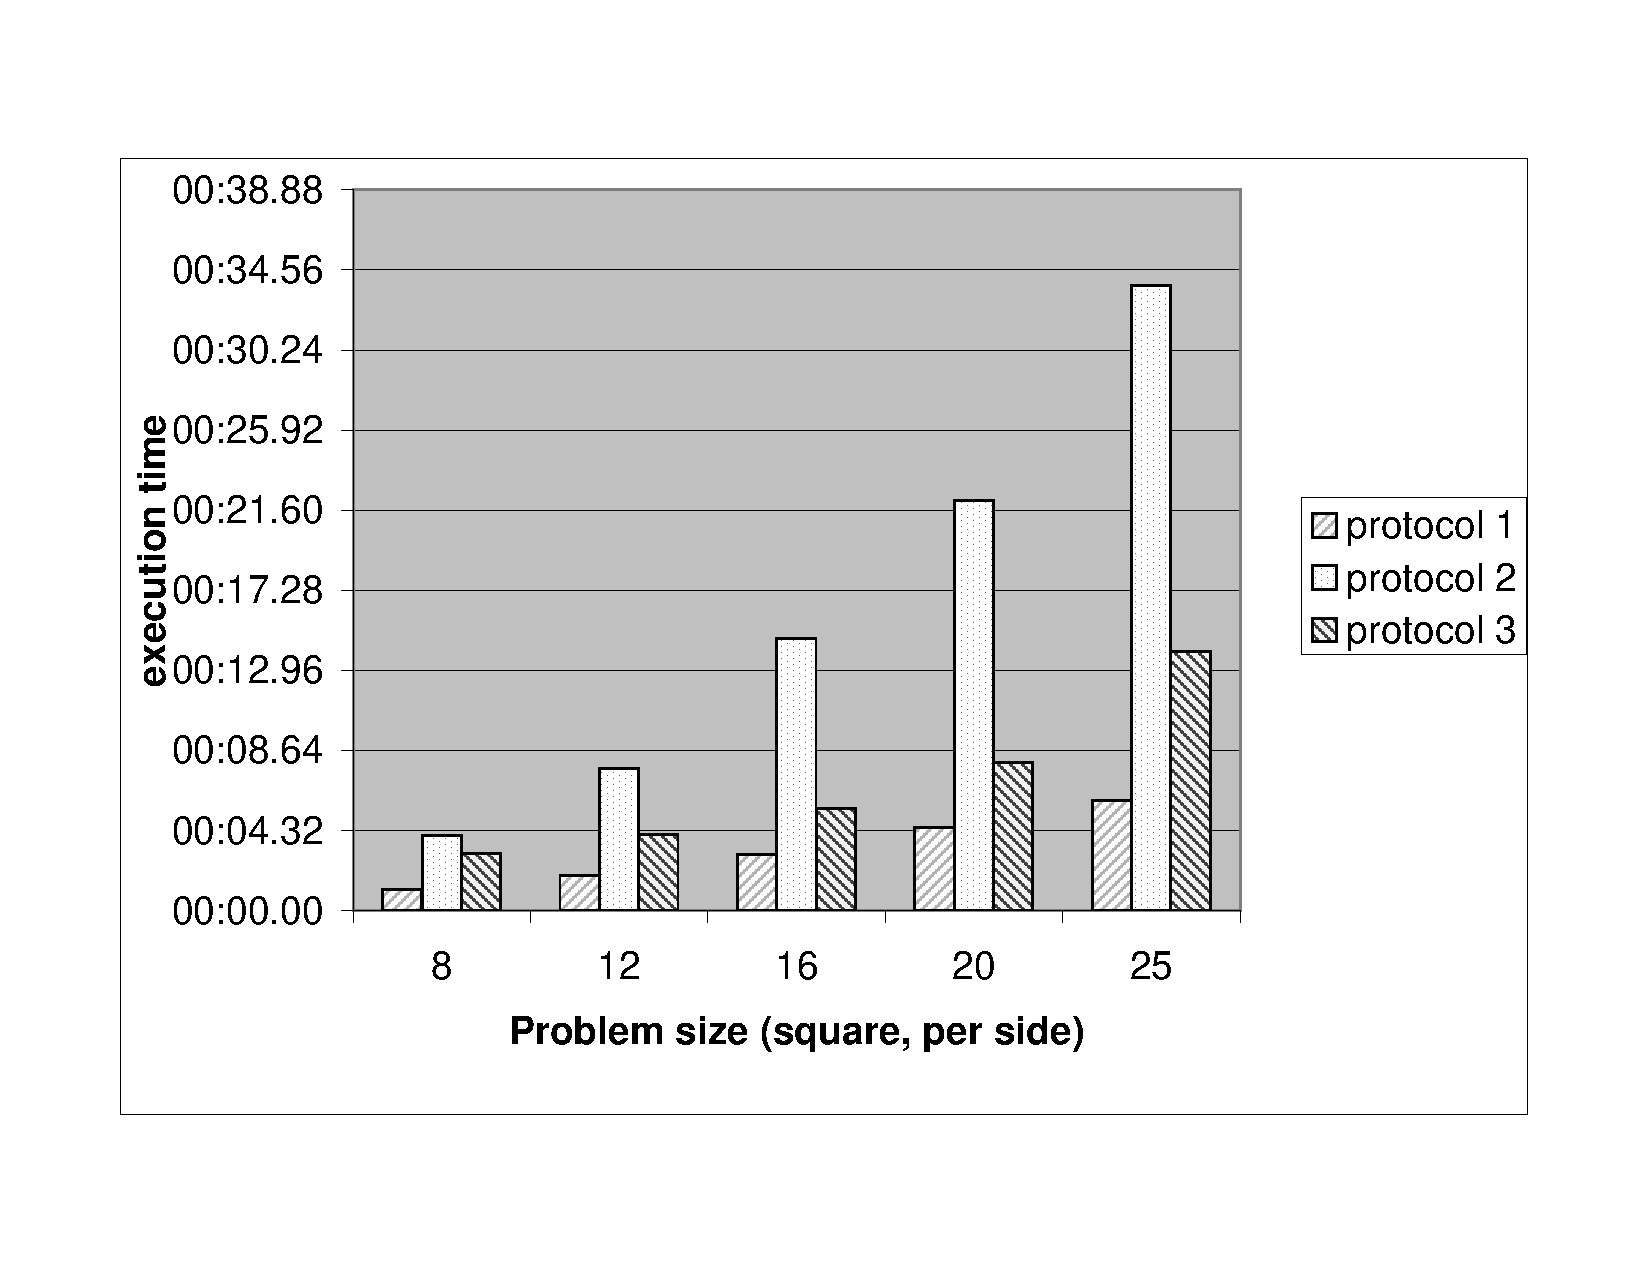
\includegraphics[bb=22bp -50bp 600bp 1000bp,scale=0.4,angle=0]{genomics/proto123}}
\caption{Timing measurements (in minutes and seconds) comparing protocols
1, 2, and 3. The Atallah~\cite{atallah} protocol could not complete problems of
sizes $(25,25)$ and $(25,25)$.}
\label{fig:histogram} 
\end{figure*}

Detailed results for protocol $1$ and $2$ are presented in the
appendix.  We discuss results for Protocol $3$ in detail. Recall that
in this protocol a grid structure is used (see
section~\ref{subsec:protocol3}).  Using Protocol $3$, we were able to
solve problems instances of considerable size; here we present
measurements for a problem instance of size
(200,200). Table~\ref{protocol3table200} shows the results using
various grid sizes. Performance steadily improves up to the grid size
of $20$, but begins to decrease slightly after that.  In spite of
decreased overall performance, further increases in the grid size
slightly decrease network bandwidth requirements, which results in
fewer round trips, so even larger grid sizes may be suitable for
environments with limited network bandwidth.  With a grid size of
$20$, Protocol 3 requires about as much time for an instance of size
$(200,200)$ as Protocol 2 requires for an instance of size ($25,25)$.


\subsection{Smith-Waterman}
\label{sec:sw-experimental}

For Protocols 1 and 3, the Yao circuit is modified by embedding the
cost function in the circuits. Recall that for edit distance, $\sigma=0$
if $\alpha[i]=\beta[j]$, $1$ otherwise. In Smith-Waterman, $\sigma$ is
an arbitrary cost function $c(u,v)$. The modified circuits effectively
perform a table lookup on $c(\alpha[i],\beta[j])$ in determining the
lowest cost alignment. Likewise, the gap function, which is a constant $1$
for edit distance, is replaced by the gap value of the scoring function
for Smith-Waterman. By convention, lower numbers represent higher costs
(higher numbers represent a similarity score) so a maximum-of-three circuit is
used instead of min-of-3.

We also constructed a protocol for Smith-Waterman based on Protocol
2. Recall that in Protocol $2$ for edit distance, a circuit for
equality of the characters is evaluated. For Smith-Waterman, an
$OT_{\mid \Sigma \mid}^{1}$ is performed instead. Alice, acting as the sender,
creates an array with a row of the cost function subtracted from her
random share $r$.  Each element of the array is $r-c(\alpha[i],\beta)$
for each possible $\beta\in\Sigma$. Bob, acting as the chooser, selects
the element with index $\beta[j]$. In this way, Bob receives the value
$r-c(\alpha[i],\beta[j])$.  Alice and Bob's shares are then input into
a maximum-of-three circuit which computes the next value of the shared dynamic
programming matrix.  The remaining details of the protocol are the same
as for edit distance.


Figure~\ref{fig:sw-histogram} shows the timing measurements for the
three protocols.  For Protocols 1 and 3, the computation time scales
with the size of the score matrix, which is ${\mid \Sigma \mid}^{2}$. For
example, the bytes transferred over the network aligning protein
sequences using BLOSUM62 are approximately 40 times that of for simple
edit distance of the same size problem.  This is caused by the use of
extra gates in the Yao circuit which encode each value of the score
function.  For Protocol 2, the computation scales with the alphabet
size $\mid \Sigma \mid$. For a very large alphabet with hundreds of symbols,
Protocol $2$ would be the best choice because the cost of embedding
the entire matrix into a Yao circuit becomes prohibitive.

\begin{figure*}
\centerline{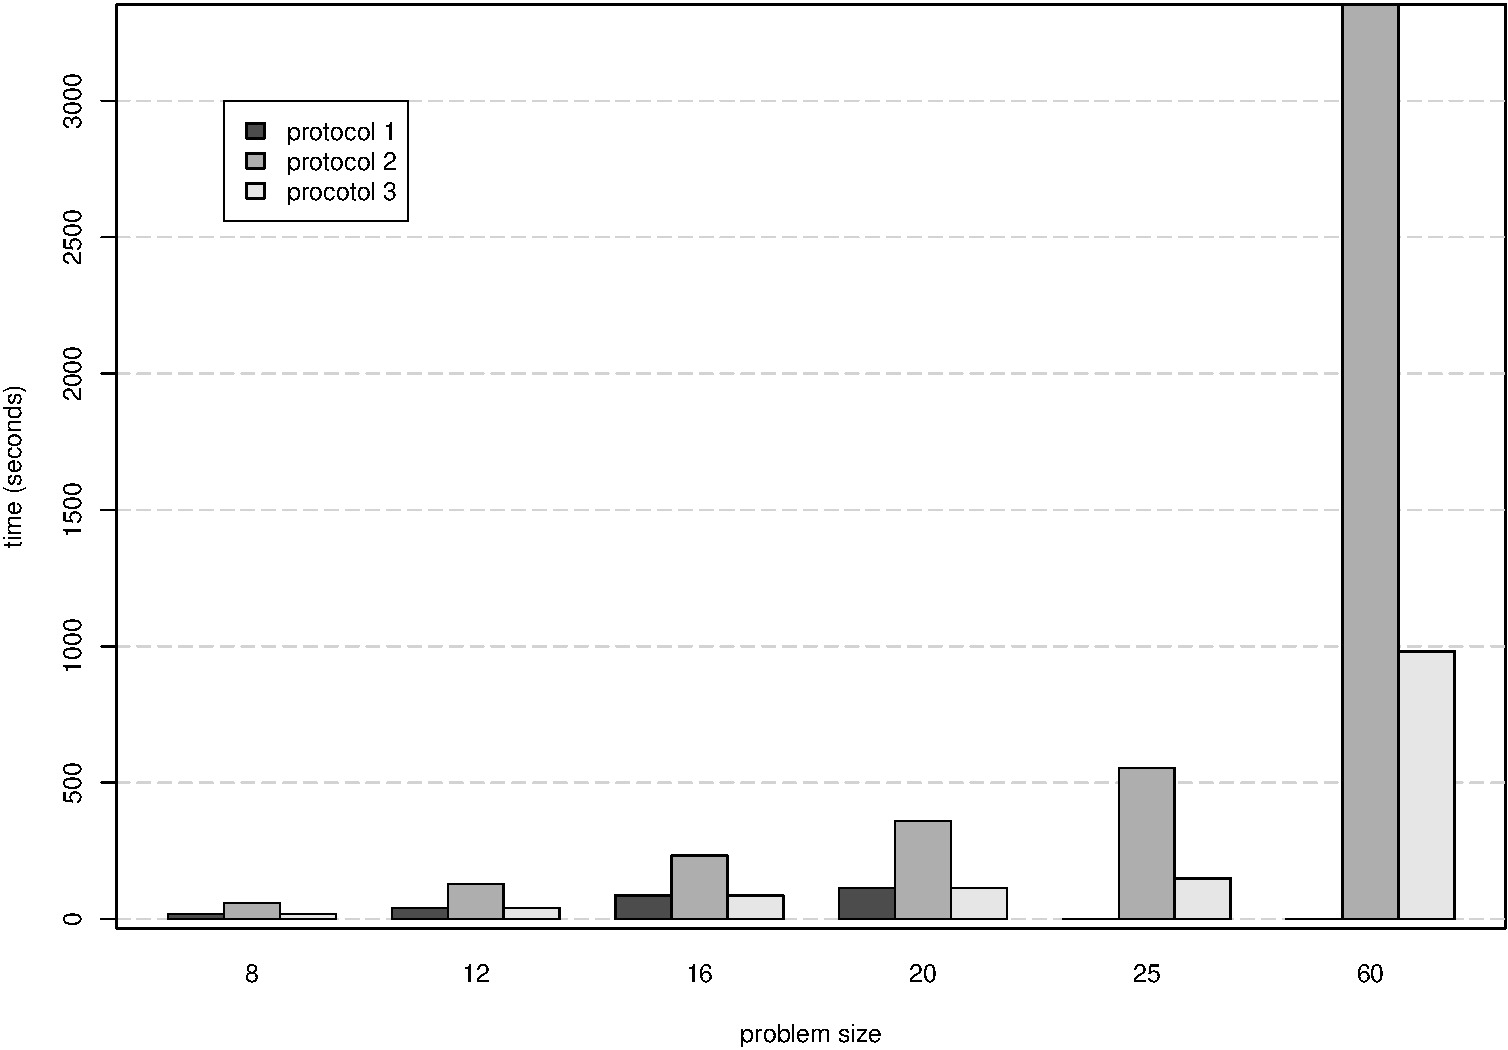
\includegraphics[scale=0.4,angle=0]{genomics/sw123}}

\caption{Timing measurements (in minutes and seconds) comparing Smith-Waterman
Protocols 1, 2, and 3. For problem sizes (25,25) and (60,60), Protocol
1 could not evaluate the circuit.}

\label{fig:sw-histogram} 
\end{figure*}

\begin{table}
\begin{centering}
\begin{tabular}{|c||c|c|c|c|c|}
\hline 
Grid size &
Bandwidth (Alice) &
Bandwidth (Bob) &
CPU (Alice) &
CPU (Bob) &
wall clock \tabularnewline
\hline
\hline 
25 &
362.2 M &
2.1 M &
518 &
84 &
658 \tabularnewline
\hline 
20 &
368.5 M &
2.6 M &
385 &
90 &
534 \tabularnewline
\hline 
10 &
397.4 M &
5.4 M &
476 &
123 &
655 \tabularnewline
\hline 
8 &
412.0 M &
5.8 M &
520 &
145 &
729 \tabularnewline
\hline 
4 &
485.3 M &
14.4 M &
784 &
234 &
1095 \tabularnewline
\hline 
2 &
635.2 M&
32.0 M&
1296 &
408 &
1804 \tabularnewline
\hline 
1&
948.0 M&
76.7 M&
2480 &
780 &
4883 \tabularnewline
\hline
\end{tabular}
\par\end{centering}

\caption{Network bandwidth (in bytes) and timing measurements (in seconds)
for edit-distance Protocol 3 with a problem of size $(200,200)$.
(M refers to Megabytes)}

\label{protocol3table200} 
\end{table}





\chapter{Conclusions}
In this thesis, we have looked at techniques for making secure function
evaluation practical. In chapter 4, we looked at the use of Ordered
Binary Decision Diagrams (OBDDs) to optimize the evaluation of certain
kinds of functions. Our conclusions were that OBDDs can provide a
significant performance gain for certain functions. In chapter 5,
we discussed a specialized use of SFE to solve the classic problem
of password authentication in a novel way. The solution presented
has useful properties that no existing solution has, and is fast enough
for practical use. Chapter 6 presented general techniques for applying
SFE to dynamic programming problems. The techniques presented are
of general algorithmic interest, but we applied these techniques to
traditional genomic algorithms and showed that efficient protocols
for computing edit distance and Smith-Waterman alignment scores can
be constructed. Chapter 7 presented another efficient protocol to
solve the K-means clustering problem, used in genomics and other machine
learning problems. In chapter 8, we delved into the cryptographic
primitives used in SFE and showed how modular square roots could be
used as an efficient trapdoor function for $1$ out of $N$ oblivious
transfer.

Our thesis statement was that SFE can be used to solve practical problems
today. We believe that this dissertation demonstrates by example that
SFE is ready to move from a curiosity of purely theoretical interest
into a technique that is ready for practical application today on
the internet.


%\bibliography{general,somesh,vitaly,misc,smithw}
%\appendix
%\begin{proof}
%\section{Proof of Lemma~\ref{lemma:circuit}}
\label{appendix:lemma}

The proof is by simultaneous induction on $l$ and $w$. For $l=1$ and
$w=1$ the results follows using the following recursive relationship:
\begin{eqnarray*}
D(i,j) & = & \mbox{min} [ D(i-1,j) + 1, D(i,j-1)+1, D(i-1,j-1)+t(i,j) ]
\end{eqnarray*}
The induction step is tedious but simple. Assume that the result is true for all $l'$ and $w'$ such that $l' \leq l$ and
$w' \leq w$.  We will prove the result that for $l+1$ and $w$. Recall that
we have to prove that $D(i,j)$, can be expressed as a function of ${\it
bottom}(D(i,j),l+1,w)$, ${\it left}(D(i,j),l+1,w)$, $ \alpha [ i-w+1
\cdots i ]$, and $\beta [ j-l \cdots j]$.  The following three statements are true
by induction hypothesis:
\begin{itemize}
\item $D(i-1,j)$ can be expressed as a function of ${\it
bottom}(D(i-1,j),l+1,w-1)$, ${\it left}(D(i,j),l+1,w-1)$, $ \alpha [ i-w+1
\cdots i-1 ]$, and $\beta [ j-l \cdots j]$

\item $D(i,j-1)$ can be expressed as a function of ${\it
bottom}(D(i,j-1),l,w)$, ${\it left}(D(i,j-1),l,w)$, $ \alpha [ i-w+1
\cdots i ]$, and $\beta [ j-l \cdots j-1]$

\item $D(i-1,j-1)$ can be expressed as a function of ${\it
bottom}(D(i-1,j-1),l,w-1)$, ${\it left}(D(i-1,j-1),l,w-1)$, $ \alpha [ i-w+1
\cdots i-1 ]$, and $\beta [ j-l \cdots j-1]$.
\end{itemize}
Notice that $D(i,j)$
can be expressed in terms of $D(i-1,j)$, $D(i,j-1)$, $D(i-1,j-1)$, 
$\alpha[i]$,  and $\beta[j]$. Now the result is clear by combining the
the four statements mentioned above. Similarly, we can prove that $D(i,j)$, can be expressed as a function of ${\it
bottom}(D(i,j),l,w+1)$, ${\it left}(D(i,j),l,w+1)$, $ \alpha [ i-w
\cdots i ]$, and $\beta [ j-l+1 \cdots j]$. $\Box$
\end{proof}

%\section{Detailed Results for Protocols $1$ and $2$}
\label{appendix:results} 



As a preparation step, a specific circuit must be constructed for each
problem instance.  We implemented a program which takes as its input a
description of the problem instance and outputs a description in the
Fairplay input language SHDL. Fairplay is able to take the SHDL
description and output a circuit. Table~\ref{protocol1table} shows the
network bandwidth (in bytes) and execution times (in seconds) for
various problem instances. For problems of size greater than (25,25),
the Fairplay compiler exhausted available memory and could not create
the circuit. In this experiment, the circuits operate using $8$-bit
integers bits, which allows for a maximum edit distance of 255. Results
for Protocol 2 can be found in Table~\ref{protocol2table}.

%
\begin{table*}
\begin{center}
\begin{tabular}{|c||c|c|c|c|c|} \hline 
Problem size & Bandwidth (Alice) & Bandwidth (Bob) & CPU (Alice) & CPU (Bob) & wall clock \\ \hline \hline 
(25,25)& 4.38M & 10472 & 4.26 & 1.17 & 5.94 \\ \hline 
(20,20)& 2.97 M & 8764 & 3.10 & 0.88 & 4.46 \\ \hline
(16,16) &1.83 M & 7057 & 2.12 & 0.68 & 3.02 \\ \hline
(12,12) & 0.96 M & 5348 & 1.30 & 0.54 & 1.92 \\ \hline 
(8,8) & 0.37 M & 3633 & 0.74 & 0.39 & 1.12 \tabularnewline
\hline
\end{tabular}
\end{center}


\caption{Network bandwidth (in bytes) and timing measurements (in seconds) for protocol 1. (M refers to Megabytes)}
\label{protocol1table}
\end{table*}

\begin{table*}
\begin{centering}
\begin{tabular}{|c||c|c|c|c|c|}
\hline 
Problem size &
Bandwidth (Alice) &
Bandwidth (Bob) &
CPU (Alice) &
CPU (Bob) &
wall clock \tabularnewline
\hline
\hline 
8x8 &
717 k &
68 k &
3.03 &
1.29 &
4.05 \tabularnewline
\hline 
12x12 &
1.60 M &
154 k &
5.96 &
2.37 &
7.68 \tabularnewline
\hline 
16x16 &
3.36 M &
315 k &
11.5 &
4.38 &
14.7 \tabularnewline
\hline 
20x20 &
5.26 M &
492 k &
17.5 &
6.54 &
22.1 \tabularnewline
\hline 
25x25 &
8.21 M &
769 k &
26.8 &
9.7 &
33.7 \tabularnewline
\hline 
100x100 &
171.1 M&
32.0 M&
519 &
177 &
649 \tabularnewline
\hline
\end{tabular}
\par\end{centering}


\caption{Network bandwidth (in bytes) and timing measurements (in seconds)
for edit-distance Protocol 2 with various problem sizes. (k and M
are kilobytes and megabytes respectively)}

\label{protocol2table} 
\end{table*}









%
\section{Comparison with the edit distance protocol of~\cite{atallah}}
\label{appendix-atallah}

In~\cite{atallah}, Atallah \emph{et al.} presented a privacy-preserving
edit distance protocol, which is superficially similar to our Protocol 2
in that the intermediate values $D(i,j)$ are additively shared between
Alice and Bob.  The protocol of~\cite{atallah} relies on different
cryptographic techniques, including special-purpose solutions to the so
called ``millionaires' problem'' (a two-party protocol, in which the
parties determine whose input is bigger without revealing the actual
input values) and additively homomorphic encryption.

In this section, we present a detailed comparison of the online
computational cost of our protocol vs.\ that of~\cite{atallah}.  Let $q
= \lceil \log w \rceil$ be the length of each alphabet symbol, and
let $s=\log(n+m)$ be the length of random shares used to mask $D(i,j)$
in our protocol.  In the protocol of~\cite{atallah}, masking is done by
adding random values under encryption, in a group of unknown order which
is much larger than $2^{n+m}$.  Therefore, this addition \emph{cannot}
be modular, and must be done over the integers.  To achieve standard
cryptographic security, the length of random shares in bits must be at
least $s'=\log(n+m)+80=s+80$.

Below, we compare the cost for a single iteration, since the number of
iterations is equal to $n \times m$ in both protocols.

\vspace{1ex}
\noindent
\textbf{Online computational cost of~\cite{atallah}.}
Each iteration uses the minimum or maximum finding protocol three times:
twice in step 1 on $q$-bit values, and once in step 5 on $s'$-bit
values~\cite[section 4.1]{atallah}.  Each minimum/maximum finding
protocol requires two instances of the millionaires' sub-protocol, and
six re-randomizations of Paillier ciphertexts.  The latter is done by
exponentiation modulo $N^2$, where $N^2$ is the modulus of an instance
of Paillier encryption scheme.  $N$ itself is an RSA modulus and must
be at least 1024 bits; therefore, $N^2$ is at least 2048 bits.

The implementations of the millionaires' protocol suggested
in~\cite{atallah} are relatively inefficient.  For fair comparison,
we will assume that the construction of~\cite{atallah} is instantiated
with a state-of-the-art sub-protocol for the millionaires' problem, \eg,
the Lin-Tzeng protocol~\cite{lintzeng-acns05}.  This protocol requires
$(1540 s' - 6)$ online modular multiplications per instance if $s'$-bit
values are being compared ($1540 q - 6)$ if $q$-bit values are being
compared), assuming the standard size of 512 bits for the prime moduli
in ElGamal encryption.

Assuming that the permutations required by~\cite{atallah} are free,
the online cost of each iteration is thus equivalent to
$2 \times (2 \times (1540 q - 6) + 6 \times 2048) +
          (2 \times (1540 s' - 6) + 6 \times 2048)$ =
$2 \times (3080 q - 12 + 12288) +
          (3080 s' - 12 + 12288)$ =
$3080s' + 6160q + 36828$ =
$3080s + 6160q + 283228$ modular multiplications.

\vspace{1ex}
\noindent
\textbf{Online computational cost of our Protocol 2.}

Each iteration of our Protocol 2 involves evaluation of several ``garbled
circuits.''  Each $\CE$ circuit has $2q$ gates of arity 2, and each
$\CM$ circuit has $10s$ gates of arity 2, and $5s-6$ gates of arity 3.
In each iteration, a single instance of $\CE$ and a single instance of
$\CM$ must be evaluated (in our presentation, evaluation of circuits $\CE$
and $\CM$ is split between two phases, but there is a 1:1 correspondence
between the iterations of each phase).

All garbled circuits can be pre-computed in advance, because the
representation of the circuit in Yao's protocol is independent of the
actual input values.  Each row of the truth table of each gate becomes
a double-encrypted symmetric ciphertext (see section~\ref{sub:Garbled-Circuit-Method}), for
a total of $4 \times 2 q + (4 \times 10s +  8 \times (5s - 6))$ = $8q
+ 80s - 48$ ciphertexts.  Decrypting each double-encrypted ciphertext
requires two online symmetric decryptions, but, on average, the evaluator
of a garbled gate will only need to try decrypting half the ciphertexts
before decryption succeeds and he obtains the wire key representing the
bit value of the gate's output wire.

Transferring the wire-key representation of Bob's $q$-bit input into $\CE$
requires $q$ instances of $OT_1^2$.  The online cost of each instance using Pinkas-Naor OT
(see section~\ref{sub:Oblivious-Transfer})
is 2 modular exponentiations for the sender and 1 modular exponentiation for the chooser.  Therefore,
assuming 512-bit moduli, the total online cost of obliviously transferring
the inputs to $\CE$ is equivalent to $1025q$ modular multiplications.

In the same iteration, a single instance of $\CM$ must be evaluated.
Bob has three $s$-bit inputs (after evaluating $\CE$, he already has
the representation for his fourth input).  Obliviously transferring
the wire-key representation of these inputs requires $3s$ instances of
$OT_1^2$, for a total cost of $3075 s$ modular multiplications.

Therefore, the total online cost of each iteration of our Protocol
2 is $(3075 s + 1025 q)$ modular multiplications and $8q + 80s -
48$ symmetric decryptions vs.\ $(3080 s + 6160 q + 283228)$ modular
multiplications in each iteration of~\cite{atallah}.  Since symmetric
decryption is much cheaper than modular multiplication, we conclude
that our Protocol 2 offers significantly better efficiency than the
protocol of~\cite{atallah}.  In general, the protocol of~\cite{atallah}
requires \emph{at least} 300,000 modular multiplications per iteration,
rendering it unrealistically expensive for practical applications.


%\section{Security Proofs}

\newcommand{\view}{\mathsf{view}}
\newcommand{\sot}{S^\mathsf{ot}}
\newcommand{\mot}{S^\mathsf{min}}

Our protocols are secure in the so called the \emph{semi-honest} model
of secure computation, \ie, under the assumption that both participants
faithfully follow the protocol specification.  To achieve security in
the \emph{malicious} model, where participants may deviate arbitrarily
from protocol specification, participants would need to commit to their
respective inputs prior to protocol start and then prove in zero knowledge
that they follow the protocol specification.  

Since we use Yao's ``garbled circuits'' method as the underlying
primitive, security in the malicious model, if needed, can be achieved as
at constant cost~\cite{JS07}.  For practical usage scenarios, however, it
is not clear whether security in the malicious model offers significant
advantages over security in the semi-honest model.  For example, there
is no external validation of the parties' inputs.  Even if the protocol
forces each party to run the protocol on previously committed inputs,
this does not guarantee that the inputs are not maliciously chosen in
the first place.  In other words, a malicious party may simply commit
to a ``bad'' input (deliberately chosen so that the result of the edit
distance computation reveals some information about the other party's
input) and pass all proofs.

In general, we expect that our protocols will be used for tasks such as
collaborative analysis of genome sequence in joint medical studies, where
it is reasonable to assume that participants provide actual sequences
as inputs into the protocol, and are not deliberately supplying fake
sequences in an attempt to learn something about the other participant's
data.

Security of Protocol 1 follows directly from (i) security of subprotocols
performed using standard methods for secure multi-party computation,
and (ii) composition theorem for the semi-honest model~\cite[Theorem
7.3.3]{Goldreich:vol2}.  Proofs are standard and omitted for brevity.

Security of Protocol 2 is proved via a standard simulation in the
semi-honest model.  For each protocol participant, we demonstrate the
existence of an efficient simulator algorithm which, with access to
this participant's input and output, produces a simulation which is
computationally indistinguishable from this participant's ``view'' of
the protocol (informally, a ``view'' is a record of sent and received
messages).

Let $\view_A(\alpha)$ (respectively, $\view_B(\beta)$) be Alice's
(respectively, Bob's) view of the protocol when executed on input string
$\alpha$ (respectively, $\beta$).  Each party's view consists of its
respective input as well as all messages received by this party in the
course of the protocol.  The output of the protocol is the edit distance
$\delta(\alpha,\beta)$.  Because edit distance is a deterministic function
of the parties' inputs, to prove security of the protocol it is sufficient
to construct simulators $S_A$ and $S_B$ such that
\[
\begin{array}{rcl}
\{S_A(\alpha,\delta(\alpha,\beta))\} 
& \stackrel{c}{\equiv} &
\{\view_A(\alpha)\} \\
\{S_B(\beta,\delta(\alpha,\beta))\} 
& \stackrel{c}{\equiv} &
\{\view_B(\beta)\}
\end{array}
\]
Here $\stackrel{c}{\equiv}$ stands for computational
indistinguishability~\cite{GoldreichBookVol1}.

As the building blocks for our simulator, we will use the simulators for
Yao's ``garbled circuits'' protocols for evaluating the $\CE'$ and $\CM$
circuits.  The difference between $\CE'$ and $\CE$ is that, unlike $\CE$,
which outputs the wire key representing the result of equality testing
(as opposed to the actual result), $\CE'$ outputs a single bit $\sigma$:
$0$ if the values are equal, $1$ if they are not (\ie, $\CE'$ is the
standard equality testing circuit).

% Because the oblivious transfer protocol is assumed to be secure, there
% exist simulators $\sot_A,\sot_B$ such that, for $i\in\{0,1\}$:
% \[
% \begin{array}{rcl}
% \{\sot_A(i,x_i)\} 
% & \stackrel{c}{\equiv} &
% \{\view^{\mathsf{ot}}_A(i)\} \\
% \{\sot_B(x_0,x_1,\perp)\} 
% & \stackrel{c}{\equiv} &
% \{\view^{\mathsf{ot}}_B(x_0,x_1)\}
% \end{array}
% \]
% where $x_0,x_1$ are Bob's inputs into the $OT_1^2$ protocol,
% $i$ is Alice's choice ($0$ or $1$), $\perp$ is the ``empty'' output
% (it denotes that Bob does not receive any output from the protocol), and
% $\view^{\mathsf{ot}}_A$ and $\view^{\mathsf{ot}}_B$ are, respectively,
% Alice's and Bob's views of the $OT_1^2$ protocol.

Security of the protocol for computing the $\CM$ circuit implies that
there exist simulators $\mot_A,\mot_B$ such that:
\[
\begin{array}{rcl}
\{\mot_A(x_1,x_2,x_3,r)\} 
& \stackrel{c}{\equiv} &
\{\view^{\mathsf{min}}_A(x_1,x_2,x_3,r)\} \\
\{\mot_B(y_1,y_2,y_3,t,z)\} 
& \stackrel{c}{\equiv} &
\{\view^{\mathsf{min}}_B(y_1,y_2,y_3,t)\} \\
\multicolumn{3}{l}{
\mbox{where } z=\min(x_1 \oplus y_1 + 1,x_2 \oplus y_2 + 1,x_3 \oplus y_3+t) \oplus r
}
\end{array}
\]

The simulators for the parties' respective views of $\CE'$ are similar.


\paragraph{Simulating Alice's view.}
Simulation of Alice's view in Phase 0 is trivial.

In Phase 1, Alice participates in multiple instances of secure
evaluation of circuits $\CE$.  By security of Yao's ``garbled circuits''
protocol~\cite{LP04}, there exist simulators for Alice's views of every
instance of $\CE'$.  Since Alice's view of $\CE$ is exactly the same as
her view of $\CE'$ (the only difference between the two circuits is their
respective outputs for Bob), our simulator simply invokes the simulator
for $\CE'$ to simulate Alice's view of each instance.

Phase 2 consists of $n \times m$ iterations, one for each value of the
$(i,j)$ pair.  Therefore, Alice's $\view_A$ of Protocol 2 is a composition
of Alice's views of individual iterations $\view_A^{(i,j)}$.

For all $(i,j)$ where either $i \neq n$, or $j \neq m$, $\view_A^{(i,j)}$
is simply her view of the secure evaluation protocol for the circuit
$\CM$.  To simulate Alice's view of the $\CM$ evaluation on the $(i,j)$
instance, the simulator simply invokes the sub-simulator $\mot_A$ for
this protocol.  Note that Alice receives no output from $\CM$.

Finally, $\view_A^{(n,m)}$ contains an additional message $m_B$ from
Bob at the very end of the protocol, which in the real execution
enables Alice to reconstruct the output of the entire protocol,
\ie, $\delta(\alpha,\beta)$.  Because the simulator has access to
$\delta(\alpha,\beta)$, it simulates $m_B$ as $\delta(\alpha,\beta)-r_A$,
where $r_A$ is Alice's fourth input into the $\CM$ circuit in the
$(n,m)$ iteration.  Observe that in both the simulation and the real
execution, the sum of $r$ and $m_B$ is equal to $\delta(\alpha,\beta)$.
This completes the simulation of Alice's view.


\paragraph{Simulating Bob's view.}
Simulating Bob's view is a little more difficult.  The simulator
maintains an internal table $M: \{0,1\}^r \rightarrow \{0,1\}$.
In Phase 1, for each instance of circuit $\CE(i,j)$, our simulator
invokes the sub-simulator for Bob's view of $\CE'(i,j)$ on Bob's input
$\beta[j]$.  The output of the sub-simulator is the bit $\sigma(i,j)$,
which represents whether $\alpha[i]=\beta[j]$ or not.  

The simulator generates a random $r$-bit value $k(i,j)$, stores the
mapping $M(k(i,j))=\sigma(i,j)$ in its internal table $M$, and sends
$k(i,j)$ to Bob.  Now, in the real evaluation of $\CE$, Bob receives an
$r$-bit wire key.  Because wire keys are generated uniformly at random,
the simulated value $k(i,j)$ has exactly the same distribution as the
real wire key, and Bob cannot distinguish between the key from the real
execution and the simulation.

In Phase 2, for each instance of circuit $\CM(i,j)$, the simulator runs
on Bob's input $k(i,j)$, which is equal to the same random value that the
simulator returned to Bob when simulating $\CE(i,j)$.  Bob's inputs are
$D_B(i-1,j)$,$D_B(i,j-1)$,$D_B(i-1,j-1)$, and $k(i,j)$.  Our simulator
invokes the sub-simulator $\mot_B(D_B(i-1,j),D_B(i,j-1),D_B(i-1,j-1),
M(k(i,j)))$.  Observe that the fourth argument is the result of looking
up $\sigma(i,j)$ corresponding to $k(i,j)$ in the simulator's internal
table $M$.  Recall that $\sigma(i,j)$ is the result of the comparison
between $\alpha[i]$ and $\beta[j]$.  The output of $\mot_B$ is returned
to Bob.

Finally, $\view_B^{(n,m)}$ contains an additional message $m_A$ from
Alice at the very end of the protocol, which in the real execution
enables Bob to reconstruct the output of the entire protocol,
\ie, $\delta(\alpha,\beta)$.  Because the simulator has access to
$\delta(\alpha,\beta)$, it simulates $m_A$ as $\delta(\alpha,\beta)-r_B$,
where $r_B$ is the output of the $\mot_B$ sub-simulator in the $(n,m)$
iteration.

Indistinguishability of Bob's real and simulated views follows from the
existence of simulators for $\CE'$ and $\CM$, and the fact that Bob
cannot tell the difference between a wire key generated by Alice (in
the real protocol) and a ``fake'' value of the same length generated
randomly by the simulator (in the simulated protocol), since both are
random values are drawn from the same distribution.

% This sub-simulator requires the actual
% minimum value as one of its inputs.  The simulator substitutes a random
% value $r''$ for the actual minimum.  As in any protocol for securely
% evaluating function $f(x,y)$ where Alice and Bob hold random shares of
% $x$ and $y$~\cite{Goldreich:vol2}, Alice's share of the result is random
% and independent of $f(x,y)$.  Therefore, the substitution is undetectable.





\chapter{Oblivious Transfer with Modular Square Roots}\label{sec:OT-SquareRoots}
\label{chapter:otquad}

A new $OT_{2}^{1}$ protocol is presented, using the square root function
in modular multiplicative groups as a trapdoor function. Here, I present
a informal sketch of correctness, security, and efficiency. I propose
to complete the proofs and perform a thorough experimental evaluation
of its performance with respect to other oblivious transfer protocols.


\section{Protocol}
\begin{enumerate}
\item The sender chooses large random prime numbers $p$ and $q$ such that
$p\equiv q\equiv3\;(\mbox{mod }4)$ and calculates $n=pq$. $n$ is
sent to the chooser. This is a one time setup step that need not be
repeated for subsequent uses of the protocol.
\item The chooser uniformly chooses a random value $x\in S\subset Z_{n}^{*}$
where $S=\{z\in Z_{n}^{*}:$~$z\le\frac{n-1}{2}\mbox{ and }$ $\left(\frac{z}{n}\right)=-1$
if $s=1$ otherwise $\left(\frac{z}{n}\right)=+1\}$. The chooser
computes $y\equiv x^{2}(\mbox{mod }n)$ and sends $y$ to the sender.
$\left(\frac{x}{n}\right)$ denotes the Jacobi symbol of $x$ and
$n$.
\item The sender calculates the square roots $a^{2}\equiv b^{2}\equiv y\;(mod\, n)$
such that $\left(\frac{a}{n}\right)=-1$ and $\left(\frac{b}{n}\right)=+1$
and $a,b\le\frac{n-1}{2}$
\item The sender encrypts $E_{a}(m_{1})$ and $E_{b}(m_{2})$ and sends
them to the chooser.
\item The chooser computes $D_{x}(E_{x}(m_{s}))$ to decrypt the output.
\end{enumerate}

\section{Correctness}

$\left(\frac{x}{n}\right)=-1$ for half the elements $x\in Z_{n}^{*}$
. $\left(\frac{x}{n}\right)=+1$ for the other half. Thus the chooser
can always successfully perform step 2.

If $a^{2}\equiv b^{2}\;(mod\; n)$ and $a\neq\pm b\;(mod\; n)$ then
$\left(\frac{a}{n}\right)=-\left(\frac{b}{n}\right)$.%
\footnote{This follows when $p\equiv q\equiv3\ (\mbox{mod 4})$ from the properties
of the Jacobi symbol and the Chinese Remainder Theorem.%
} Furthermore, the set $\{a,b,n-a,n-b\}$is the complete set of square
roots of $y$. If $a>\frac{n-1}{2}$ then $a$ and $n-a$ can be swapped,
and similarly for $b$. Thus, the sender can always successfully complete
step 3. It is guaranteed that either $a=x$ or $b=x$ so the chooser
will successfully learn $m_{s}$ as intended.


\section{Security}

Finding all square roots of any quadratic residue in $Z_{n}^{*}$
can be reduced to factoring $n$. This is because given two principal
square roots $a^{2}\equiv b^{2}$, $a\neq-b$, then $(a-b)(a+b)\equiv0$
so $(a-b)(a+b)=kpq$ Under the standard complexity assumption that
factoring $n$ is infeasable, then the chooser can not efficiently
learn the other square root of $x^{2}$, which is the encryption key
of $E(m_{3-s})$ and the sender's privacy is preserved. 

The chooser's privacy is preserved because the sender does not know
whether the chooser calculated $y=a^{2}$ or $y=b^{2}$. From the
sender's perspective, the chooser has chosen $x$ from a uniform random
distribution $1\le x\le\frac{n-1}{2}$, so there is no information
that can be gained. The chooser therefore enjoys unconditional security
even without making assumptions about the senders computation power.


\section{Efficiency}

In the setup phase, the sender needs to calculate $n=pq$ once and
send the value of $n$ to the chooser. This requires one multiplication
and transmission of $k=\log n$ bits. The same value of $n$ can be
reused for subsequent or batched OTs without loss of security. $k$
must be large enough to prevent efficient factoring of $n$.

From then on, each OT requires the following: 
\begin{enumerate}
\item Computation of Jacobi symbols $\left(\frac{x}{n}\right)$ by the chooser.
If the chooser uses random trials to find an appropriate $x$, then
the expected number of trials is $2$. Computing Jacobi symbols can
be performed in $O(k\log x)\le O(k^{2})$ steps \cite{1996-bach-book}. 
\item There is a potential optimization of step 1. The chooser can pre-compute
a single number $\alpha$ where $\left(\frac{\alpha}{n}\right)=-1$.
From then on, the chooser can choose any random $\beta$ and have
$\left(\frac{\beta^{2}}{n}\right)=+1$ and $\left(\frac{\alpha\beta^{2}}{n}\right)=-1$.
This optimization as presented is insecure, because it breaks statistical
indistinguishability for the chooser~%
\footnote{The optimization will never produce a non-QR with $+1$ Jacobi symbol%
}. However, I speculate that there may exist a variation which avoids
this flaw and thereby reduces the chooser's overall complexity to
$O(k)$.
\item Transmission of a single $k$ bit number from chooser to sender
\item Computation by the sender of square roots of $y$. This can be performed
using a randomized algorithm in expected time $O(k\ \log\, p^{2})\le O(k^{3})$
steps for $p>q$ \cite{1996-bach-book}. 
\item Encryption and transmission by the sender of the two messages. If
the sender does not need to hide the length of the unreceived message,
then this requires no more bandwidth than the actual size of the messages,
which is $O(\log m)$
\item Decryption by the receiver of one of the messages, which is $O(\log m)$.
\end{enumerate}
If the sender and chooser wish to execute the protocol multiple times,
the chooser can simply send a vector $[y_{1},\cdots,y_{j}]$ and the
chooser will respond with a vector of tuples $[(E_{a_{1}}(m_{1_{1}}),(E_{b_{1}}(m_{1_{2}}))\cdots(E_{a_{j}}(m_{j_{1}}),(E_{b_{j}}(m_{j{}_{2}}))]$
where $j$ is the number of messages to be sent obliviously. Each
$x_{i}$ is an independent random variable so the security is equivalent
to the single message case. Thus, unlimited bits can be transferred
with a single network round-trip.


\section{Comparison with Naor-Pinkas\label{sub:Comparison-with-Naor-Pinkas}}

In the Naor-Pinkas protocol \cite{Noar-Pinkas:2001}, the computational
requirement for each party is $O((\log n)(\log\log n))$ for both
parties, where $n$ is the size of a group sufficiently large such
that calculating discrete logarithms is infeasible. The communication
consists of a message of size $\log n$ from sender to chooser, a
message of size $\log n$ from chooser to sender, and two messages
of size $\log m+\log n$ from sender to chooser, where $\log m$ is
the size of the chooser's outputs. The protocol presented here cuts
the final messages to $\log m$, which effectively reduces the bandwidth
with a tradeoff in computation time. My experimentation with running
SFE algorithms using fast modern CPUs indicates that this tradeoff
may be worthwhile. I plan to make empirical measurements with implementations
of the to comparitively measure the actual performance.


\section{Extensions}

It may be possible to extend the construction to cover the more general
$OT_{k}^{1}$. I have not investigated this yet, but one idea is to
let $n=\prod_{i=1}^{k}p_{i}$ where each $p_{i}$ is a large prime
number. In $Z_{n}^{*}$, each quadratic residue will have $2^{k}$
square roots consisting of $2^{k-1}$ pairs $(x,n-x)$

%
\begin{comment}
\bibliographystyle{plain}
\bibliography{crypto,privacy,somesh}

\end{comment}
{}




\chapter{Private Information Retrieval}
%Secure function evaluation is practical.


\chapter{K-means clustering}
\label{chapter:kmeans}

%% Importance of privacy
%% cite laws and popular articles

\section{Contribution}
The previous chapter introduced our work in privacy-preserving
genomics by presenting algorithms for dynamic programming such
as the Smith-Waterman sequence alignment.  In this chapter,
we present a privacy preserving algorithm for clustering, an
unsupervised learning algorithm used in genomics and many other
machine-learning domains.

%% Contributions of this paper

This chapter makes the following contributions:

\begin{itemize}
\item We present the design and analysis of privacy-preserving $k$-means
clustering algorithm for horizontally partitioned data (see
Section~\ref{sec:k-means}). The crucial step in our algorithm is
privacy-preserving of cluster means. We present two protocols for
privacy-preserving computation of cluster means. The first protocol is
based on oblivious polynomial evaluation and the second one on
homomorphic encryption. These protocols are described in detail in
Section~\ref{sec:WAP}.

\item We present an open-source implementation of our algorithm. 
We believe that modular design of our implementation will enable other
researchers to use our implementation.  We evaluated the two privacy-preserving
clustering algorithms on real data sets. Our first conclusion is that
privacy-preserving clustering is feasible. For example, for a large
data set ($5,687$ samples and $12$ features) from the speech
recognition domain our homomorphic-encryption-based algorithm took
approximately $66$ seconds. We also observed that both in bandwidth
efficiency and execution overhead algorithms based on homomorphic
encryption performed better than the one based on oblivious polynomial
evaluation. A detailed discussion of our evaluation is given in
Section~\ref{sec:eval}.

\end{itemize}



\section{Related work}

As discussed in the previous chapter,
emphasis has been placed on preserving the
privacy of user-data aggregations, e.g., databases of personal
information.  Access to these  collections is, however, enormously
useful.  It is from this balance between privacy and utility that the
area of {\it privacy preserving data-mining}
emerged~\cite{Agrawal-Srikant,Lindell-Pinkas}.


%% Clustering description

Unsupervised learning deals with designing classifiers from a set of
unlabeled samples. A common approach for unsupervised learning is to
first cluster or group unlabeled samples into sets of samples that are
``similar'' to each other. Once the clusters have been constructed, we
can design classifiers for each cluster using standard techniques
(such as decision-tree
learning~\cite{Mitchell:AI,Quinlan:86}). Moreover, clusters can also
be used to identify features that will be useful for
classification. There is significant research on privacy-preserving
algorithms for designing
classifiers~\cite{Agrawal-Srikant,Lindell-Pinkas}. This paper
addresses the problem of privacy-preserving algorithms for clustering.


%% Problem description

Assume that Alice $A$ and Bob $B$ have two unlabeled samples $D_A$ and
$D_B$. We assume that each sample in $D_A$ and $D_B$ has all the
attributes, or the data sets are horizontally partitioned between $A$
and $B$. Alice and Bob want to cluster the joint data set $D_A \cup
D_B$ without revealing the individual items of their data sets (of
course Alice only obtains the clusters corresponding to her data set
$D_A$). In this paper, we assume that clustering the joint data set
$D_A \cup D_B$ provides better results than individually clustering
$D_A$ and $D_B$.  Using a large data set from the networking domain we also demonstrate
that clustering the joint data set results in significantly different
clusters than individually clustering the data sets (see end of
section~\ref{sec:eval} for details). We present a privacy-preserving
version of the $k$-means algorithm where only the cluster means at the
various steps of the algorithm are revealed to Alice and Bob.


%% Applications of clustering to medical informatics
%% and intrusion detection

There are several applications of
clustering~\cite{pattern-classification}. Any application of
clustering where there are privacy concerns is a possible candidate
for our privacy-preserving clustering algorithm. For example, suppose
network traffic is collected at two ISPs, and the two ISPs want to
cluster the joint network traffic without revealing their individual
traffic data. Our algorithm can be used to obtain joint clusters while
respecting the privacy of the network traffic at the two ISPs. An
application of clustering to network intrusion detection is presented
by Marchette~\cite{Marchette99}.  Clustering has been used for
forensics~\cite{Pouget:Dacier} and root-cause analysis for
alarms~\cite{Julisch:TISSEC}. Clustering has also been used in
bioinformatics. For example, Dhillon {\it et al.}~\cite{Dhillon:Bio}
have used clustering to predict gene function. We believe that
privacy-preserving clustering can be used in bioinformatics where the
data sets are owned by separate organizations, who do not want to
reveal their individual data sets.




In general, there are two approaches for designing privacy-preserving
machine learning algorithms. The first approach is to use
transformations to perturb the data set before the algorithm is
applied. This approach for designing privacy-preserving clustering
algorithms is taken by several
researchers~\cite{Klusch,MeruguGhosh,Oliveira}. A second approach to
designing privacy preserving algorithms is to use algorithms from the
secure-multiparty computation literature. The advantage of this
approach over the perturbation approach is that formal guarantees of
privacy can be given for these algorithms. Our thesis takes the latter
approach. Vaidya and Clifton~\cite{VaidyaClifton} present a
privacy-preserving $k$-means algorithm for vertically-partitioned data
sets, whereas our thesis considers
clustering for horizontally-partitioned data. Vaidya and Clifton's
algorithm is based on the secure-permutation algorithm of Du and
Atallah~\cite{DuAtallah}. However, Vaidya and Clifton's algorithm has
to execute Du and Atallah's protocol for every item in the data
set. Therefore, their algorithm is not practical for large data sets.
Moreover, Vaidya and Clifton did not perform an experimental
evaluation of their algorithm.  By contrast, the complexity of our
algorithm only depends on the number of steps taken by the $k$-means
algorithm and the dimension of the data items. There are distributed
clustering algorithms where the goal is to reduce communication
costs~\cite{DhillonModha,Kargupta}.  These distributed clustering
algorithms do not consider privacy.

In our implementation, we approximate real numbers using intervals
(see section~\ref{sec:approximating-reals}).  Finite-precision
approximation to functions may leak information. Feigenbaum {\it et
al.}~\cite{Nissim:2001} show that approximations to functions can be
made private by adding noise.



\section{The $k$-means clustering algorithm}
\label{sec:k-means}

The $k$-means algorithm~\cite{pattern-classification,Llyod-82} is
shown in Figure~\ref{fig:k-means}. Assume that we are given $n$
samples $x_1,\cdots,x_n$, where each sample is a $m$-dimensional
vector of real numbers. The number of clusters is $c$. The algorithm
maintains $c$ means $\mu_1,\cdots,\mu_c$. Initially, assume that the
means are assigned arbitrary values. A sample $x_i$ is deemed to be in
the cluster $j$ if it is closest to the mean $\mu_j$, where mean of a
cluster $\{x'_1,\cdots,x'_r \}$ is
$\frac{x'_1+\cdots,x'_r}{r}$. Distance between two $m$-dimensional
vectors $x$ and $y$ is given by $\sum_{j=1}^m (x[j] - y[j])^2$, where
$x[j]$ is the $j$-th element of the vector $x$.  Other distance
metrics~\cite[Chapter 10]{pattern-classification}, such as scatter
metrics, can be used instead of the distance metric mentioned above.
Each iteration of the $k$-means algorithms recomputes the means and
reclassifies the samples. The algorithm terminates when it detects
``no change'' in the means. The precise definition of ``no change''
depends on the specific metric being used. We also assume that the
initial cluster means are chosen randomly. There is some research on
picking the initial cluster means~\cite{Initial:kmeans}. Various
techniques for picking initial cluster means can be easily
incorporated into our algorithm. This issue will not be discussed
further in the paper.


\begin{figure}
\begin{center}
\begin{programbox}
\mbox{Algorithm ($k$-means clustering)}
\BEGIN \mbox{initialize $n,c,\mathbf{\mu}_1,\cdots,\mathbf{\mu}_c$}
	\DO \mbox{classify $n$ samples according to nearest $\mathbf{\mu}_i$, and }
	    \mbox{recompute $\mathbf{\mu}_i$}
	\mbox{{\bf \underline{until}} no change in $\mathbf{\mu}_i$'s}
 \mbox{{\bf \underline{return}} $\mathbf{\mu}_1,\mathbf{\mu}_2,\cdots,\mathbf{\mu}_c$}
\END
\end{programbox}
\end{center}
\caption{The $k$-means clustering algorithm.}
\label{fig:k-means}
\end{figure}

\subsection{Distributed $k$-means}

Assume that Alice $A$ (party $1$) has $z$ samples $\{
x_1,\cdots,x_{n_A} \}$, and Bob $B$ (party $2$) has $n-n_A$ samples
$\{ x_{n_A + 1},\cdots,x_n \}$. Each party wants to jointly cluster
their samples without revealing any private information. We are
assuming that clustering the union of samples from the two parties is
more desirable than clustering the two samples individually.

Assume that there is a trusted third party $TTP$. $A$ and $B$ perform
iterations locally. However, at each iteration the new cluster means
$\mathbf{\mu}_i$s are computed by communicating with the $TTP$. Let
$C_i^A$ and $C_i^B$ be the cluster corresponding to mean
$\mathbf{\mu}_i$ for $A$ and $B$, respectively.  $A$ sends $c$-pairs
$\langle (a_1,b_1), \cdots, (a_c,b_c) \rangle$ to $TTP$, where $a_i =
\sum_{x_j \in C_i^A } x_j$ and $b_i = \mid C_i^A \mid$ ($a_i$ is the sum of
samples in cluster $C_i^A$ and $b_i$ is the number of samples in the
cluster $C_i^A$). Analogously, $B$ sends $c$-pairs $\langle (d_1,e_1),
\cdots, (d_c,e_c) \rangle$ to the $TTP$, where $d_i = \sum_{x_j \in
C_i^B } x_j$ and $e_i = \mid C_i^B \mid$. The $TTP$ computes the $c$
means $\langle \mu_1, \cdots, \mu_c \rangle$ and sends them to $A$ and
$B$, where $\mu_i = \frac{a_i+d_i}{b_i+e_i}$. We call this algorithm
{\em distributed $k$-means} or $D_{\mbox{$k$-means}}$.

\subsection{Assumptions}

Our goal is to design a privacy-preserving $k$-means that does not
use a TTP. Before we present such an algorithm, we state assumptions
made in the design of our  privacy-preserving algorithm.

\paragraph{Number of parties.} In this paper we only present the
two party case. 

\paragraph{The adversary model.} We assume a  semi-honest
adversary (also called honest but curious adversary model)~\cite{Goldreich:vol2}.
There are standard constructions that transform a protocol that
is secure in the semi-honest model and produce a protocol that is
secure in a more general malicious model (these constructions are
called ``semi-honest to malicious'' compilers, and details of these
constructions can be found in~\cite{Goldreich:compiler:99}).

\paragraph{Information disclosure.} Our privacy-preserving algorithm
discloses the cluster means at the various steps to the two parties.
Therefore, the computation of classifying samples according to the
nearest cluster means can be performed locally. Therefore, the
complexity of our privacy-preserving algorithm depends only on the
number of steps taken by the $k$-means algorithm and the
number of features, but not on the size of the data. This is a desirable property
because usually the data sets to be clustered can be very large.

\subsection{Privacy-preserving $k$-means}

In order, to create a privacy-preserving version of $k$-means that does
not use a TTP we have to devise a privacy-preserving protocol to
compute the cluster means. Consider the computation of a single
cluster mean $\mu_i$. Recall that in distributed $k$-means each
party sends $(a_i,b_i)$ and $(d_i,e_i)$ to the TTP, which computes
$\frac{a_i+d_i}{b_i+e_i}$; this is precisely the function for which
we have to devise a privacy-preserving protocol. This problem can be
formally defined as follows:

\begin{definition}
\rm
The {\em weighted average problem (WAP)} is defined as follows:
party $1$ has a pair $(x,n)$, where $x$ is a real number and $n$ is
a positive integer. Similarly, party $2$ has pair $(y,m)$. They want
to jointly compute $\frac{x+y}{n+m}$. In other words, we need a 
privacy-preserving protocol for the following functionality:
\begin{eqnarray*}
((x,n),(y,m)) & \longmapsto & (\frac{x+y}{n+m}, \frac{x+y}{n+m})
\end{eqnarray*}
The notation shown above means that the first and second party provide
inputs $(x,n)$ and $(y,m)$ to the protocol and both parties receive
output $\frac{x+y}{n+m}$. Notice that WAP is different than the classical
problem of computing the averages, where $n$ parties have a number and 
they jointly want to compute the average without revealing their individual
numbers. In the classical problem, the number of parties $n$ is known
to all the parties. In WAP, the number of points $n$ and $m$ needs to
be kept secret. 
\end{definition}

Let ${\cal P}_{WAP}$ be a privacy-preserving protocol for solving
WAP. Two protocols for WAP are presented in Section~\ref{sec:WAP}.  In
the privacy-preserving $k$-means algorithm (denoted as
$PP_{\mbox{$k$-means}}$) $A$ and $B$ use ${\cal P}_{WAP}$ instead of
the trusted third party $TTP$ to compute the cluster means
$\mathbf{\mu}_i$s.  The algorithm is shown in
Fig~\ref{fig:pp-k-means}. We only show the part of the algorithm
executing at Alice's (party $1$) side. Bob (party $2$) will execute a
similar algorithm at his side.

\noindent
{\bf Note:} Suppose that the initial clusters are picked randomly. For
the privacy-preserving algorithm we need a protocol for two parties to
jointly pick a common random vector. Such a protocol is called {\it
coin-tossing into the well} and is based on commitment schemes
(see~\cite[Section 7.4.3.1]{Goldreich:vol2}).

\begin{figure}
\begin{center}
\begin{programbox}
\mbox{Algorithm $PP_{\mbox{$k$-means}}$ (privacy-preserving $k$-means clustering)}
\BEGIN \mbox{initialize $n_A ,c,\mathbf{\mu}_1,\cdots,\mathbf{\mu}_c$}
	\DO \mbox{classify $n_A$ samples according to nearest $\mathbf{\mu}_i$}
	    \FOR i := 1 \TO c \STEP 1 \DO
	     \mbox{Let $C_i^A$ be the $i$-th cluster}
	     \mbox{Compute $a_i = \sum_{x_j \in C_i^A } x_j$ and $b_i = \mid C_i^A \mid$}
	     \mbox{recompute $\mathbf{\mu}_i$ by invoking the protocol ${\cal P}_{WAP}$ }
	    \OD
	\mbox{{\bf \underline{until}} no change in $\mathbf{\mu}_i$}
 \mbox{{\bf \underline{return}} $\mathbf{\mu}_1,\mathbf{\mu}_2,\cdots,\mathbf{\mu}_c$}
\END
\end{programbox}
\end{center}
\caption{The privacy-preserving $k$-means clustering algorithm.}
\label{fig:pp-k-means}
\end{figure}

\subsection{Proof of Privacy}

In this section we provide a proof of privacy for the protocol shown
in Figure~\ref{fig:pp-k-means}.  The proof uses a semi-honest
adversary model. Notice that in the distributed $k$-means algorithm
$\mathcal{D}_{\mbox{$k$-means}}$ both parties only know their input
and output.  Definition of privacy is based on the intuition that
parties should learn nothing more from the messages used in
privacy-preserving protocol, i.e., the messages received by a party
during an execution of a privacy-preserving protocol can be
``effectively computed'' by only knowing its input and output. This
idea is formalized below:

\begin{definition}
\label{def:privacy}
\rm
Let $x$ and $y$ be inputs of the two parties and $\langle f_1 (x,y),
f_2 (x,y) \rangle$ be the desired functionality, i.e., the first party
wants to compute $f_1 (x,y)$ and the second wants to compute $f_2
(x,y)$. Let $\Pi$ be a two-party protocol to compute $f$. The view
of the first party after having participated in protocol $\Pi$ 
(denoted by $\mbox{VIEW}_1^\Pi (x,y)$) is $(x,r,m_1, \cdots m_t)$, where
$r$ are the random bits generated by party $1$ and $m_1, \cdots, m_t$ is the
sequence of messages received by party $1$, while participating in protocol
$\Pi$. The view $\mbox{VIEW}_2^\Pi (x,y)$ for the second party  is defined
in an analogous manner.

We say that $\Pi$ {\em privately computes} $f$ if there exists 
probabilistic polynomial-time algorithms (PPTA), denoted by $S_1$ and $S_2$
such that

\begin{eqnarray*}
\{ S_1 (x,f_1 (x,y)) \}_{x,y} & \equiv^s & \{ \mbox{VIEW}_1^\Pi (x,y) \}_{x,y} \\
\{ S_2 (x,f_2 (x,y)) \}_{x,y} & \equiv^s & \{ \mbox{VIEW}_2^\Pi (x,y) \}_{x,y} \\
\end{eqnarray*}

In the equation given above, $\equiv^s$ denotes {\em statistically
indistinguishable}.  Two probability ensembles $X = \{ X_w \}_{w \in
S}$ and $Y = \{ Y_w \}_{w \in S}$ indexed by $S$ are statistically
indistinguishable if for some negligible function $\mu : \aleph \mapsto
[0,1]$ and all $w \in S$,
\begin{eqnarray*}
\sum_{\alpha} \mid Pr ( X_w = \alpha ) - Pr ( Y_w = \alpha ) \mid & < & \mu ( \mid w \mid )
\end{eqnarray*}
A function $\mu : \aleph \mapsto [0,1]$ is called {\it negligible}
if for every positive polynomial $p$, and all sufficiently large $n$'s,
$\mu (n) < \frac{1}{p(n)}$. There is a weaker notion of indistinguishability
called {\em computationally indistinguishable}. We will use statistical
indistinguishability throughout the paper, but all the results hold even if
the weaker notion of indistinguishability is used. Detailed definitions of
these concepts can be found in~\cite{GoldreichBookVol1,Goldreich:vol2}. 

\end{definition}

The privacy-preserving $k$-means algorithm uses the privacy-preserving
protocol ${\cal P}_{WAP}$ for the WAP. Assume that the two parties
invoke the protocol ${\cal P}_{WAP}$ as an oracle, i.e., both parties
write their respective inputs (in this case $(x,n)$ and $(y,m)$) and
invoke the oracle which returns the result (in this case
$\frac{x+y}{n+m}$). Recall that in the distributed $k$-means
algorithms both parties learn the cluster means at various steps. If
we use oracle calls to compute the cluster means, then the two parties
also learn only the cluster means. So the views in the two cases are
{\it identical}.  Hence, the conditions of
definition~\ref{def:privacy} are trivially satisfied. However, there
are additional messages exchanged in the protocol ${\cal P}_{WAP}$
used to compute the cluster means. We need to ensure that nothing can
be learned from these messages. The privacy of protocol shown in
Figure~\ref{fig:pp-k-means} follows from the composition
theorem~\cite{CanettiComposition} stated below ($g$ is the algorithm
shown in Figure~\ref{fig:pp-k-means} and $f$ is the protocol ${\it
P}_{WAP}$ to solve WAP described in Section~\ref{sec:WAP}):

\begin{theorem}
\label{thm:composition}
{\rm (Composition Theorem for the semi-honest model):}
Suppose that $g$ is privately reducible to $f$ and that there exists a protocol
for privately computing $f$. Then there exists a protocol for privately
computing $g$.
\end{theorem}




\section{Privacy-Preserving Protocol for \\ the Weighted Average Problem}
\label{sec:WAP}

In the weighted average problem (WAP) we want to find
a privacy-preserving protocol for the following functionality:
\begin{eqnarray*}
((x,n),(y,m)) & \longmapsto & (\frac{x+y}{n+m}, \frac{x+y}{n+m})
\end{eqnarray*}
Recall that a protocol for WAP was used in
the privacy-preserving $k$-means algorithm (see Figure~\ref{fig:pp-k-means}).


A simple strategy to address this problem is to first approximate the
function $\frac{x+y}{n+m}$ by a circuit $C$, and then use standard
constructions~\cite{Goldreich87,Goldreich:JACM:91,Yao86} to construct
a privacy-preserving protocol.  Protocols constructed using this
strategy have a very high computational overhead. Malkhi {\it et al.} 
considered the cost of implementing these protocols in their work in
the Fairplay system~\cite{mnps04}.  They found that the protocol was
feasible for small circuits, e.g., a single $\wedge$-gate could be
implemented in $410$ milliseconds, and more complex integer numerical
functions could be implemented on the order of seconds.  They further
showed the runtimes of these protocols grow quickly with the size of
the input and complexity of the implemented function.  The most
complex function discussed by the authors computed a median of two
ten-element integer input sets.  This function took over $7$ seconds
to execute in a LAN environment, and over $16$ seconds in an WAN
environment.  The circuit for computing $\frac{x+y}{n+m}$ is
significantly more complex. Hence, with a non-trivial data set, a
single computation of cluster means may take several minutes to compute.  Note that
the underlying costs of Fairplay are not artifacts of the design, but
simply the cost of implementing the standard protocols; the reported
costs were almost completely dominated with circuit setup and the
necessary oblivious transfers.

In this section, we present two privacy-preserving protocols for WAP
that are more efficient than the standard protocols. The first
protocol is based on oblivious polynomial evaluation and the second on
homomorphic encryption. Similarity of WAP with a problem that occurs
in protocols for generation of shared RSA
keys~\cite{Boneh-Franklin-2001,Gilboa99} is discussed in
appendix~\ref{sec:shared-RSA}.


\subsection{Protocol based on oblivious polynomial evaluation}
\label{subsec:OPE}

We will first give a privacy-preserving protocol for a general problem,
and then at the end of the subsection demonstrate how we can construct
a privacy-preserving protocol for WAP.  Consider the following
problem.

\begin{definition}
\rm
Let ${\cal F}$ be a finite field. Party $1$ has two polynomials $P$
and $Q$ with coefficients in ${\cal F}$. Party $2$ has two points
$\alpha$ and $\beta$ in ${\cal F}$. Both parties want to compute
$\frac{P(\alpha)}{Q(\beta)}$. In other words, we want to privately
compute the following functionality:
\begin{eqnarray*}
((P,Q),(\alpha,\beta)) & \longmapsto & (\frac{P(\alpha)}{Q(\beta)},\frac{P(\alpha)}{Q(\beta)})
\end{eqnarray*}
We call this problem {\em private rational polynomial evaluation (PRPE)}.
\end{definition}

The protocol $\mathcal{P}_{PRPE}$
uses a protocol for oblivious polynomial evaluation, which is defined below.

\begin{definition}
\rm
Let $\mathcal{F}$ be a finite field.  The {\em oblivious polynomial
evaluation} or {\em OPE} problem can be defined as follows: Alice
$A$ has a polynomial $P$ over the finite field $\mathcal{F}$, and
Bob $B$ has an element $x \in \mathcal{F}$. After executing the  protocol
implementing OPE $B$ should {\em only know} $P(x)$ and $A$ should
know nothing.
\end{definition}

A protocol to solve the OPE was  given by Naor and
Pinkas~\cite{NaorPinkas99}.  Let $\mathcal{P}_{OPE}(P,\alpha)$ denote
the privacy-preserving protocol for OPE. We provide a protocol
$\mathcal{P}_{PRPE}((P,Q),(\alpha,\beta))$ for PRPE, which uses
$\mathcal{P}_{OPE}(P,\alpha)$ as an oracle. The protocol is shown in
Figure~\ref{fig:PRPE}. 

\begin{figure}
\framebox{\parbox[c]{6.5in}{
{\bf (Step 1)} Party $1$ picks a random element $z \in \mathcal{F}$ and
computes two new polynomials $zP$ and $zQ$. In other words,
party $1$ ``blinds'' the polynomials $P$ and $Q$.
\medskip\\
{\bf (Step 2)} Party $2$ computes $z P(\alpha)$ and $z Q(\alpha)$ by
invoking the protocol for OPE twice, i.e., invokes the 
protocol $\mathcal{P}_{OPE}(zP,\alpha)$ and $\mathcal{P}_{OPE}(zQ,\beta)$.
\medskip\\
{\bf (Step 3)} Party $2$ computes $\frac{P(\alpha)}{Q(\beta)}$ by computing
$\frac{z P(\alpha)}{z Q(\beta)}$ and sends it to party $1$.
}}
\caption{Protocol for PRPE.}
\label{fig:PRPE}
\end{figure}


\begin{theorem}
\rm
\label{thm:privacy-PRPE}
Protocol $\mathcal{P}_{PRPE}((P,Q)(\alpha,\beta)$ shown in Figure~\ref{fig:PRPE}
is privacy-preserving protocol for PRPE.
\end{theorem}
{\bf Proof:} The views of the two parties are
\begin{eqnarray*}
\mbox{VIEW}_1^{\mathcal{P}_{PRPE}} (P,Q) & = & (P,Q,\frac{P(\alpha)}{Q(\beta)}) \\
\mbox{VIEW}_2^{\mathcal{P}_{PRPE}} (\alpha,\beta) & = & (\alpha,\beta, z P(\alpha), z Q(\beta))
\end{eqnarray*}
The view of party $1$ consists of its input $(P,Q)$ and output $\frac{P(\alpha)}{Q(\beta)}$.
Therefore, there is nothing to prove (see definition~\ref{def:privacy}, we can use
$S_1$ as the identity function). The input and
output of party $2$ are $(\alpha,\beta)$ and $\frac{P(\alpha)}{Q(\beta)}$ respectively.
We have to show a PPTA $S_2$ such that
$S_2 (\alpha,\beta,\frac{P(\alpha)}{Q(\beta)})$ and $\mbox{VIEW}_2^{\mathcal{P}_{PRPE}} (\alpha,\beta)$
are statistically indistinguishable. Let $z'$ be a random element of $\mathcal{F}$ and $S_2 (\alpha,\beta,\frac{P(\alpha)}{Q(\beta)})$
be defined as follows:
\[
(\alpha,\beta, z' \frac{P(\alpha)}{Q(\beta)},z')
\]
It is easy to see that the following two ensembles are statistically indistinguishable:
\[
\begin{array}{l}
(\alpha,\beta, z' \frac{P(\alpha)}{Q(\beta)},z') \\
(\alpha,\beta, z P(\alpha), z Q(\beta))
\end{array}
\]
The reason is that if $z$ is a random element of $\mathcal{F}$ then $z
Q(\beta)$ is a random element of $\mathcal{F}$ as well. Moreover, the
ratio of the third and fourth elements in the view of party $2$ is
$\frac{P(\alpha)}{Q (\beta)}$, i.e., the output and the third element
of the view determine the fourth element of the view.

Recall that $\mathcal{P}_{PRPE}$ uses the protocol $\mathcal{P}_{OPE}$.
Using the composition theorem we conclude that $\mathcal{P}_{PRPE}$ 
is privacy preserving.
$\Box$

\paragraph{Protocol for WAP.} First, we show that a protocol $\mathcal{P}_{PRPE}$ for PRPE can be
used to solve WAP. Recall that in WAP party $1$ and party $2$ have inputs
$(x,n)$ and $(y,m)$ respectively. In the invocation of $\mathcal{P}_{PRPE}$, party $1$
constructs two polynomials $P(w) = w + x$ and $Q(w) = w + n$, and party $2$
sets $\alpha = y$ and $\beta = m$. The output both parties receive is equal
to $\frac{x+y}{n+m}$, which is the desired output. The proof of privacy
for this protocol follows from Theorem~\ref{thm:privacy-PRPE} and the composition
theorem.


\subsection{Protocol based on homomorphic encryption}
\label{subsec:homomorphic}

Let $(G,E,D,M)$ be a encryption scheme (where $G$ is the function to
generate public parameters, $E$ and $D$ are the encryption and
decryption functions, and $M$ is the message space respectively) with
the following properties:
\begin{itemize}
\item The encryption scheme $(G,E,D)$ is {\em semantically secure}~\cite{Goldwasser:Micali}.
Essentially, an encryption scheme is semantically secure
if an adversary gains no extra information by inspecting the ciphertext.
This is formally defined in the appendix (see definition~\ref{def:semantic-secure}).


\item  For all $m \in M$ and $\alpha \in M$, $m_1 \in E(m)$
implies that $m_1^\alpha \in E(m \alpha)$. Encrypting the same
message twice in a probabilistic encryption function can
yield a different ciphertext, so $E(m)$ denotes the set of
ciphertexts that can be obtained by encrypting $m$.\footnote{
Of course, to successfully decrypt  two different messages
$m$ and $m'$ sets $E(m)$ and $E(m')$ should be disjoint.}

\item There is a computable function $f$ such that for all messages $m_1$ and $m_2$
the following property holds:
\begin{eqnarray*}
f(E(m_1),E(m_2)) & = & E (m_1+m_2)
\end{eqnarray*}
\end{itemize}
There are several encryption scheme that have the three properties
mentioned above~\cite{Benaloh:94,Naccache-Stern,Paillier99}. In our
implementation, we used the {\it dense probabilistic encryption (DPE)}
scheme of Benaloh~\cite{Benaloh:94}. The semantic security of the
scheme provided by Benaloh is based on the intractability of 
deciding prime residuosity.



Party $1$ and $2$
have a pair of messages $(x,n)$ and $(y,m)$. The two parties want to
jointly compute $\frac{x+y}{n+m}$ in a privacy-preserving way. Assume
that party $1$ sets up a probabilistic encryption scheme $(G,E,D,M)$, and
publishes the public parameters $G$. We also assume that the probabilistic
encryption scheme $(G,E,D,M)$ satisfies the three properties given at the
beginning of the section. The protocol $\mathcal{P}_H$ for WAP is shown
in Figure~\ref{fig:protocol-homomorphic}.

\begin{figure}
\framebox{\parbox[c]{6.5in}{
\begin{itemize}
\item {\bf (Step 1)} Party $1$ encrypts $x$ and $n$ and sends the encrypted values $x_1 \in E(x)$
and $n_1 \in E(n)$ to party $2$.

\item {\bf (Step 2)} Party $2$ computes a random message $z \in M$, and encrypts $z \cdot y$ and $z \cdot m$ to obtain $z_1 \in E(z \cdot y)$
and $z_2 \in E(z \cdot m)$.
Party $2$ computes the following two messages and sends it to party $1$:
\begin{eqnarray*}
m_1 & = & f(x_1^z,  z_1) \\
m_2 & = & f(n_1^z, z_2) \\
\end{eqnarray*}
{\bf Note:} In our implementation we use the homomorphic-encryption scheme by~\cite{Benaloh:94} 
where $f$ is multiplication.

\item {\bf (Step 3)} Using the two properties of the probabilistic encryption scheme $(G,E,D)$,
we have the following:
\begin{eqnarray*}
m_1 & = & E(z \cdot x + z \cdot y) \\
m_2 & = & E(z \cdot n + z \cdot m) \\
\end{eqnarray*}
Therefore, party $1$ can compute $ z (x+y)$ and $z (n+m)$, and hence can compute
$\frac{x+y}{n+m}$. Party $1$ sends $\frac{x+y}{n+m}$ to party $2$. 
\end{itemize}
}}
\caption{Protocol for WAP based on homomorphic encryption.}
\label{fig:protocol-homomorphic}
\end{figure}

\begin{theorem}
\label{thm:privacy-homomorphic}
\rm
Assume that the probabilistic encryption scheme $(G,E,D)$ has three
properties mentioned at the beginning of this
sub-section. $\mathcal{P}_H((x,n),(y,m))$ is a privacy-preserving
protocol to compute$\frac{x+y}{n+m}$.
\end{theorem}
The proof of this theorem is straightforward and is given in
appendix~\ref{appendix:definitions-proofs}. The basic intuition is
that party $2$ cannot tell the difference between $E(x)$ and $E(n)$
and encryption of two arbitrary messages.

The complexity of encryption and decryption operations of a scheme
$(G,E,D,M)$ depends on size of the message space $M$. Therefore, in
order to keep the complexity low it is important that the size of the
message space be small. However, in order to achieve adequate
precision the message space should be large. Chinese remainder theorem
(CRT) allows us to perform computation over smaller spaces and then
reconstruct the result for a larger message space. Let
$p_1,\cdots,p_m$ be $m$ small primes.  The two parties execute the
protocol described above for $Z_{p_1}, \cdots, Z_{p_m}$. Party $1$
receives $z (x+y)$ and $z (n+m)$ modulo $p_i$ (for $1 \leq i \leq
m)$. CRT allows party $1$ to reconstruct $z (x+y)$ and $z (n+m)$
modulo $N \; = \; \prod_{i=1}^m p_i$. This technique is also used by
Gilboa~\cite{Gilboa99}.












\section{Implementation and Experiments}
\label{sec:eval}

This section looks at the feasibility of our solution by evaluating
the cost of the protocol on real data-sets.  The goal of this study is
to establish the cost of our privacy-preserving clustering algorithms
on real applications. We principally seek to understand the
performance and privacy tradeoffs inherent to the operation of the
protocols.

We evaluated three clustering algorithms. The {\it simple} scheme is
used throughout as a baseline for our experiments.  This protocol
implements the $k$-means clustering algorithm as described in
section~\ref{sec:k-means}.  This algorithm does not use any
privacy-preserving protocols.  This represents the nominal cost of
clustering, and will be present in any $k$-means clustering approach,
independent of if and how privacy is implemented.  Throughout this
section {\it features} refer to the dimension of the vectors being
clustered and each iteration of the $k$-means algorithm is referred to
as {\it round}.  Our first privacy-preserving protocol (referred to as
{\it OPE}) uses oblivious polynomial evaluation. This protocol is
described in detail in Section~\ref{subsec:OPE}.  For oblivious
polynomial evaluation we use the protocol presented by Naor and
Pinkas~\cite{NaorPinkas99}. The next privacy-preserving protocol
(referred to as {\it DPE}) uses homomorphic encryption scheme of
Benaloh~\cite{Benaloh:94}. This protocol is described in detail in
Section~\ref{subsec:homomorphic}.  

\paragraph{Implementation.}
Our system consists of approximately $3000$ lines of Java code, split
up into a number of self-contained modules.  The $k$-means algorithm
module implements actual clustering computations as described in
Section 3.  During each iteration, this module calls the {\small\sf
protocol} module to compute the cluster means for each dimension of
the cluster.  The {\small\sf protocol} module sets up the framework of
communication, and calls the specific protocol handlers with a common
interface, depending on which protocol is selected. In the {\it
simple} handler, Alice sends $(x,n)$ to Bob, who computes the cluster
mean $\frac{x+y}{n+m}$ and sends it to Alice.  The OPE and DPE
protocol handlers implement the protocols described in
Sections~\ref{subsec:OPE} and~\ref{subsec:homomorphic}.

The central results uncovered by this investigation include:

\newcommand{\itembase}{\setlength{\itemsep}{-3pt}}

\begin{enumerate}
\itembase

\item
Clustering using DPE is two orders of magnitude more bandwidth
efficient than OPE, and executes in 4.5 to 5 times less time.  This is
largely due to bandwidth and computational costs associated with the
oblivious transfers used by OPE.

\item 
Our protocols clustering with perfect fidelity; that is, the clusters
resulting from our algorithms are identical to those reported by a
$k$-means algorithm with no privacy for reasonable parameter choices.

\item
Small, medium, and large data-sets can be clustered efficiently.

\item
Costs scale linearly with feature and rounds.  The number of samples
affects run-time only inasmuch as it increases the number of rounds
toward convergence.

\item
Protocol parameters affect bandwidth usage by constant factor.
Moreover, exponential increases in security or supported message space
result in linear increases in execution run-times.

\end{enumerate}

\noindent
We begin in the following section by exploring several real data-sets
representative of expected environments.

\subsection{Experimental Data}
\label{sec:exdata}

The validity of our experimental approach is partially dependent on
the realism of our test data.  For this reason, we have obtained a
collection of externally provided data-sets representing diverse
applications.  All experiments described in this section use the
{\it synthetic}, {\it river}, {\it robot}, and {\it speech} data-sets
detailed below.

We selected the elements of our {\it synthetic} data-set to enable
testing and measure startup costs.  This data set includes 4 points
uniformly distributed within a 6 dimensional space.  By design, the
data clusters quickly into 4 "natural" clusters within 2 rounds under
the $k$-means algorithm in all experiments.

Originally used in the Computation Intelligence and Learning
(COIL) competition, the {\it river} data-set describes 
measurements of river chemical concentrations and algae
densities~\cite{coil99}.  The river data was used to ascertain the
summer algae growth of river water in temperate climates.  The
clustered data is used to inform the relationship between the presence
and concentrations of various chemicals in public waterways and algae
growth.  The river contains 184 samples with 15 features per sample.

The {\it robot} data-set~\cite{pion98} contains continuous senor
readings from the Pioneer-1 mobile robot used for testing computer
learning and conceptual development approaches.  Each of the 697
samples contains 36 features from sensor arrays of the Pioneer-1
mobile robot.  The samples were taken every 100ms and reflect the
movements and changing environment in which the robot was tested.  The
data has been clustered in prior use to recognize experiences with
common outcomes.

The {\it speech} data-set~\cite{jvow00} documents the measured voice
characteristics of spoken Japanese vowels.  Nine male speakers uttered
two Japanese vowels $/ae/$ repeatedly.  Sampled at 10kHz, the 640
utterances resulted in 12 features of 5,687 samples.  This large
data-set is used in the context of our experiments to evaluate the
degree to which the proposed protocols scale with the size of the
input data.  Similar data-sets are clustered frequently to help guide
speech recognition software~\cite{kts99}.

Each of the data-sets represents a singular corpus.  In contrast, our
protocols are targeted for applications of clustering with two
parties.  We model the two party case by randomly subdividing the
samples into equal sized subsets and assigning them to each party.  In
real environments the size of the sets may be vastly different.
Our approximation approach ensures that this kind of asymmetry will be
transparent to both parties both in execution and performance.  That
is, the performance of the algorithm is largely independent of the
number of samples.  However, as we shall see below, the number
of features has tremendous effect on the cost of clustering.

The last data set (called the {\it ping} data-set) was collected by
us. The purpose of collecting this data was two fold:
\begin{itemize}
\item Test our clustering algorithm on a large data set. 
\item Construct a data set that can be naturally partitioned to demonstrate that
jointly clustering two data sets can produce significantly different
results than individually clustering them. 
\end{itemize}
We setup two hosts
(referred to as $A$ and $B$) to measure ICMP ping round-trip
times. There were $4$ ping targets located around the world (one of
the ping targets was on the same subnet as host $B$). On each host and
for each ping target the pings were grouped in blocks of $200$. For
each block, a $3$-tuple consisting of the following three values was
generated: the average time to live (TTL), the average round-trip time
(RTT), and fraction of lost packets (\%drop). We collected data over a
period of $24$ hours and generated a data set consisting of $23872$
data points, which were evenly divided between host $A$ and $B$. We
ran our clustering algorithm on the joint data set, and data sets
corresponding to hosts $A$ and $B$. 



\subsection{Experimental Setup}
\label{sec:exsetup}

We use the architecture and code described earlier for the
experiments described throughout.  All experiments are executed on a
pair of 3Ghz machines with 2 gigabyte physical memory.  The
experimental application is running on the Sun Microsystems Java
Virtual Machine version 1.5~\cite{sun04} on the Tao Linux version 1.0
operating system~\cite{tao04}.  The protocols are executed on a
100Mbps unloaded LAN with a measured round-trip time of 0.2
milliseconds.

\begin{comment}
Unless otherwise stated, the reported measurements represent the
averages taken over 100 experiments.
\end{comment}

The experiments profile the additional cost of providing privacy in
clustering sensitive data.  To this end, we focus on three metrics of
cost and utility; {\it communication overhead}, {\it delay}, and {\it
precision}.  Communication overhead records the amount of additional
network bandwidth used by the privacy schemes over the simple schemes.
Delay measures the additional time required to complete the
clustering.

Precision is used to measure the degree to which the approximated
clustering diverge from those reported by a simple $k$-means
algorithm, and is calculated as follows.  Let $X = \{x_1, \dots,
x_n\}$ be the sample data set to be clustered.  $C_1 \subseteq 2^X$ is
the clustering of $X$ by the simple algorithm, and $C_2 \subseteq 2^X$
is the clustering returned by the OPE algorithm (the DPE metric is
defined similarly in the obvious manner).  For each pair $(x_i,x_j)$
such that $1 \leq i < j \leq n$ an error occurs if

\vspace{-4pt}

\itembase
\begin{enumerate}
\itembase
\item 
$x_i$ and $x_j$ are in the same cluster in $C_1$, but in $C_2$
they are in different clusters.

\item
$x_i$ and $x_j$ in the same cluster in $C_2$, but in $C_1$
they are in different clusters.
\end{enumerate}

\vspace{-4pt}

\noindent
The total number of errors is denoted $E$.  The maximum number of
errors is $N = n(n-1)/2$.  The precision $P$ is given by $(N-E)/N$.

Both OPE and DPE have unique parameters which dictate the performance
and security of each protocol.  The performance of DPE is most
effected by the size of the primes used to select the homomorphic
encryption keys.  Small primes can be cryptanalyzed, and large ones
can unnecessarily increase bandwidth use and computational costs.
Like RSA, linear increases in the size of the primes should result in
exponential security improvements.

We use interval arithmetic to approximate real numbers (see
appendix~\ref{sec:approximating-reals}).  The size of the message space in
DPE and the finite-field in OPE are chosen to achieve the desired
precision. In Benaloh's encryption scheme $r$ denotes the size of the
message space. For efficiency reasons we choose $r=3^k$
(see~\cite{Benaloh:94} for details). Two crucial parameters in the
oblivious polynomial evaluation protocol of Naor and Pinkas are $D$,
the degree of the masking polynomial and $M$, the total number of
points used (details of this algorithm can be found
in~\cite{NaorPinkas99}). The sender's masking polynomial $D$ has
degree $k .  d$, where $d$ is the degree of the polynomial $P$
being evaluated and $k$ is the security parameter.  Since in our
algorithm the polynomial being evaluated is always linear, the
security parameter is simply $D$.  Increasing $D$ strengthens the
sender's security.  Only $D+1$ points are needed to interpolate, but
the receiver sends $(D+1) . M$ pairs of values to the sender.  Out
of each set of $M$ pairs, one of them is related to $\alpha$ (the
point the polynomial is being evaluated on), and the other $M-1$
values are random.  The $1$-out-of$M$ oblivious transfer protocol
(denoted as $OT_1^M$) is repeated $D+1$ times to learn the required
value.  So, increasing $M$ strengthens the receiver's security.
Unless otherwise specified, we selected $D=7$ and $M=6$.  For brevity,
we do not consider $D$ or $M$ further.

\subsection{Results}
\label{sec:exres}

\begin{table}
\begin{center}
\begin{tabular}{|l|c|c|c|c|c|c|c|}
\hline
& & \multicolumn{3}{|c|}{\bf Communications Overhead}
& \multicolumn{3}{|c|}{\bf Delay} \\
\cline{3-8}
\multicolumn{1}{|c|}{\bf Test} & {\bf Rounds} & & {\bf bytes} & {\bf percent}
& & {\bf milliseconds} & {\bf percent} \\
& & \raisebox{1.5ex}[0pt]{\bf bytes} & {\bf feature/rnd} & {\bf increase}
& \raisebox{1.5ex}[0pt]{\bf milliseconds} & {\bf feature/rnd} & {\bf increase} \\
\hline
\hline
\multicolumn{8}{|l|}{\bf\it Synthetic ({\it 4 samples, 6 features})} \\
\hline
Simple & 2 & 5959     & 0       & 0\%      & 168   & 0      & 0\% \\
\hline
OPE    & 2 & 1497823  & 124322 & 25035.48\%  & 10147 & 831.58 & 5939.88\%  \\
\hline
DPE    & 2 & 13580 & 635.08 & 127.89\% & 2135  & 163.9166667 & 1170.83\%  \\
\hline
\hline  
\multicolumn{8}{|l|}{\bf\it River ({\it 184 samples, 15 features})} \\
\hline
Simple & 16 & 74574 & 0 & 0\% & 772 & 0 & 0\% \\
\hline
OPE & 16 & 29916457 & 124241.17 & 40116.47\% & 176133 & 730.67 & 22715.16\% \\
\hline
DPE & 16 & 234422 & 566.03 & 314.35\% & 38721 & 158.12 & 4915.67\% \\
\hline
\hline
\multicolumn{8}{|l|}{\bf\it Robot ({\it 697 samples, 36 features})} \\
\hline
Simple & 8 & 94005 & 0 & 0\% & 1348 & 0 & 0\% \\
\hline
OPE & 8 & 36569040 & 126649.42 & 38801.16\% & 212776 & 734.125 & 15684.57\% \\
\hline
DPE & 8 & 269698 & 610.04 & 186.90\% & 47662 & 160.8125 & 3435.76\% \\
\hline
\hline
\multicolumn{8}{|l|}{\bf\it Speech ({\it 5,687 samples, 12 features})} \\
\hline
Simple & 33 & 143479 & 0 & 0\% & 4198 & 0 & 0\% \\
\hline
OPE & 33 & 49359739 & 124183.48 & 34402.07\% & 294694 & 733.57 & 6919.87\% \\
\hline
DPE & 33 & 384644 & 509.00 & 268.08\% & 66101 & 156.3207071 & 1474.58\% \\
\hline
\hline
\multicolumn{8}{|l|}{\bf\it Ping ({\it 28,392 samples, 3 features})} \\
\hline
Simple & 9 & 11644 & 0 & 0\% & 2765 & 0 & 0\% \\
\hline
OPE & 9 & 3429688 & 126594.2 & 29354.55\% & 23767 & 777.8519 &   759.566\% \\
\hline
DPE & 9 & 30633 & 703.29 & 163.07\% & 9694 & 256.63 & 250.59\% \\
\hline
\end{tabular}
\end{center}
\caption{Experimental Results - resource and precision results from
experiments over the three data sets.  The feature/round statistics
show the costs of per feature clustering in a single round of the
k-means algorithm, e.g., a single execution of the privacy preserving
WAP protocol.}
\label{tbl:results}
\end{table}

Our first battery of tests broadly profile the performance of OPE and
DPE.  Shown in Table~\ref{tbl:results}, the most striking
characteristic of these experiments is that they demonstrate that OPE
protocols consume two orders of magnitude more network resources than
the DPE protocols.  These costs can be directly attributed to the
oblivious transfer algorithms whose primitive cryptographic operations
require the transfer of many polynomials between hosts.  The total
bandwidth costs scaled linearly for both OPE and DPE.  That is, the
bandwidth costs per feature/round are relatively constant for the
given data sets, where we observed 0.03\% variance in scaled bandwidth
usage in OPE and 9.36\% in DPE.  Note that the bandwidth is ultimately
of limited interest; the worst case experiment only consumes 47
megabytes of bandwidth over two and a half minutes.  Hence, our
protocols would have visible impact only the slowest or busiest
networks.

A chief feature illustrated by the timing measurements is that DPE is
much more time and bandwidth efficient than OPE.  Surprisingly, DPE is
4.5 to 5 times faster on all the data-sets for the selected
parameters.  The reasons for this is that the underlying oblivious
transfers incur large message exchanges between the two parties.
Hence, in all experiments the limiting factors are bandwidth and
computation.\footnote{Early implementations of our protocols were
limited by the latency caused by many individual round-trips in the
protocol.  We optimized these these by parallelizing exchanges, where
possible.  This vastly improved protocol performance, and as a direct
result, bandwidth and and computation have since emerged as the
limiting factors.}  The efficiency of DPE with respect to OPE further
shows fixed costs (startup) are likewise dominated by the underlying
privacy preservation operations.  Further, like the bandwidth costs,
the execution of each algorithm scale linearly with the number of
features and rounds, where each feature round requires 730 and 160
milliseconds for OPE and DPE to complete, respectively.

The cost of privacy-preservation in large data-set clustering is
noticeable.  For example, a large data-set containing 5687 samples and
12 features takes DPE just 66 seconds to cluster, as opposed to the
4.19 seconds required by its simple $k$-means counterpart.  Hence for
this experiment, DPE algorithm incurs slowdown of a factor of 15 and the
more expensive OPE a factor of 70.  These results are, for most
applications, clearly within the bounds of acceptable performance.
This is particularly encouraging in the face of past attempts; circuit
implementations of vastly simpler operations (averaging very small
collections of data points) took tens of seconds to
complete~\cite{mnps04}.

% precision

For the parameters we selected the precision of our privacy-preserving
algorithms (DPE and OPE) was $100\%$.  The reasons for this are
two-fold.  The parameter choices for DPE resulted in a message space
of $3^{40}$ values, which allowed us to map cluster means to 4 decimal
places.  Moreover, the data range was small in all our data-sets.
Hence, the error rounding caused by using interval arithmetic was
inconsequential.  Note that in other environments, where the message
space is required to be smaller (likely for performance reasons) or
the range of data values is large, precision errors may be introduced.

The costs of OPE grow slightly with increases in $D$ and $M$.  We
experimented with varied parameters of $D$ and $M$ equal 5, 10, 15 on
all the non-synthetic data-sets (for a total of 27 experiments) .  In
all cases increased cost was nominal; the parameter sets slowed the
performance of the algorithm down between 60\% and 190\% over a
baseline experiment, i.e., $M=D=5$.  Again, these costs are a direct
reflection of the costs of the underlying oblivious transfer.  Not
shown, the bandwidth costs in DPE scale by a constant factor
proportional to $D$ and $M$.

\begin{figure}
\begin{center}
\fbox{\rotatebox{0}{\epsfysize=3.2in \epsfbox{kmeans/figures/dpe-param.pdf}}}
\caption{DPE runtime costs by message space - in {\it
milliseconds}, the time to cluster the sample data-sets with various
widths of $n$ message spaces.}
\label{fig:dpe-param}
\end{center}
\end{figure}

As illustrated in Figure~\ref{fig:dpe-param}, increases the size $n$
(which is a product of two primes) in DPE has modest affect on the
performance of the protocols.  Exponential increases in $n$ result in
linear increases in message size.  Because the network is a limiting
factor, such increases are, as shown, reflected in linear slowdowns.
Hence, very large intervals or high precision clustering can be
supported by small increases in bandwidth consumption.  As in OPE,
bandwidth costs in DPE scale by a constant factor in these
experiments, where each protocol exchange increases directly in
proportion to the size of the primes.

For the ping data set our clustering algorithm generated $4$ clusters,
which correspond to the four target hosts. The centers for the four
clusters are shown in Figure~\ref{fig:clusters}. As can be clearly
seen from the results, clusters found by the algorithm using the joint
data set are significantly different than the clusters found in the
individual data sets. Therefore, if the goal is to estimate RTT, TTL,
and \%drop for the target hosts to be used in networking applications
(such as routing), then clustering on the joint data set is desirable.

\begin{figure}
\begin{center}
\begin{tabular}{|l|c|} \hline
  & Cluster centers \\ \hline
$A$ &  {\small $(241.76,32.69,0.18)$, $(48.00,75.87,0.58)$, $(243.00,59.81,0.15)$, $(64.00,0.19,0.00)$}\\ \hline
$B$ &  {\small $(47.00,88.60,0.74)$, $(251.92,4.73,0.19)$, $(242.00,48.01,2.70)$, $(133.67,485.77,13.78)$}\\ \hline
Joint & {\small $(245.26,28.73,0.60)$, $(47.51,82.13,0.66)$, $(133.67,485.77,13.78)$, $(64.00,0.186,0.00)$}  \\ \hline
\end{tabular}
\end{center}
\caption{(TTL,RTT,\%drop) centers for the four clusters.}
\label{fig:clusters}
\end{figure}

\chapter{Conclusions}
In this thesis, we have looked at techniques for making secure function
evaluation practical. In chapter 4, we looked at the use of Ordered
Binary Decision Diagrams (OBDDs) to optimize the evaluation of certain
kinds of functions. Our conclusions were that OBDDs can provide a
significant performance gain for certain functions. In chapter 5,
we discussed a specialized use of SFE to solve the classic problem
of password authentication in a novel way. The solution presented
has useful properties that no existing solution has, and is fast enough
for practical use. Chapter 6 presented general techniques for applying
SFE to dynamic programming problems. The techniques presented are
of general algorithmic interest, but we applied these techniques to
traditional genomic algorithms and showed that efficient protocols
for computing edit distance and Smith-Waterman alignment scores can
be constructed. Chapter 7 presented another efficient protocol to
solve the K-means clustering problem, used in genomics and other machine
learning problems. In chapter 8, we delved into the cryptographic
primitives used in SFE and showed how modular square roots could be
used as an efficient trapdoor function for $1$ out of $N$ oblivious
transfer.

Our thesis statement was that SFE can be used to solve practical problems
today. We believe that this dissertation demonstrates by example that
SFE is ready to move from a curiosity of purely theoretical interest
into a technique that is ready for practical application today on
the internet.


\begin{comment}

\bibliographystyle{plain} 
\bibliography{privacy,eval}
\appendix
\section{Definitions and Proofs}
\label{appendix:definitions-proofs}

\begin{definition}
\label{def:semantic-secure}
\rm
Assume that the message space $M$ can be sampled in polynomial time,
i.e., there exists a probabilistic polynomial time algorithm $A_M$ such
that it takes input $1^k$ and generates a message $m \in M$. Let $h : M \rightarrow R$
be a function, which can be thought of as  some information about the message, e.g.,
$h(m)=1$ iff message has a substring ``Bob'' in it. Consider the following two games:
\begin{itemize}
\item {\bf (Game 1):} Adversary is informed that I am about to choose a message $m$ using
the sampling algorithm $A_M$. The adversary is  asked to guess $h(m)$.

\item {\bf (Game 2):} In addition to the information given in game 1, he is also told
the encryption $\alpha \in E(m)$ of the message. The adversary is again asked to guess $h(m)$.
\end{itemize}
An encryption function $E$ is called {\em semantically secure} if the difference
between the probabilities of the adversary succeeding in the two games is negligible. The 
probability is computed over the message space.
\end{definition}

\noindent
{\bf Proof of Theorem~\ref{thm:privacy-homomorphic}:} The view of the two parties is shown below:
\begin{eqnarray*}
\mbox{VIEW}_1^{\mathcal{P}_H} (x,n) & = & (x,n, z (x+y), z (n+m)) \\
\mbox{VIEW}_2^{\mathcal{P}_H} (y,m) & = & (y,m,x_1,n_1,\frac{x+y}{n+m})
\end{eqnarray*}
Let $z'$ be a message uniformly chosen from $M$. Define $S_1 (x,n,\frac{x+y}{n+m})$ as follows:
\[
(x,n, z' \frac{x+y}{n+m}, z')
\]
It is easy to see that $S_1 (x,n,\frac{x+y}{n+m})$ and
$\mbox{VIEW}_1^{\mathcal{P}_H} (x,n)$ are statistically
indistinguishable (this proof is very similar to the proof of
Theorem~\ref{thm:privacy-PRPE} given in Section~\ref{subsec:OPE}).

Recall that $x_1 \in E(x)$ and $n_1 \in E(n)$. Since $(G,E,D)$ is
semantically secure, party $2$ cannot gain extra information from the
encrypted values $x_1$ and $n_1$.  In other words. Let $x'_1 \in
E(x')$ and $n'_1 \in E(n')$, where $x'$ and $n'$ are randomly chosen
messages. An adversary cannot distinguish between
$\mbox{VIEW}_2^{\mathcal{P}_H} (y,m)$ and
$(y,m,x'_1,n'_1,\frac{x+y}{n+m})$ with more than negligible
probability.  Therefore, privacy of party $1$ with respect to party $2$
follows.  $\Box$


\section{Generation of shared RSA keys and WAP}
\label{sec:shared-RSA}

We assume that all elements are drawn from a finite field
$\mathcal{F}$.  Suppose that party $1$ and $2$ have a pair of numbers
$(a,b)$ and $(c,d)$ and they want to privately compute
$(a+c)(b+d)$. In other words, they want to privately compute the
following functionality:
\begin{eqnarray*}
((a,b),(c,d)) & \longmapsto & (a+c)(b+d)
\end{eqnarray*}
This problem is one of the crucial steps in the protocol for sharing
RSA keys. Let $\mathcal{P}_{sk}$ be the protocol for solving this
problem. We will show that $\mathcal{P}_{sk}$ can be used to design a
protocol $\mathcal{P}_{WAP}$ for solving WAP (see Section~\ref{sec:WAP} for a description
of this problem). Protocol $\mathcal{P}_{WAP}$ works as follows:

\begin{itemize}

\item Party $1$ and party $2$ generate two random elements $z_1$ and $z_2$ chosen
uniformly from $\mathcal{F}$.

\item Two parties invoke the protocol $\mathcal{P}_{sk}$ with inputs
$(x,z_1)$ and $(y,z_2)$. Each party obtains $r_1 \; = \; (x+y)(z_1+z_2)$.

\item Two parties invoke the protocol $\mathcal{P}_{sk}$ with inputs
$(n,z_1)$ and $(m,z_2)$. Each party obtains $r_2 \; = \; (n+m)(z_1+z_2)$.

\item The two parties obtain $\frac{x+y}{n+m}$ by computing $\frac{r_1}{r_2}$.

\end{itemize}

Next we argue that $\mathcal{P}_{WAP}$ is privacy preserving.  The
views of the two parties in this protocol are:
\begin{eqnarray*}
\mbox{VIEW}_1 (x,n) & = & (x,n,(x+y)(z_1+z_2),  (n+m)(z_1+z_2)) \\
\mbox{VIEW}_2 (y,m)  & = & (y,m,(x+y)(z_1+z_2),  (n+m)(z_1+z_2))
\end{eqnarray*}
Let $z'$ be a random element of $\mathcal{F}$ and $S_1 (x,n,\frac{x+y}{n+m})$
be defined as follows:
\[
(x,n, z' \frac{x+y}{n+m},z')
\]
If we fix $x$, $y$, and $z_1$ and pick $z_2$ uniformly from $\mathcal{F}$, then
$(x+y)(z_1+z_2)$ is a random element distributed uniformly over $\mathcal{F}$.
Therefore, $\mbox{VIEW}_1 (x,n)$ and $S_1
(x,n,\frac{x+y}{n+m}))$ are statistically indistinguishable. 
Let $z'$ be a random element of $\mathcal{F}$ and $S_2 (y,m,\frac{x+y}{n+m}))$
be defined as follows:
\[
(y,m, z' \frac{x+y}{n+m},z')
\]
It is easy to see that $\mbox{VIEW}_2 (y,m)$ and $S_2(y,m,\frac{x+y}{n+m}))$ 
are statistically indistinguishable. Using the composition theorem the 
privacy of $\mathcal{P}_{WAP}$ follows.







\section{Approximating Reals}
\label{sec:approximating-reals}

Assume that real numbers occur in the interval $[M,-M)$. We divide
the interval $[M,-M)$ into $2MN$ sub-intervals of size $\frac{1}{N}$.
The $i$-th sub-interval (where $0 \leq i < 2MN$) is given by
\[
\left[ -M + \frac{i}{N}, -M + \frac{i+1}{N} \right)
\]
We denote by $I(x)$ as the sub-interval the real number $x$ lies in,
i.e.  $x \in [-M + \frac{I(x)}{N}, -M + \frac{I(x)+1}{N} )$. If $x$
and $y$ are two real numbers that lie in the sub-interval $I(x)$ and $I(y)$,
then $x+y$ lies in the sub-interval $[ -2M + \frac{I(x)+I(y)}{N}, -2M
+ \frac{I(x)+I(y)+2}{N})$.

For the rest of the sub-section we will approximate real numbers with
the the interval they lie in. In our protocol, a party obtains 
$z (I(x)+I(y))$ and $z (n+m)$, where $z$ is the random number. 
Using some simple arithmetic we can deduce that $\frac{z (I(x)+I(y))}{z(n+m)}$
lies in the interval $[-M + \frac{Q}{N}, -M+\frac{Q+1}{N} )$, where 
$Q$ is the quotient of $q_1$ divided by $q_2$. Integers $q_1$ and 
$q_2$ are shown below:
\begin{eqnarray*}
q_1 & = & MN ( z (n+m) -2) + z(n+m) \cdot z (I(x)+I(y)) \\
q_2 & = & z (n+m)
\end{eqnarray*}
In all our algorithms, we have to use a large enough space so that
all the operations used to calculate $q_1$ and $q_2$ are exact, i.e.,
there is no ``wrap around''. If all the integers used in $q_1$ and
$q_2$ are bounded by $2^k$, then the size of the field should be 
greater than or equal to $2^{4k+5}$. 







\end{comment}


%\begin{comment}
%\input{newidea.tex}
%\end{comment}
%{}



%=======================================================================
% Bibliography
\bibliographystyle{plainnat}
\addcontentsline{toc}{chapter}{Bibliography}
\begin{singlespace}
\bibliography{general,crypto,privacy,smithw,somesh,vitaly,biblio}              % Make the bibliography
\end{singlespace}

%=======================================================================
% Appendices
\begin{appendix}
\chapter{Additional Notes}

Lorem ipsum dolor sit amet, consectetur adipisicing elit, sed do eiusmod tempor incididunt ut labore et dolore magna aliqua. Ut enim ad minim veniam, quis nostrud exercitation ullamco laboris nisi ut aliquip ex ea commodo consequat. Duis aute irure dolor in reprehenderit in voluptate velit esse cillum dolore eu fugiat nulla pariatur. Excepteur sint occaecat cupidatat non proident, sunt in culpa qui officia deserunt mollit anim id est laborum.


\end{appendix}

%=======================================================================
% Index
\begin{singlespace}
\printindex
\end{singlespace}

%\include{vita}                  % Optional Vita, use \begin{vita} vita text \end{vita}
\end{document}
